%%%%%%%%%%%%%%%%%%%%%%%%%%%%%%%%%%%%%%%%%%%%%%%%%%%%%%%%%%%%%%%%%%%%%%%%%%%%%%%
%%                                                                           %%
%%   Dr Varun Ojha                                                           %%
%%   Lecturer, Department of Computer Science                                %%
%%   University of Reading, UK                                               %%
%%                                                                           %%
%%%%%%%%%%%%%%%%%%%%%%%%%%%%%%%%%%%%%%%%%%%%%%%%%%%%%%%%%%%%%%%%%%%%%%%%%%%%%%%
%%%%     SETTING STARTS - DO NOT CHANGE Unless your TeX setting require so   %%
%%%%%%%%%%%%%%%%%%%%%%%%%%%%%%%%%%%%%%%%%%%%%%%%%%%%%%%%%%%%%%%%%%%%%%%%%%%%%%%
%%----------------------------------------------------------------------------------
% DO NOT Change this. It is the required setting A4 page, 11pt, onside print,
% book style
%%----------------------------------------------------------------------------------
\documentclass[a4paper,11pt,oneside]{book}

%%-------------------------------------
%% Page margin settings - % half inch margin all sides (recommended)
%%-------------------------------------
\usepackage[margin=1.2in]{geometry} 

%%-------------------------------------
%% Font settings - % CM San or Ariel (recommended)
%%-------------------------------------
% Switch the following two line off: to revert back to default LaTex font (NOT
% recommended)
\usepackage{amsfonts}
\renewcommand*\familydefault{\sfdefault}

%%-------------------------------------
%% Math/Definition/Theorem/Algorithm packages settings 
%%-------------------------------------
\usepackage[cmex10]{amsmath}
\usepackage{amssymb}
\usepackage{amsthm}
\newtheorem{mydef}{Definición}
\newtheorem{mytherm}{Theorem}

%%-------------------------------------
%% Algorithms/Code Listing environment settings  - % Please do not change these
%settings
%%-------------------------------------
\usepackage{algorithm}
\usepackage{algpseudocode}
\renewcommand{\algorithmicrequire}{\textbf{Input:}}
\renewcommand{\algorithmicensure}{\textbf{Output:}}
\usepackage[utf8]{inputenc}
\usepackage{listings}
\usepackage{xcolor}
\usepackage[spanish]{babel}
\definecolor{codegreen}{rgb}{0,0.6,0.1}
\definecolor{codegray}{rgb}{0.5,0.5,0.5}
\definecolor{codeblue}{rgb}{0.10,0.00,1.00}
\definecolor{codepurple}{rgb}{0.58,0,0.82}
\definecolor{backcolour}{rgb}{1.0,1.0,1.0}

\lstdefinestyle{mystyle}{backgroundcolor=\color{backcolour},   
    commentstyle=\color{codegreen}, keywordstyle=\color{codeblue},
    numberstyle=\tiny\color{codegray}, stringstyle=\color{codepurple},
    basicstyle=\ttfamily\footnotesize, breakatwhitespace=false,         
    breaklines=true,                 
    captionpos=b,                        
    keepspaces=true,                 
    numbers=left,                    
    numbersep=5pt,                  
    showspaces=false,                
    showstringspaces=false, showtabs=false,                  
    tabsize=2, frame=none}
\lstset{style=mystyle}

\lstdefinelanguage{PDDL}
{
  sensitive=false,    % not case-sensitive
  morecomment=[l]{;}, % line comment
  alsoletter={:,-},   % consider extra characters
  morekeywords={
    define,domain,problem,not,and,or,when,forall,exists,either,
    :domain,:requirements,:types,:objects,:constants,
    :predicates,:action,:parameters,:precondition,:effect,
    :fluents,:primary-effect,:side-effect,:init,:goal,
    :strips,:adl,:equality,:typing,:conditional-effects,
    :negative-preconditions,:disjunctive-preconditions,
    :existential-preconditions,:universal-preconditions,:quantified-preconditions,
    :functions,assign,increase,decrease,scale-up,scale-down,
    :metric,minimize,maximize,
    :durative-actions,:duration-inequalities,:continuous-effects,
    :durative-action,:duration,:condition
  }
}

%%-------------------------------------
%% Graphics/Figures environment settings
%%-------------------------------------
\usepackage{graphicx}
\usepackage{subfigure}
\usepackage{caption}
\usepackage{lipsum}

%%-------------------------------------
%% Table environment settings
%%-------------------------------------
\usepackage{multirow}
\usepackage{rotating}
\usepackage{makecell}
\usepackage{booktabs}
%\usepackage{longtable,booktabs}

%%-------------------------------------
%% List of Abbreviations settings
%%-------------------------------------
\usepackage{enumitem}
\newlist{abbrv}{itemize}{1}
\setlist[abbrv,1]{label=,labelwidth=1in,align=parleft,itemsep=0.1\baselineskip,leftmargin=!}

%%-------------------------------------
%% Bibliography/References settings   - Harvard Style was used in this report
%%-------------------------------------
\usepackage[hidelinks]{hyperref}
\usepackage[comma,authoryear]{natbib}
\renewcommand{\bibname}{References} % DO NOT remove or switch of 

%%-------------------------------------
%% Appendix settings     
%%-------------------------------------
\usepackage[toc]{appendix}
%%%%%%%%%%%%%%%%%%%%%%%%%%%%%%%%%%%%%%%%%%%%%%%%%%%%%%%%%%%%%%%%%%%%%%%%%%%%%%%%%%%%%%%
%%%%                     SETTING ENDS
%%%%%%%
%%%%%%%%%%%%%%%%%%%%%%%%%%%%%%%%%%%%%%%%%%%%%%%%%%%%%%%%%%%%%%%%%%%%%%%%%%%%%%%%%%%%%%%
\begin{document}

    \SetLipsumDefault{1}
    
\frontmatter

\begin{titlepage}      
    \begin{center}
        % University
        {\huge
            Universidad Nacional de Córdoba
            
            \vspace{0.8cm}
            
            Facultad de Matemática, Astronomía, Física, y Computación
        }\\[1cm]
        % Logo
        
\includegraphics[width=0.4\textwidth]{./figures/logo_unc.png}
        
        \vspace*{1cm}
        
        % Title
        \begin{tabular}{@{}p{\textwidth}@{}}
        \toprule[2pt]
        \midrule
        \vspace{0.2cm}
        \begin{center}
        \Huge{\textbf{Uso de Planes Relajados en Grounding Heurístico}}
        \end{center}
        \vspace{0.2cm}\\
        \midrule
        \toprule[2pt]
        \end{tabular}

        \linespread{1}~\\[1cm]

        % Author and supervisors
        {\Large
            \emph{Autor:} Nicolás Benjamín Ocampo
        }\\[1cm]
        {\Large
            \emph{Directores:} Dr. Carlos Areces y Dr. Martín Dominguez
        }\\[1cm]
        
        % Degree of the defence
        \vfill
        \Large \emph{Trabajo de tesis presentado para obtener el título de
        Licenciado en Ciencias de la Computación}\\[0.3cm] 
        
        \vspace{0.8cm}
        \vspace{0.8cm}
        
        \today
    \end{center}
\end{titlepage}
    
    \newpage
    
    
    % To my family

    %\begin{center}
    %   \hspace{0pt}
    %   \vfill
    %   \emph{Dedicado a mi familia, \\
    %    por siempre estar conmigo durante esta hermosa etapa de mi vida \\
    %    ...Mil gracias por todo...}
    %   \vfill
    %   \hspace{0pt}
    %\end{center}
     
    % -------------------------------------------------------------------
    % Abstract and Acknowledgement
    % -------------------------------------------------------------------
    
    %Two resources useful for abstract writing.
% Guidance of how to write an abstract/summary provided by Nature: https://cbs.umn.edu/sites/cbs.umn.edu/files/public/downloads/Annotated_Nature_abstract.pdf %https://writingcenter.gmu.edu/guides/writing-an-abstract
\chapter*{\center \Large  Abstract}
%%%%%%%%%%%%%%%%%%%%%%%%%%%%%%%%%%%%%%
% Replace all text with your text
%%%%%%%%%%%%%%%%%%%%%%%%%%%%%%%%%%%

This is an undergraduate project report template and instruction on how to write a report. It also has some useful examples to use \LaTeX. Do read this template carefully. The number of chapters and their titles may vary depending on the type of project and personal preference. Section titles in this template are illustrative should be updated accordingly. For example, sections named ``A section...'' and ``Example of ...'' should be updated. The number of sections in each chapter may also vary. This template may or may not suit your project. Discuss the structure of your report with your supervisor.

%%%
~\\[1cm]%REMOVE THIS
\noindent\textbf{Guidance on abstract writing:} An abstract is a summary of a report in a single paragraph up to a maximum of 250 words. An abstract should be self-contained, and it should not refer to sections, figures, tables, equations, or references. An abstract typically consists of sentences describing the following four parts: (1) introduction (background and purpose of the project), (2) methods, (3) results and analysis, and (4) conclusions. The distribution of these four parts of the abstract should reflect the relative proportion of these parts in the report itself. An abstract starts with a few sentences describing the project's general field, comprehensive background and context, the main purpose of the project; and the problem statement. A few sentences describe the methods, experiments, and implementation of the project. A few sentences describe the main results achieved and their significance. The final part of the abstract describes the conclusions and the implications of the results to the relevant field.


%%%%%%%%%%%%%%%%%%%%%%%%%%%%%%%%%%%%%%%%%%%%%%%%%%%%%%%%%%%%%%%%%%%%%%%%%s
~\\[1cm]
\noindent % Provide your key words
\textbf{Keywords:} a maximum of five keywords/keyphrase separated by commas

\vfill
\noindent
\textbf{Report's total word count:} we expect a maximum of 20,000 words (excluding reference and appendices) and about 50 - 60 pages. [A good project report can also be written in approximately 10,000 words.]


    % -------------------------------------------------------------------
	% Acknowledgement
	% -------------------------------------------------------------------
   
    %\chapter*{\center \Large  Agradecimientos}
Esta tesis es fruto del trabajo y colaboración de un montón de personas que
compartieron conmigo su grano de arena durante mi formación.

Empezando por mi familia que me acompañó en mi decisión de mudarme a la ciudad
de Córdoba y seguir esta carrera que me ha enseñado tanto. A todos mis hermanos
que a pesar de verlos una vez al año por tan solo algunas semanas, logran
compartir sus cariño que se queda conmigo durante el resto de la temporada.

A mis directores, Carlos y Martín que me brindaron su paciencia, tiempo, y
conocimiento haciéndome sentir realmente cómodo y seguro durante el desarrollo
de esta tesis. 

A mis amigos que fueron mi cable a tierra en numerosas ocasiones. Juntarse con
ellos, para compartir risas, experiencias, o simplemente matar el rato, es algo
que no tiene precio.

TODO: Continuar.   
    
    % -------------------------------------------------------------------
    % Contents, list of figures, list of tables
    % -------------------------------------------------------------------
    
    \tableofcontents
    
    \mainmatter
    
    \chapter{Introducción}
\label{ch:into}

La planificación automática, o simplemente \emph{Planning}, es una de las áreas
centrales de la inteligencia artificial debido a su extenso uso en dominios,
tales como, control de misiones espaciales \citep{RabideauG-et-al-2001}, manejo
de crisis \citep{Bienkowki-1995}, generación de textos narrativos
\citep{Goudoulakis-et-al-2016}, o robótica \citep{Munoz-et-al-2016}.

El objetivo es definir un modelo que se asemeje a una tarea o problema de
nuestro entorno por medio de una especificación donde se describan todos los
detalles en que esta consiste. Estas son el estado inicial, la meta, y un
conjunto de acciones. El estado inicial describe las propiedades válidas con las
que se parte dentro del entorno. La meta o estado final representa cuales son
las propiedades deseables en él. Y el conjunto de acciones está compuesto de
transformadores de estados que permiten alterar estas propiedades. Si se obtiene
una secuencia de acciones que sea aplicable en el estado inicial, y que luego de
su ejecución conlleve a la meta, entonces dicha secuencia es considerada un plan
del problema. \citep{Georgievski-et-al-2016}

Para hallar un plan que resuelva la tarea, se realizan técnicas de búsqueda y
optimización, efectuadas por \emph{planners}, algoritmos que computan el
comportamiento de un agente por medio de una descripción del problema comunmente
definida en el \emph{Planning Domain Definition Language} (PDDL). En PDDL, se
especifican las propiedades del entorno en términos de predicados, y las
transformaciones por medio de esquemas de acción. Estas consisten en expresiones
parametrizadas que pueden ser instanciadas por un conjunto de objetos. El
\emph{planner} por medio de la especificación, define un espacio de búsqueda
sobre el cual encontrar un plan.
\citep{Georgievski-et-al-2016}

Sin embargo, la mayoría de los \emph{planners} trabajan sobre una representación
sin variables libres. Por consecuente, estos computan todas las instanciaciones
que asignan los objetos a los argumentos de los predicados y esquemas de acción
definidas por el PDDL del problema. Este proceso, conocido como
\emph{grounding}, es exponencial en la cantidad de argumentos de los esquemas de
acción y predicados, llegando a obtener una cantidad inmensurable de instancias
cuando el número de parámetros definidos es alto. Esto puede llevar a la falla
por parte del \emph{planner} para resolver la tarea sin antes haber tenido la
posibilidad de realizar la búsqueda en el espacio de instancias, incluso cuando
en la práctica solo una pequeña fracción de ellas ocurren en los planes del
problema.
\citep{Gnad_Torralba_Dominguez_Areces_Bustos_2019}

Ahora bien, si se instancian las acciones necesarias para confeccionar por lo
menos un plan, entonces el proceso de búsqueda encontraría alguna de tales
soluciones. Por ende, surge la siguiente pregunta ¿cómo determinamos que
acciones son relevantes para algún plan de tal manera que puedan ser incluidas
en el proceso de \emph{grounding}? Más formalmente, ¿existe alguna función $F$
que dada una acción $A$ y un problema $P$, determine que tan relevante es $A$
para hallar un plan en $P$?

Esta pregunta es las que nos llevó a considerar el uso de técnicas de
\emph{machine learning}. La idea principal fue lograr encontrar un modelo que
prediga la probabilidad de que una acción sea relevante a partir de planes de
varios problemas y acciones etiquetadas. No obstante, dado que las tareas que
nos interesan resolver son aquellas que no pueden ser instanciadas. Utilizar
problemas equivalentes para construir el material de entrenamiento no es una
posibilidad, ya que no podríamos computar algún plan de la tarea ni determinar
que acciones son relevantes para anotarlas. Aún en los casos en que esto sea
posible, hacerlo es realmente costoso en términos computacionales y de tiempo
necesario. Estas son algunas de las dificultades que nos llevó a utilizar una
aproximación del plan real, conocida como \emph{relaxed plan} o plan relajado, y
PDDL's de problemas más sencillos de resolver que permitan guiar el proceso de
\emph{grounding} en otros más complejos.

Por otro lado, los modelos de \emph{machine learning} dependen fuertemente de
como se representan los datos que uno tiene disponible \citep{Heaton-2016-AnEA}.
Para obtener un modelo de aprendizaje supervisado se necesita construir un
vector de \emph{features} que permita codificar nuestros datos, en particular,
un plan relajado y una acción. \textcolor{blue}{WIP (No hablar de Word
Embeddings solo de la codificación custom)} \textcolor{red}{Una posibilidad es
utilizar el concepto de \emph{word embeddings} proveniente del procesamiento del
lenguaje natural. Estos tienen como objetivo proyectar palabras y oraciones a un
espacio $N$ dimensional que preserve su semántica, es decir, expresiones con un
significado similar, son dispuestas cerca en el espacio.
\citep{Mikolov-Ilya-Kai-Greg-Jeffrey-2013,
Pennington-Jeffrey-Socher-Richard-Manning-Christopher-2014,
Bojanowski-Grave-Joulin-Mikolov-2016}. La intuición principal es obtener un
modelo de lenguaje, pensando un plan como una oración, que caracterice el
lenguaje generado por los planes relajados y las acciones instanciadas.}

En resumen, la hipótesis inicial de este trabajo es investigar distintas
codificaciones \textcolor{red}{a partir de \emph{word embeddings}} que permitan
al modelo de \emph{machine learning} reconocer la relación entre los planes
relajados, acciones instanciadas, y los planes reales, de tal manera que guíen
el proceso de \emph{grounding}.
    \chapter{Fundamentos Teóricos}
\label{ch:lit_rev}

En esta sección se detallaran una serie de definiciones teóricas, necesarias
para comprender el enfoque de esta tesis. Partiendo desde el área de
\emph{planning}, detallando más concretamente que son los estados y acciones, el
lenguaje PDDL, representación STRIPS de un problema, el proceso de
\emph{grounding}, la complejidad de encontrar un plan que resuelva la tarea, y
porque es necesario utilizar la aproximación de planes relajados.

Posteriormente, se profundizará en el área de \emph{machine learning} abarcando
\textcolor{red}{la representación de palabras y oraciones dadas por \emph{word
embeddings}}, conceptos de aprendizaje supervisado, modelos de clasificación, y
métricas.

Además, se irán introduciendo progresivamente de que manera estas dos áreas
se complementan para lograr nuestro objetivo de guiar el proceso de
\emph{grounding}.

\section{Planning}

\subsection{Intuición de planning clásico}

Durante nuestras actividades de la vida cotidiana, siempre estamos actuando y
anticipando el resultado de nuestras decisiones, aún si no estamos completamente
conciente de ello, o explícitamente planeando que hacer antes de realizar una
acción. No obstante, una tarea que abarque objetivos nuevos y complejos requiere
deliberación al consistir de acciones que uno no esta acostumbrado, tareas de
alto riesgo, o cooperación con alguien más.
\citep{Nau-Ghallab-Malik-Traverso-2004}

\emph{Automated Planning} es el area de la inteligencia artificial que estudia
la deliberación de los procesos computacionales. Su objetivo es facilitar la
tarea de planificación por medio del razonamiento sobre representaciones
abstractas y formales del dominio, configuración inicial, combinación de
acciones, y objetivos a ser satisfacidos. El modelo conceptual del dominio en el
cual las acciones son ejecutadas es llamado \emph{planning domain}, y los
requerimientos inicial y final son denominados \emph{init} y \emph{goal}. Estas
3 componentes definen un \emph{planning problem} cuyo objetivo es encontrar
alguna combinación de acciones que determinen un \emph{plan}.

Algunos ejemplos de esto son la navegación de un robot, donde una acción altera
su posición siendo necesarias aquellas que lo lleven de una habitación a otra;
en el caso de un micro-procesador, una instrucción puede pensarse como una
acción que cambia el valor de sus registros y se busca que instrucciones son
necesarias para ejecutar un programa; un servicio web de vuelos de avion que
reciba un mensaje de reservación por un vuelo, siendo una acción que cambia su
estado, siempre y cuando no se sobrepase el número de reservaciones máximo a
partir de una cantidad inicial disponible. \citep{Sandewall-2008-HandbookOK}

\subsection{Estados y acciones}

Un mundo o estado  posible de una tarea de \emph{planning} se representa a
partir de un conjunto de símbolos proposicionales que modelan un aspecto del
entorno. Por ejemplo, el símbolo proposicional $p$ puede modelar la situación
``el agente $A_1$ se encuentra en la habitación $R_1$``. Además, aquellos
símbolos  que no están mencionados en un estado, se asumen como no válidos en
dicho mundo. De esta manera, si se tienen los símbolos proposicionales $p,q,r$,
$\{p, q\}$ representa el estado en el que vale $p$ y $q$ pero no $r$.

Las acciones son representadas en términos de una precondición y un efecto. La
precondición es una fórmula proposicional que representa la condición necesaria
para que la acción pueda ser llevada a cabo. Mientras que el efecto es una
fórmula que determina los cambios que produce la ejecución de la acción sobre el
entorno. Por ejemplo, consideremos la siguiente acción $A$:
\begin{align*}
    & Action : A \\
    & pre : p \land \neg r \\
    & eff : \neg p \land q
\end{align*}

$A$ no es aplicable en el estado $\{p, r\}$, ya que, no se cumple su
precondición, pero si en el estado $\{p\}$ transformandolo en el estado $\{q\}$. Se puede interpretar las acciones como operadores de transformación de
estados en el que su ejecución genera que ciertos símbolos proposicionales
empiecen a valer o no según si estos ocurren positivamente o negativamente en el
efecto de la acción.

El tipo de fórmula que se permite en la precondición y en el efecto de las
acciones, así como también el usado para describir la meta, determina el tipo de
la tarea de \emph{planning}. En particular, se utilizaron tareas de
\emph{planning} STRIPS durante el desarrolo de esta tesis.

\subsection{Tareas STRIPS}

El tipo de una tarea de \emph{planning} está dada por la lógica de las formulas
que ocurren en las acciones y en la meta. En STRIPS, las fórmulas son
conjunciones de literales, es decir, de la forma $\bigwedge_i l_i$ con $l_i$
un símbolo proposicional o su negación.

\begin{mydef}
    Una fórmula STRIPS es una fórmula $\phi$ tal que $\phi$ está en forma 1-CNF.
    Una acción a es del tipo STRIPS si su precondición y su efecto son fórmulas
    STRIPS. Una meta g es del tipo STRIPS si g es una fórmula STRIPS.
\end{mydef}

Una forma más conveniente de trabajar sobre esta representación es utilizando
únicamente conjuntos de símbolos proposicionales. Vimos que en el caso de los
estados, solo se mantienen aquellos que son válidos en el mundo, es decir, los
literales positivos. De manera similar, ocurre con la precondición de una
acción. Sin embargo, en el caso de su efecto se mantienen dos conjuntos, uno
con los símbolos proposicionales positivos, y otro con los negativos.

Por ejemplo, la acción $A$ que describimos anteriormente puede verse
de la siguiente forma:
\begin{align*}
    & Action : A \\
    & pre : \{ p \}\\
    & add : \{ q \}\\
    & del : \{ p \}
\end{align*}

La interpretación de $A$ es similar a la que se dió anteriormente, la
precondición contiene los símbolos proposicionales necesarios para que $A$ sea
aplicable en un mundo. Mientras que $add$ y $del$ son los conjuntos de símbolos
proposicionales que agrega y elimina la acción producto de su ejecución.

Esta nueva representación permite abstraer fórmulas y operadores
proposicionales, lo cual ayudará para introducir de manera más natural algunas
técnicas del área.

\begin{mydef}
    Una tarea de planning STRIPS es una 4-upla $\Pi = (F, A, I, G)$ donde $F$ es
    un conjunto finito de símbolos proposicionales denominados facts, $A$ es un
    conjunto finito de acciones STRIPS, $I \subseteq F$ el estado inicial, $G
    \subseteq F$ el estado final.
\end{mydef}

\begin{mydef}
    Sea $\Pi = (F, A, I, G)$ una tarea STRIPS.
    
    \begin{itemize}
        \item Un estado $s \subseteq F$ es un conjunto de facts. Diremos que un
        símbolo proposicional $p \in F$ vale en un estado $s$ sii $p \in s$.
        
        \item Una acción STRIPS es una 3-upla $a = (pre, add, del)$, tal que,
        pre, add, del, son subconjuntos de F, y los denotaremos como pre(a),
        del(a), y add(a) respectivamente.

        \item Una acción $a$ es aplicable en un estado $s$ si $pre(a) \subseteq
        s$, en tal caso, el estado resultante es $s' = (s \rvert del(a)) \cup
        add(a)$. Escribimos $s \rightarrow^a s'$ para la transición de $s$ a
        $s'$ vía $a$. Para una secuencia de acciones $\vec{a}$, escribimos $s
        \rightarrow^{\vec{a}} t$ si estos pueden ser iterativamente aplicados a
        $s$, resultando en $t$.

        \item Un plan para $\Pi$ es una secuencia $\vec{a}$ con $I
        \rightarrow^{\vec{a}} s_G$ si $G \subseteq s_G$.
        
        \item Una tarea $\Pi$ es satisfacible si un plan para $\Pi$ existe. El
        plan es denominado óptimo si es el que tiene longitud más corta de entre
        todos los planes para $\Pi$.
    \end{itemize}
\end{mydef}

Para ejemplificar las definiciones anteriores, consideremos el ...
\textcolor{blue}{TODO: Ver un ejemplo para este caso}

\subsection{Representaciones STRIPS}

Un dato de entrada necesario para cualquier algoritmo de planificación es una
descripción del problema a ser resuelto. En la práctica, es usualmente imposible
incluir una explicita enumeración de todos los posibles estados y transiciones
que se pueden realizar en el dominio a partir de una tarea STRIPS. Por lo tanto,
es necesario una representación que permita computarlas dinámicamente.

Supongamos que queremos modelar la ubicación de un agente $A_1$ y nuestro mundo
tiene $n$ ubicaciones. Entonces vamos a necesitar $n$ símbolos proposicionales
$p_i$ tal que representen la acción ``El agente $A_1$ está en la ubicación
$i$``. Si en lugar de un solo agente hubiesen una cantidad $m$ de ellos. Se
necesitarian $n \times m$ símbolos para modelar esta caracteristica de la tarea.
Una forma más compacta de representar esta propiedad es por medio de un
predicado de la forma $at(x, y)$ donde $x$ denota a un agente, e $y$ su
ubicación, siendo mucho más flexible debido a su naturaleza esquematica.

De manera similar, si se quisiera modelar una acción de cambio de posición,
haría falta describir una por cada agente y par de ubicaciones obteniendo un
total de $m \times n \times n$ instancias. Una mejor alternativa es representar
esta transformación por medio de un esquema de acción de la forma $move(x, s,
d)$ donde $x$ representa al agente, $s$ la ubicación actual, y $d$ la ubicación
a la cual moverse.

En síntesis resulta más adecuado para la especificación utilizar predicados y
esquemas de acción en lugar de símbolos proposicionales. Esto lleva a las
siguientes definiciones:

\begin{mydef}
    Una especificación de una tarea STRIPS es una 6-upla $(\mathcal{P},
    \mathcal{A}, \Sigma^{C}, \Sigma^{O}, I, G)$  donde $\mathcal{P}$ es un
    conjunto de predicados, $\mathcal{A}$ es un conjunto de esquemas
    de acción, $\Sigma^{C}$ es un conjunto de constantes, $\Sigma^{O}$ es un
    conjunto de objetos no constantes, I es el estado inicial, y G es la meta.
\end{mydef}

\begin{mydef}
    Sea $(\mathcal{P}, \mathcal{A}, \Sigma^{C}, \Sigma^{O}, I, G)$ una
    especificación de una tarea STRIPS.

    \begin{itemize}
        \item Un esquema de acción es una 3-upla $a[X] = (pre(a), add(a),
        del(a))$ donde cada elemento es subconjunto de $\mathcal{P}$, y $X$ es el
        conjunto de variables que ocurren en $pre(a) \cup add(a) \cup del(a)$ y
        que son parte de $\Sigma^{O}$.
        \item Un predicado es un símbolo atómico de $\mathcal{P}$ de la forma
        $p[X]$ con $X$ un conjunto de variables que ocurren en su interfaz y
        que son parte de $\Sigma^{O}$.
    \end{itemize}
\end{mydef}

\textcolor{blue}{TODO: Mencionar que I y G ahora guardan predicados}

\textcolor{blue}{TODO: ver otro ejemplo}

\subsection{Relajación por deletes}

El problema de decidir si una tarea de planning STRIPS tiene un plan es
PSPACE-completo, lo cual lo hace intratable para problemas complejos
\citep{Nau-Ghallab-Malik-Traverso-2004}. Sin embargo, en ocasiones se suelen
realizar simplificaciones para obtener uno nuevo, a priori más sencillo de
resolver, que aporte información para resolver el original. En particular, la
\emph{delete-relaxation} es una simplificación de la tarea que consiste en
eliminar los efectos negativos de una acción, es decir, su lista $del$. Esta
relajación es ampliamente utilizada en planning y su importancia subyace en la
siguiente propiedad: en la \emph{delete-relaxation} si un \emph{fact} se vuelve
válido, entonces permanecerá válido para siempre. Por ejemplo, en el problema del agente, si este se desplazo por
varias ubicaciones, tendriamos que se encuentra en más de un lugar al mismo
tiempo ya que la proposición que indicaba su ubicación anterior no puede ser
borrada.

Claramente es una modelización no realista, no obstante encontrar un plan en una
tarea relajada puede ser computada en tiempo polinomial, y en la práctica
resulta ser una buena aproximación a un plan del problema inicial.

\begin{mydef}
    Sea $\Pi = (F, A, I, G)$ una tarea STRIPS.
    \begin{itemize}
        \item Sea $a \in A$, definimos a la acción relajada por delete $a^{+}$
        dada por $pre(a^{+}) = pre(a)$, $add(a^{+}) = add(a)$, y $del(a^{+}) =
        \emptyset$.

        \item Denotaremos con $A^{+} = \{a^{+} : a \in A\}$ al conjunto de
        acciones relajadas por delete.

        \item Para una secuencia de acciónes $\vec{a}$ denotaremos con
        $\vec{a}^{+}$ a la secuencia de acciones relajadas por delete.

        \item Denotaremos con $\Pi^{+} = (F, A^{+}, I, G)$ a la tarea STRIPS
        relajada por deletes.

        \item Un plan relajado para $\Pi$ es un plan para $\Pi^{+}$.
    \end{itemize}
\end{mydef}

\subsection{Proceso de grounding}

Dada una especificación de una tarea STRIPS $(\mathcal{P}, \mathcal{A},
\Sigma^{C}, \Sigma^{O}, I, G)$ se puede obtener su correspondiente tarea $\Pi =
(F, A, I, G)$ recolectando todas las instancias posibles de predicados en
$\mathcal{P}$ y esquemas de acción de $\mathcal{A}$ con objetos de $\Sigma^{C}$.
Es decir, $F$ contiene un \emph{fact} por cada posible asignación de objetos a
los argumentos de cada predicado $P[X] \in \mathcal{P}$, y $A$ contiene una
acción por cada posible asignación de objetos a los argumentos de cada esquema
de acción $a[X] \in \mathcal{A}$.

No obstante, en la práctica los planificadores no enumeran todos las posibles
acciones y proposiciones, si no aquellas que son alcanzables relajadamente desde
el estado inicial. Esto viene de la premisa que un plan de una tarea también es
solución de su contraparte relajada, garantizando de esta manera que cualquier
plan de la tarea se puede formar con aquellas instanceas groundeadas
relajadamente. Sin embargo, el reciproco no se cumple, por lo tanto aún
podrían haber acciones y hechos no relevantes para encontrar una solución.

Este proceso de grounding es el implementado por el planificador \emph{Fast
Downward} \citep{Helmert-2011} y es sobre el cual se adaptará para utilizar
técnicas de Machine Learning.

\begin{mydef}
    Sea $\Pi = (F, A, I, G)$ una tarea STRIPS.    
    \begin{itemize}
        \item Un estado $s \subseteq F$ es alcanzable en $\Pi$ si existe una
        secuencia $\vec{a}$ de acciones tal que $I \rightarrow^{\vec{a}} s$.
    
        \item Un proposición $p \in F$ es alcanzable en $\Pi$ si existe un estado
        $s$ alcanzable en $\Pi$ tal que $p \in s$.

        \item Una acción $a \in A$ es alcanzable en $\Pi$ si existe una estado $s$
        alcanzable en $\Pi$ tal que $a$ es aplicable en $s$.

        \item Un proposición $p \in F$ es alcanzable relajadamente en $\Pi$ si
        $p$ es alcanzable en $\Pi^{+}$.

        \item Una acción $a \in A$ es alcanzable relajadamente en $\Pi$ si
        $a$ es alcanzable en $\Pi^{+}$.
    \end{itemize}
\end{mydef}


\begin{algorithm}
    \caption{Grounding por alcanzabilidad relajada}\label{alg:cap}
    \begin{algorithmic}
    \Require Una especificación de una tarea STRIPS $(\mathcal{P}, \mathcal{A},
    \Sigma^{C}, \Sigma^{O}, I, G)$
    \Ensure Una tarea STRIPS $(F, A, I, G)$ 
    \State $q \gets I$
    \State $F \gets \emptyset$
    \State $A \gets \emptyset$
    \While{$ \lnot (q.empty() \lor G \subseteq F)$}
    \If{$q.head()$ is fact}
        \State $f \gets q.pop()$
        \State $F \gets F \cup \{f\}$
        \For{$a \notin A \land pre(a) \subseteq F$}
            \State $q.insert(a)$
        \EndFor
    \Else
        \State $a \gets q.pop()$
        \State $A \gets A \cup {a}$
        \For{$f \notin F \land f \in add(a)$}
            \State $q.insert(f)$
        \EndFor
    \EndIf
    \EndWhile
    \State \Return (F, A, I, G)
    \end{algorithmic}
\end{algorithm}


    \chapter{Metodología}
\label{ch:method}


    \chapter{Experimentos y resultados}
\label{ch:results}

En este capítulo presentaremos los experimentos principales realizados a partir
de lo desarrollado en el capítulo \ref{ch:method}. Entrenaremos 2 grupos de
modelos predictivos. Un grupo con una codificación ad-hoc, y otro grupo con una
codificación por word embeddings. Los vectores de características tendrán como
información una ventana del plan relajado y una acción. Se destacarán aquellos
modelos que presenten mejores resultados en validación cruzada y sobre ejemplos
del conjunto de test. Para aquellos modelos que tuvieron un mal desempeño,
mencionaremos algunas de las posibles causas.

Por otro lado se entrenarán los 3 algoritmos de clasificación vistos en el
capítulo \ref{ch:lit_ml}, \emph{XGBoost}, \emph{regresión logística}, y
\emph{perceptrón multicapa}. Los conjuntos de entrenamiento y de test son
divididos por esquemas de acción, entrenando un modelo por cada uno. Esto con el
fin de capturar la información significativa de un solo esquema por modelo. En
resumen, la estructura de nuestros experimentos para ambos grupos es la
siguiente:

\begin{itemize}
    \item Codificación ad-hoc o por word embeddings:
    \begin{itemize}
        \item Regresión logistica:
        \begin{itemize}
            \item \verb|take_image|
            \item \verb|turn_to|
            \item \verb|calibrate|
            \item \verb|switch_on|
            \item \verb|switch_off|
        \end{itemize}
        \item XGBoost:
        \begin{itemize}
            \item \verb|take_image|
            \item \verb|turn_to|
            \item \verb|calibrate|
            \item \verb|switch_on|
            \item \verb|switch_off|
        \end{itemize}
        \item Redes neuronales:
        \begin{itemize}
            \item \verb|take_image|
            \item \verb|turn_to|
            \item \verb|calibrate|
            \item \verb|switch_on|
            \item \verb|switch_off|
        \end{itemize}
    \end{itemize}
\end{itemize}

Esto es un total de 15 modelos por grupo. Para los mejores modelos, se
calcularon los tiempos de predicción con el fin de determinar si es viable
realizar grounding heurístico con estos modelos en el algoritmo de Fast
Downward.

Por último, mencionaremos otros experimentos que se trabajaron durante la tesis,
que a pesar de no lograr el resultado que esperábamos, fueron muy importantes
para guiar futuros experimentos.

\section{Modelos predictivos por word embeddings}
\label{exp:ad-hoc}

\subsection{Configuración del experimento}

En primer lugar, se necesito asignar la configuración para la construcción de
las ventanas y planes relajados.  Observamos que por lo general los planes
relajados del conjunto de entrenamiento suelen tener entre $3$ a $10$ acciones.
Nuestro algoritmo debe ser capaz de generalizar para ejemplos de entrenamientos
no antes visto, por lo que el preprocesamiento que realicemos sobre estos datos
debe ser orientado a reducir las discrepancias entre un ejemplo nuevo y los que
fueron utilizados en la etapa de entrenamiento. Como el largo de los planes
relajados de los problemas de test es por encima de los cientos de acciones,
generamos ventanas que aproximen en en tamaño a los planes relajados de los
problemas de entrenamiento. Es por ello, que optamos por un paso y tamaño de
ventana de $3$.

Para el entrenamiento de los clasificadores, se realizó una búsqueda de
hiper-parámetros cuya métrica a optimizar es $H_{\beta}$ con $\beta = 1.5$. Dado
que en nuestro problema es más importante predecir correctamente todas las
acciones relevantes, optamos por priorizar la taza de verdaderos positivos sobre
la taza de verdaderos negativos. Es decir, buscamos que el clasificador sea
penalizado si no logra predecir todas las acciones relevantes para obtener un
plan, y si no logra filtrar una cantidad aceptable de acciones no relevantes.

Recordemos que para evaluar los modelos, generamos las predicciones a nivel de
ventana de plan relajado y acción. No obstante, buscamos predecir si una acción
es relevante dada la información del plan relajado completo, por lo que es
necesario agrupar las predicciones que cada ventana realizó sobre esa acción.
Por ejemplo, supongamos que tenemos $M$ ventanas de un plan relajado $\vec{a}$
de una tarea $\Pi$ y se busca determinar la probabilidad de una acción $a'$ dado
$\vec{a}$. El modelo de aprendizaje automático propuesto realiza $M$
predicciones para $a'$ dado las $M$ ventanas de $\vec{a}$ donde cada estimación
es una probabilidad. En lugar de evaluar el modelo con las $M$ predicciones, las
agrupamos para obtener solo una. Para este experimento, seleccionamos el máximo
de las $M$ probabilidades. Notar que bajo esta decisión, una probabilidad baja
significa que para todas las ventanas del plan relajado, el planificador le
asignó una baja probabilidad a $a'$, mientras que una probabilidad alta requiere
que por lo menos una ventana del plan relajado haya provisto la información
necesaria para considerar relevante a $a'$.

Por último, los algoritmos presentados en el capítulo \ref{ch:lit_ml}
implementan una solución genérica de los métodos de aprendizaje. Por lo que se
requiere especificar como van a estar configurados antes de empezar el proceso
de entrenamiento. La siguiente lista de parámetros muestra aquellos que fueron
utilizados para cada algoritmo en este experimento:

\begin{conditions}
\emph{Nombre\ del\ modelo} & \verb|Regresión logística| \\
\emph{penalty} & \verb|[elasticnet]| \\
\emph{C} & \verb|[1, 0.1, 0.01]| \\
\emph{class\_weight} & \verb|[balanced]|  \\
\emph{solver} & \verb|[saga]|  \\
\emph{max\_iter} & \verb|[1000 10000]| \\
\emph{random\_state} & \verb|[0]| \\
\emph{l1\_ratio} & \verb|[0, 1]|
\end{conditions}

\begin{conditions}
\emph{Nombre\ del\ modelo} & \verb|XGBoost| \\
\emph{objective} & \verb|[binary:logistic]| \\
\emph{n\_estimators} & \verb|[500, 1000]| \\
\emph{gamma} & \verb|[0.001, 1]| \\
\emph{max\_depth} & \verb|[10, 20]| \\
\emph{alpha} & \verb|[0.001, 1]| \\
\emph{lambda} & \verb|[0.001, 1]| \\
\emph{booster} & \verb|[gbtree]| \\
\emph{colsample\_bytree} & \verb|[1]| \\
\emph{subsample} & \verb|[0.5]| \\
\emph{eval\_metric} & \verb|[logloss]| \\
\emph{use\_label\_encoder} & \verb|[false]| \\
\emph{random\_state} & \verb|[0]|
\end{conditions}

\begin{conditions}
\emph{Nombre\ del\ modelo} & \verb|PytorchNN| \\
\emph{h\_size} & \verb|[32, 64]| \\
\emph{n\_layers} & \verb|[2, 4, 8, 16]| \\
\emph{bn\_bool} & \verb|[False]| \\
\emph{p} & \verb|[0, 0.1]| \\
\emph{epochs} & \verb|[20]| \\
\emph{batch\_size} & \verb|[32]| \\
\emph{balanced} & \verb|[True]| \\
\emph{lr} & \verb|[0.001]| \\
\end{conditions}

Estos parámetros corresponden con la interfaz provista por las librerías de
\emph{Scikit-learn} y \emph{Pytorch} que implementan los algoritmos de
aprendizaje. Cada parámetro muestra una lista de 1 o más valores donde cada
elemento representa una posible asignación de ese parámetro. La cantidad de
configuraciones posibles de un modelo es igual al producto cartesiano de cada
una de las listas de los parámetros de un modelo. Por ejemplo para el caso de la
regresión logística, los parámetros \emph{C}, \emph{max\_iter}, y
\emph{l1\_ratio} tienen 3, 2, y 2 asignaciones respectivamente, el resto de
parámetros solo tiene una. Por lo tanto, hay un total de $3 \times 2 \times 2 =
12$ configuraciones del modelo.

Los parámetros que seleccionamos siempre buscaban plantear variantes en la
función de costo a optimizar, el tipo de optimizador, y métodos para evitar el
sobreajuste. En particular, seguimos como guía valores comunes que la comunidad
de aprendizaje automático suele utilizar para estos modelos,  la experiencia
transmitida por el ´boca a boca´, y conocimientos tanto del área de planning
como del funcionamiento interno de los modelos utilizados. 

En el caso de la regresión logística, los parámetros \emph{penalty},
\emph{l1\_ratio}, y \emph{C} permiten realizar variaciones en la regularización
de la función de costo, evitando que la norma del vector de pesos del modelo
crezca demasiado por sobreajuste. \emph{solver} indica el método de optimización
de la función de costo. \emph{max\_iter} es el número de iteraciones que
requiere el algoritmo para converger. Por último, \emph{class\_weight} permite
configurar el modelo de tal manera que balancee la cantidad de ejemplares
positivos y negativos del material de entrenamiento. Este último es importante
para nosotros ya que nuestro conjunto de entrenamiento está desbalanceado,
teniendo una mayor cantidad de good operators que de bad operators por problema.

XGBoost requiere que se le especifiquen la cantidad de árboles a ensamblar con
\emph{n\_estimators}, la fuerza del parámetro de regularización \emph{gamma}, y
la profundidad máxima de los árboles \emph{max\_depth}. \emph{objetive} indica
la función objetivo a optimizar, en este caso la misma función de costo que una
regresión logística. \emph{booster} permite seleccionar variantes del método
iterativo de boosting explicado en el capítulo \ref{alg:xgboost}. Por último
\emph{colsample\_bytre} y \emph{subsample} permiten tomar una muestra con
reposición de las filas o columnas en la confección de un árbol en el ensemble
con el proposito de reducir el sobreajuste.

La red neuronal necesita del número de neuronas para todas las capas
\emph{h\_size}, la cantidad de capas ocultas \emph{n\_layers}, si los vectores
de entrada son normalizados \emph{bn\_bool}, y la probabilidad  \emph{p} de
apagar momentáneamente neuronas de la red de manera aleatoria.

Por cada posible asignación obtenemos aquella que mejor se comporte con el
conjunto de test. Recordemos que nuestro objetivo es encontrar modelos que se
pueda utilizar para algún esquema de acción. De un total de 5 esquemas de acción
en el dominio \emph{Satellite}, el mejor caso sería encontrar 5 modelos que den
buenos resultados en esos esquemas.

\subsection{Resultados: take\_image}

Empecemos por el esquema de acción \verb|take_image| con el cual obtuvimos
mejores resultados. De los 3 modelos regresión logística (LGR), xgboost (XGB), y
redes neuronales (NN), el que mejor comportamiento que obtuvimos fue con la
regresión logística. 

\subsubsection{Performance en validación cruzada}

La figura \ref{fig:takeimage-bestmodel-distplot} muestra la distribución de las
predicciones en validación cruzada para la mejor configuración de parámetros de
LGR.


\begin{figure}
    \begin{subfigure}[b]{\textwidth}
        \centering
        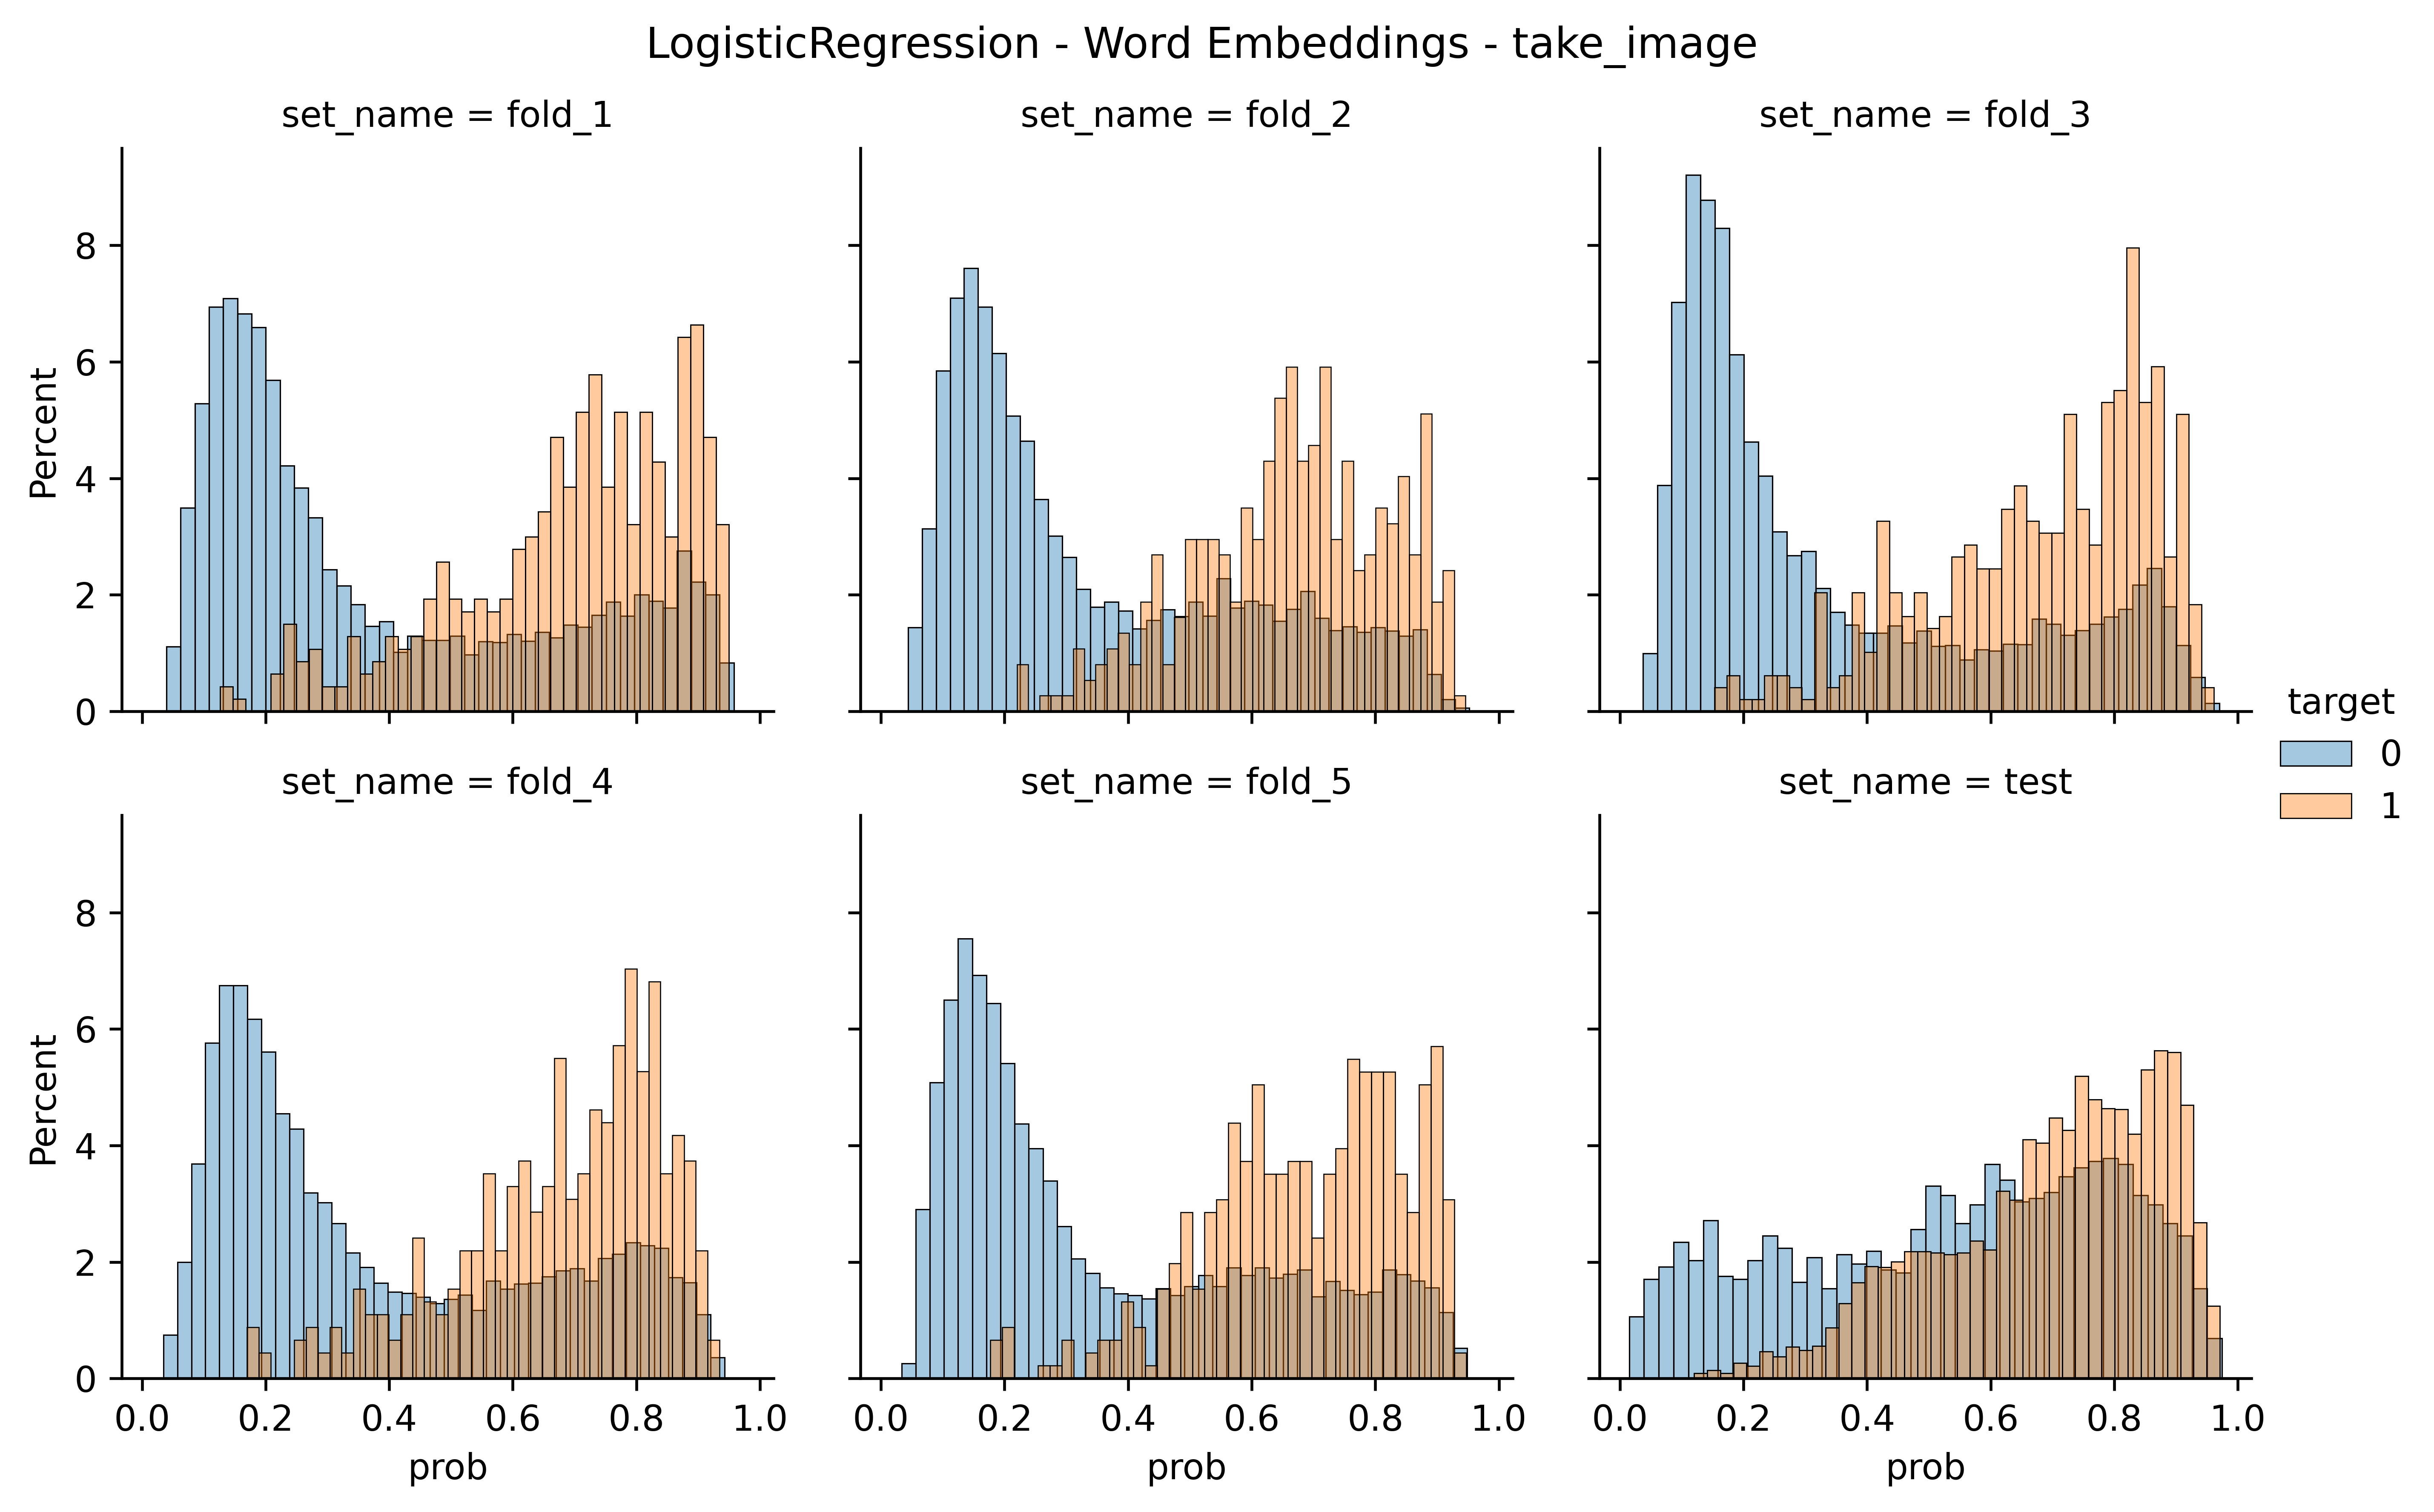
\includegraphics[width=\linewidth]{figures/results/word_embeddings/lgr/take_image/lgr__distplot.png}
        \caption{Distribución de predicciones en validación cruzada y el conjunto de test.}
        \label{fig:takeimage-bestmodel-distplot}
    \end{subfigure}
    \hfill
    \begin{subfigure}[b]{\textwidth}
    \minipage{0.32\textwidth}
      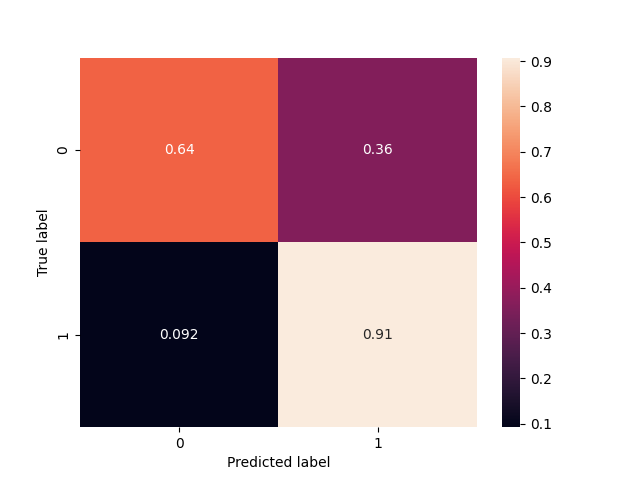
\includegraphics[width=\linewidth]{figures/results/word_embeddings/lgr/take_image/lgr_set_1_confusion_matrix_percent.png}
    \endminipage\hfill
    \minipage{0.32\textwidth}
      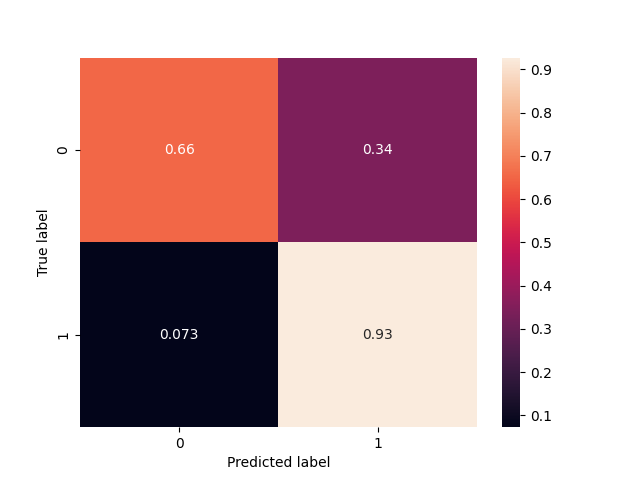
\includegraphics[width=\linewidth]{figures/results/word_embeddings/lgr/take_image/lgr_set_2_confusion_matrix_percent.png}
    \endminipage\hfill \minipage{0.32\textwidth}%
      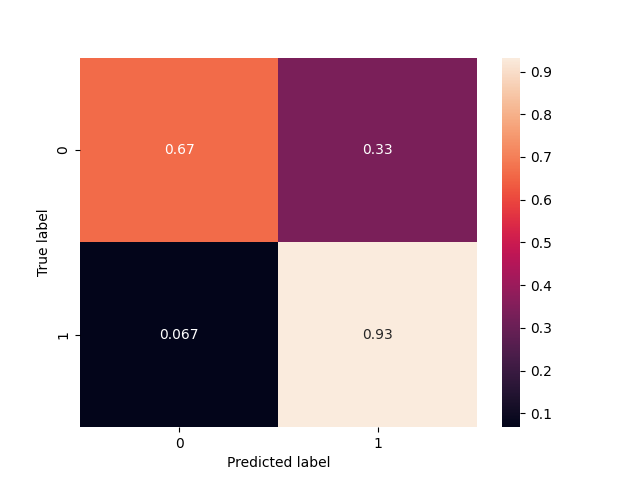
\includegraphics[width=\linewidth]{figures/results/word_embeddings/lgr/take_image/lgr_set_3_confusion_matrix_percent.png}
    \endminipage
    
    \medskip
    
    \minipage{0.32\textwidth}
      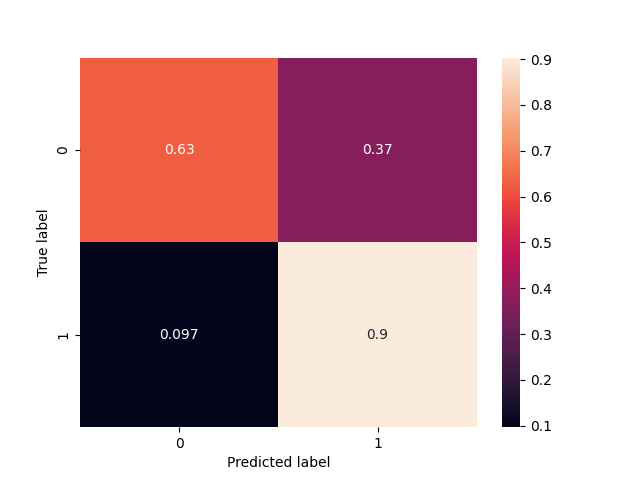
\includegraphics[width=\linewidth]{figures/results/word_embeddings/lgr/take_image/lgr_set_4_confusion_matrix_percent.png}
    \endminipage\hfill
    \minipage{0.32\textwidth}
      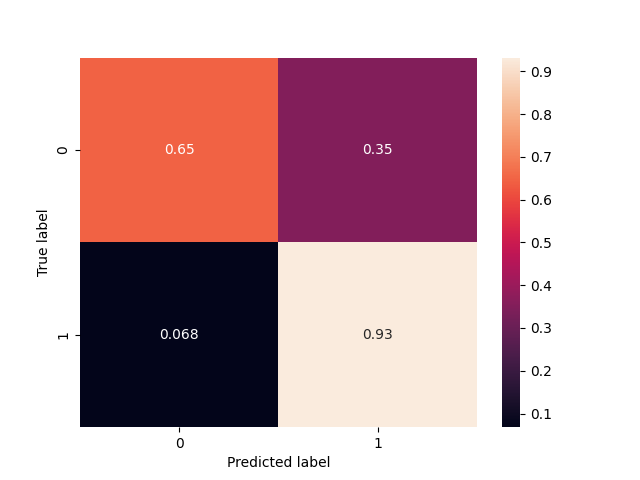
\includegraphics[width=\linewidth]{figures/results/word_embeddings/lgr/take_image/lgr_set_5_confusion_matrix_percent.png}
    \endminipage\hfill \minipage{0.32\textwidth}%
      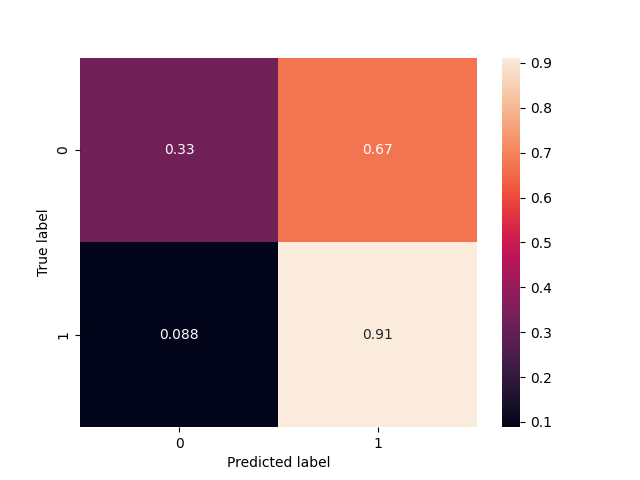
\includegraphics[width=\linewidth]{figures/results/word_embeddings/lgr/take_image/lgr_set_6_confusion_matrix_percent.png}
    \endminipage
    \caption{Matrices de confusión en validación cruzada y el conjunto de test}
    \label{fig:takeimage-bestmodel-cm}
    \end{subfigure}
    \caption{Resultados del modelo de regresión logística con codificación por word embeddings y esquema de acción take\_image.}
    \label{fig:takeimage-bestmodel}
\end{figure}


La figura muestra dos histogramas independientes, el de la clase positiva, y el
de la clase negativa. Cada punto en el gráfico representa la probabilidad de una
acción dado su plan relajado (completo). Para ambos histogramas se genera una
cantidad $N$ de bins equidistantes en el rango [0, 1]. Luego, para cada bin $b$,
se muestra la cantidad de acciones que recibieron una probabilidad contenida en
$b$ divido el tamaño de la clase a la que pertenecen.

Para el histograma de la clase positiva, observamos que las acciones relevantes
(good operators) se agrupan en los bins con probabilidades entre $r=[0,6; 1]$.
Cada bin contiene entre el 2\% al 7\% de las acciones. Si sumamos los
porcentajes de cada uno de los bins en $r$, tendremos que más de la mitad de las
acciones se encuentran en $r$.

Por otro lado, el histograma de la clase negativa, muestra que más de la mitad
de las acciones no relevantes (bad operators) se agrupan en los bins con
probabilidades entre $[0;0.4]$.

Desde el punto de vista de grounding heurístico este es el comportamiento que
buscamos. El algoritmo almacenará en una cola de prioridades acciones tanto
relevantes como no relevantes con una probabilidad asociada, dándole prioridad a
las que tienen una mayor probabilidad. Si el modelo asigna a las acciones
relevantes una alta probabilidad entonces el proceso de grounding heurístico les
dará prioridad para su instanciación.

Notar que el objetivo de utilizar validación cruzada es variar el conjunto de
entrenamiento con el fin de determinar si el modelo de LGR es robusto ante
cambios, lo cual podemos decir que indudablemente fue este el caso en las 5
particiones.

Si observamos la matriz de confusión del modelo por cada partición dada por la
figura \ref{fig:takeimage-bestmodel-cm}, podemos ver que en cada uno, más del
90\% de las acciones positivas se predicen como positivas, y más del 63\% de las
negativas se predicen como negativas. La función de decisión se obtiene a partir
del cálculo de $H_{1.5}$. Es decir, se computa $H_{1.5}$ para distintas
funciones de decisión con umbral en el intervalo [0, 1] y utilizamos aquel que
maximice $H_{1.5}$. 

\subsubsection{Performance en test}

Los resultados anteriores fueron sobre 5 particiones del conjunto de
entrenamiento donde una parte efectivamente se utilizaba para entrenar el modelo
y otra para su evaluación. Sin embargo, lo que buscamos es que esto mismo se
logre generalizar a problemas no instanciables. Por lo tanto, la evaluación
final la realizamos sobre el conjunto de test.

\begin{figure}
    \centering
    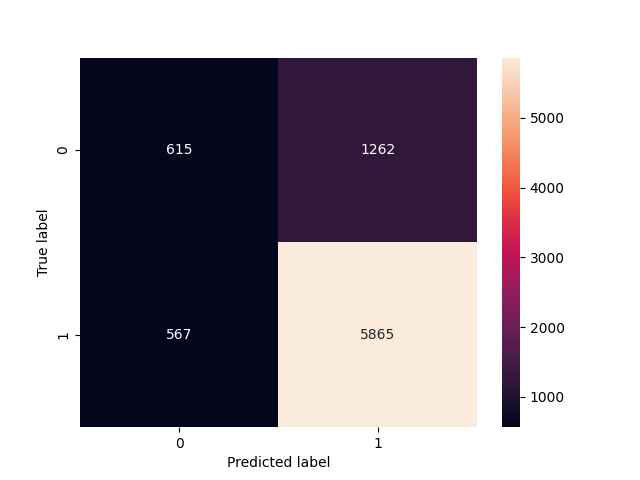
\includegraphics[scale=0.7]{figures/results/word_embeddings/lgr/take_image/lgr_set_6_confusion_matrix_raw.png}
    \caption{Matriz de confusión sin porcentajes del modelo de regresión logística con codificación por word embeddings y esquema de acción take\_image.}
    \label{fig:takeimage-bestmodel-cm-raw}
\end{figure}

La figura \ref{x} muestra nuevamente muestra un histograma de la probabilidad de
una acción dado su plan relajado. El caso de las acciones relevantes se sigue
manteniendo el comportamiento que vimos en validación cruzada lo cual es un buen
indicio ya que estarán en las primeras posiciones en la cola de prioridades en
grounding heurístico. Sin embargo, si observamos el histograma de acciones no
relevantes, se tiene que ahora a una gran parte de ellas se le asigna una alta
probabilidad. Estas acciones también serían ubicadas al comienzo de la cola de
prioridades y por lo tanto instanciadas. Si observamos la matriz de confusión en
\ref{x'}, la proporción de acciones relevantes se mantiene en un 91\%, mientras
que esta vez un 67\% de las no relevantes se filtran como positivas, cabe
recalcar que esta vez, el umbral de decisión en test es el promedio de los
umbrales obtenidos en validación cruzada. El objetivo era aprender un umbral que
sea lo más óptimo para predecir nuevos ejemplos, utilizando únicamente
información de los datos de entrenamiento. Podríamos haber utilizado un umbral
de decisión a partir de las etiquetas de test, no obstante tal predicción
representaría la performance máxima o ideal que podríamos obtener en test, y no
la que realmente estamos obteniendo con información del conjunto de
entrenamiento.

Por último, si observamos la matriz de confusión de la figura
\ref{fig:takeimage-bestmodel-cm-raw} del modelo LGR, pero esta vez sin
normalizar por porcentajes. Se puede ver que LGR tiende a predecir ligeramente
sobre la clase positiva, pero además es la mayoritaria en test para este
esquema. Esto sucede debido a como se generan los bad operators en los problemas
de test. Recordemos que estos no pueden obtenerse por Fast Downward por lo que
se generó una muestra aleatoria usando grounding cartesiano pero respetando los
tipos de las interfaces. Como solo se pudieron generar una cantidad de 5000 bad
operators por problema, y los planes en los problemas de test son de mayor
tamaño que los de entrenamiento, surgió este desbalance hacia la clase positiva.
No obstante, en una situación real, la cantidad de bad operators sería
nuevamente superior a la de good operators. Otro aspecto importante sobre la
generación de los bad operators es que podrían no ser alcanzables relajadamente,
y por lo tanto tener una distribución distinta a la que tenemos en el conjunto
de entrenamiento siendo una de las posibles causas del desempeño de LGR para la
clase negativa. Es decir, LGR fue entrenado para predecir, sobre acciones
alcanzables relajadamente, pero lo estamos evaluando sobre bad operators que no
lo son.

Por último, notar que precision y recall sobre la clase positiva es de 0.823, y
0.912, respectivamente. Si calculamos la métrica $F_{1.5}$ priorizando recall,
obtendriamos una performance de 0.8826 para LGR. Sin embargo, no es un buen
indicio de la correctitud del modelo en la clase negativa, como podemos ver en
el cuadro \ref{results:lgr-wb-calibrate}. En contraparte, si en lugar de
considerar $F_{1.5}$ utilizamos $H_{1.5}$ la performance es de 0.589 lo cual
al penalizar la baja en la taza de verdaderos negativos.

\begin{table}[h!]
\centering
\scalebox{0.9}{
 \begin{tabular}{|c || c | c | c | c | c | c |} 
 \hline
  Clase & Precisión & Recall & $H_{1.5}$ & $F_{1.5}$ & Umbral de decisión \\
 \hline
 Relevante & 0.823 & 0.912 & 0.589 & 0.8826 & 0.416 \\
 No relevante & 0.52 & 0.33 & 0.4081 & 0.3717 & 0.416 \\
 \hline
 \end{tabular}}
 \caption{Resultados por esquema de acción del mejor modelo con codificación por word embeddings.}
 \label{results:lgr-wb-calibrate}
\end{table}

\begin{figure}
    \centering
    \begin{subfigure}[b]{0.83\textwidth}
    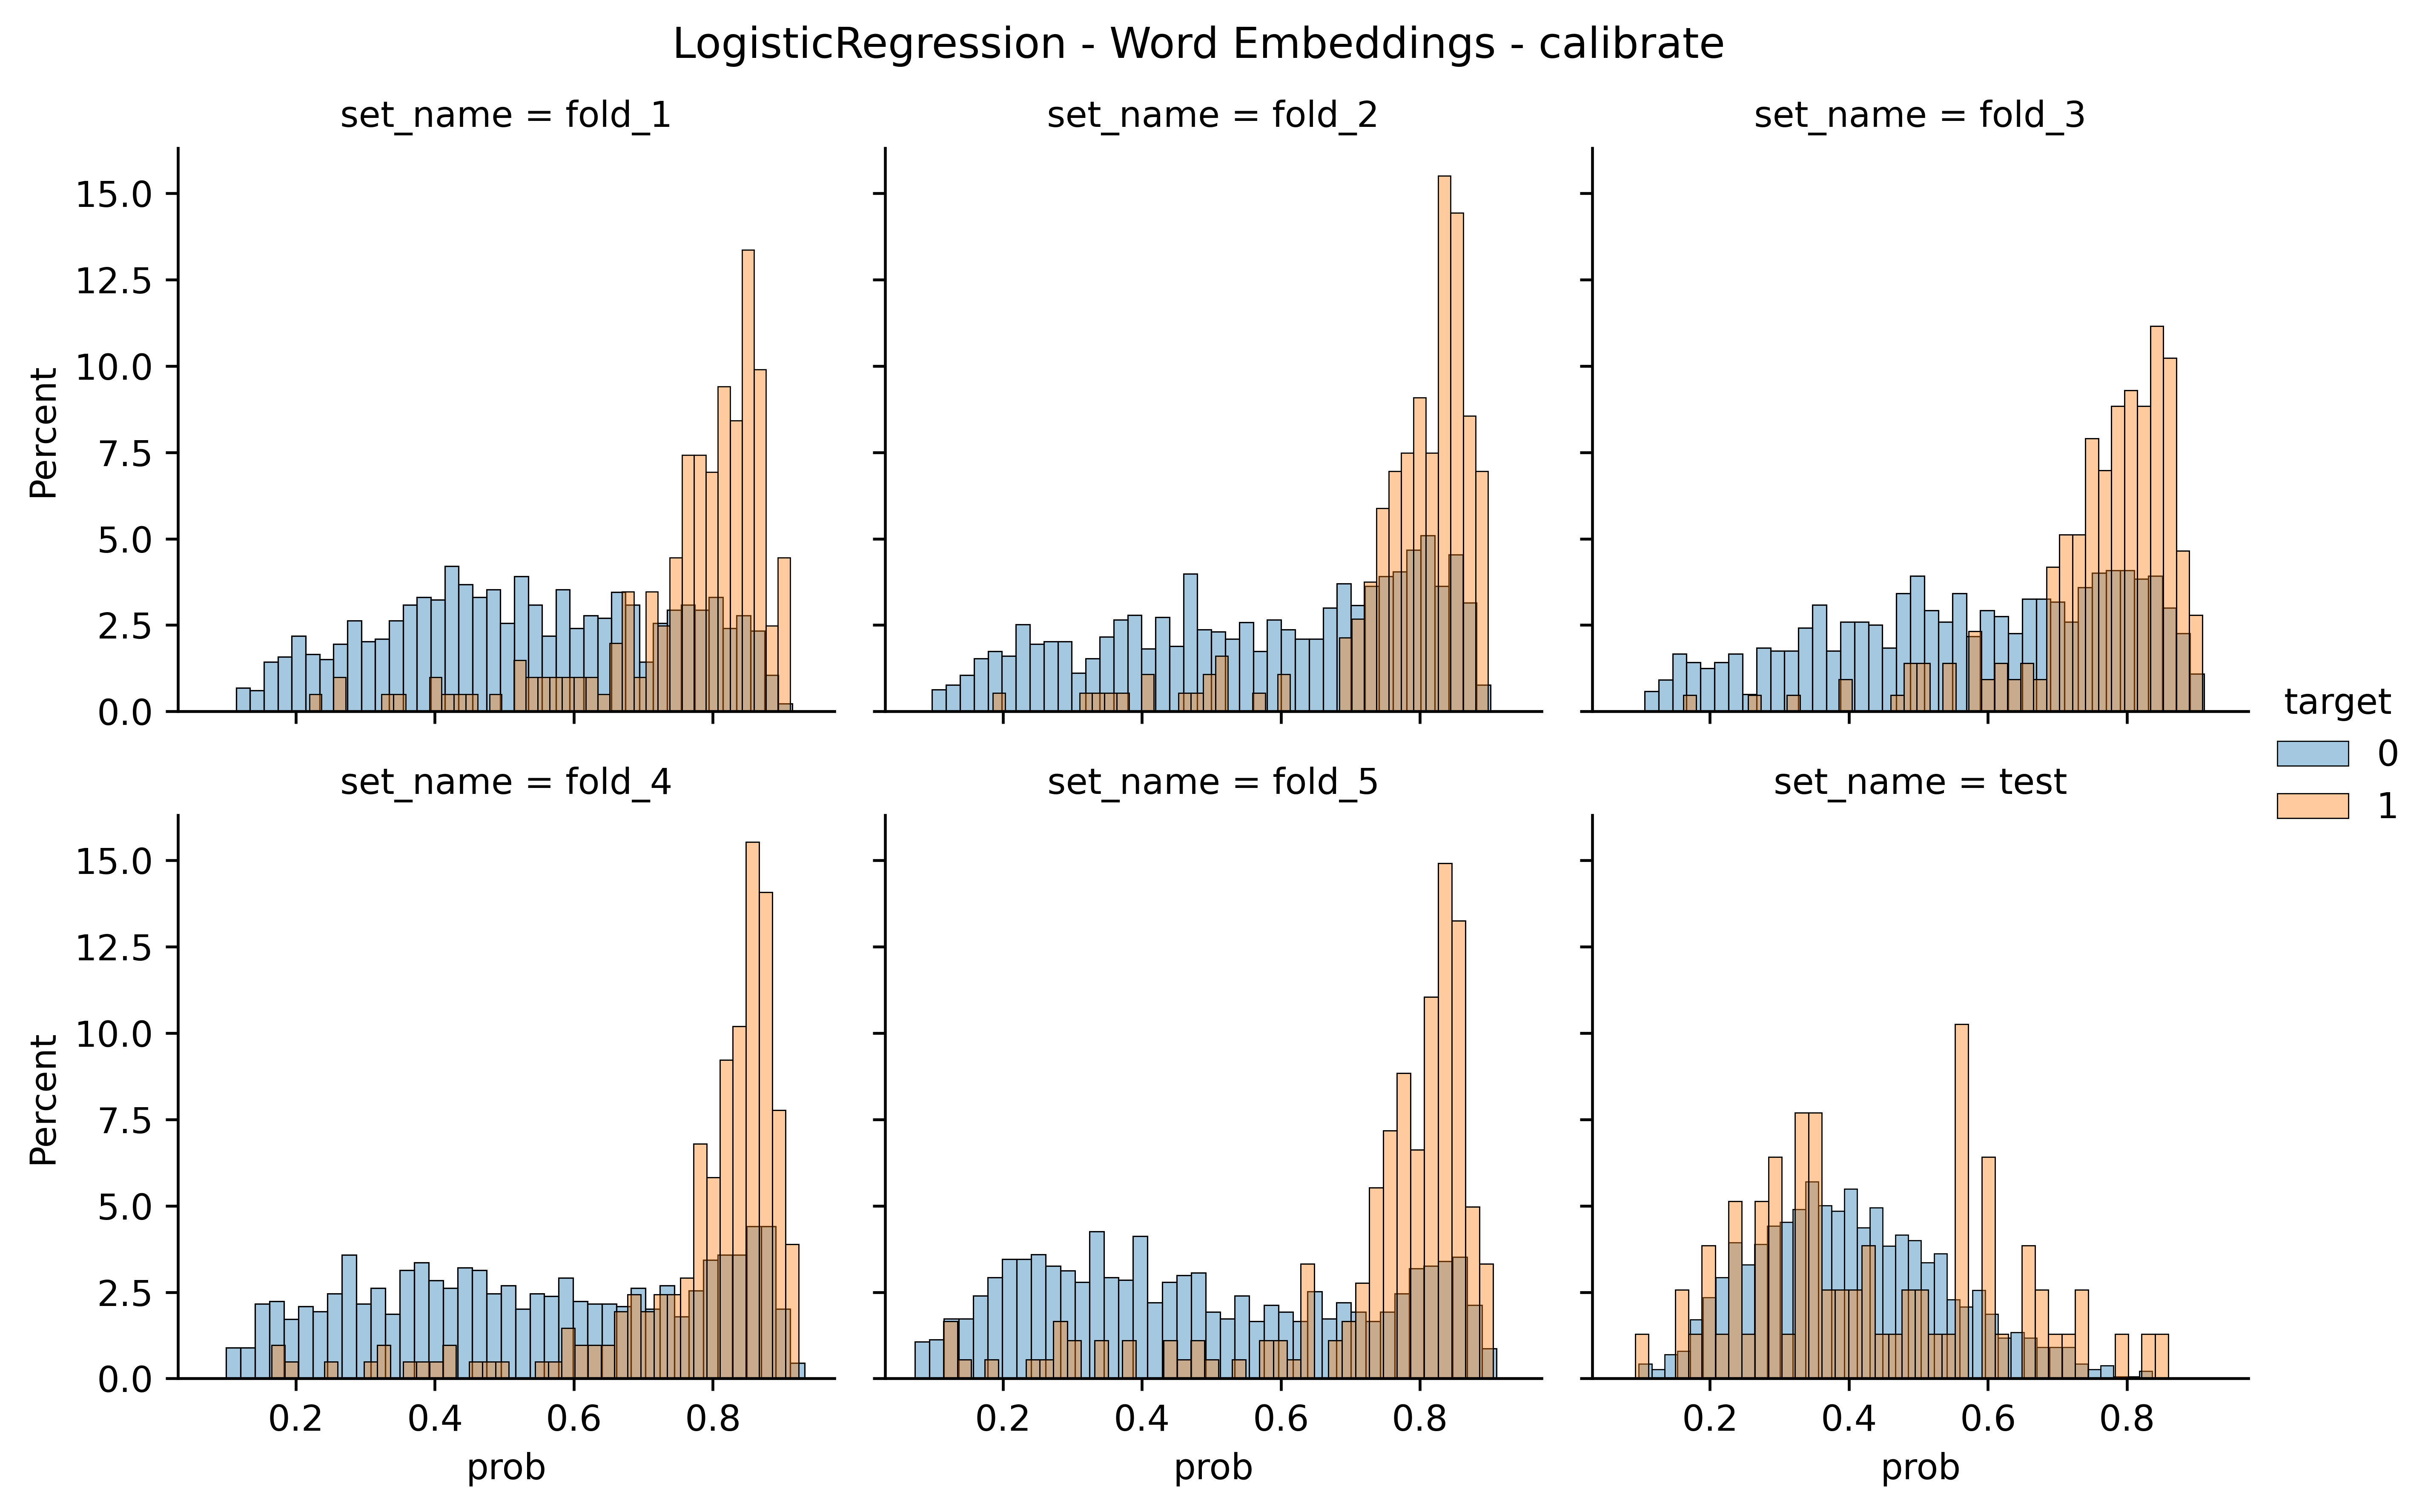
\includegraphics[width=\linewidth]{figures/results/word_embeddings/lgr/calibrate/calibrate__distplot.png}
    \end{subfigure}
    \hfill
    \centering
    \begin{subfigure}[b]{0.83\textwidth}
        \centering
        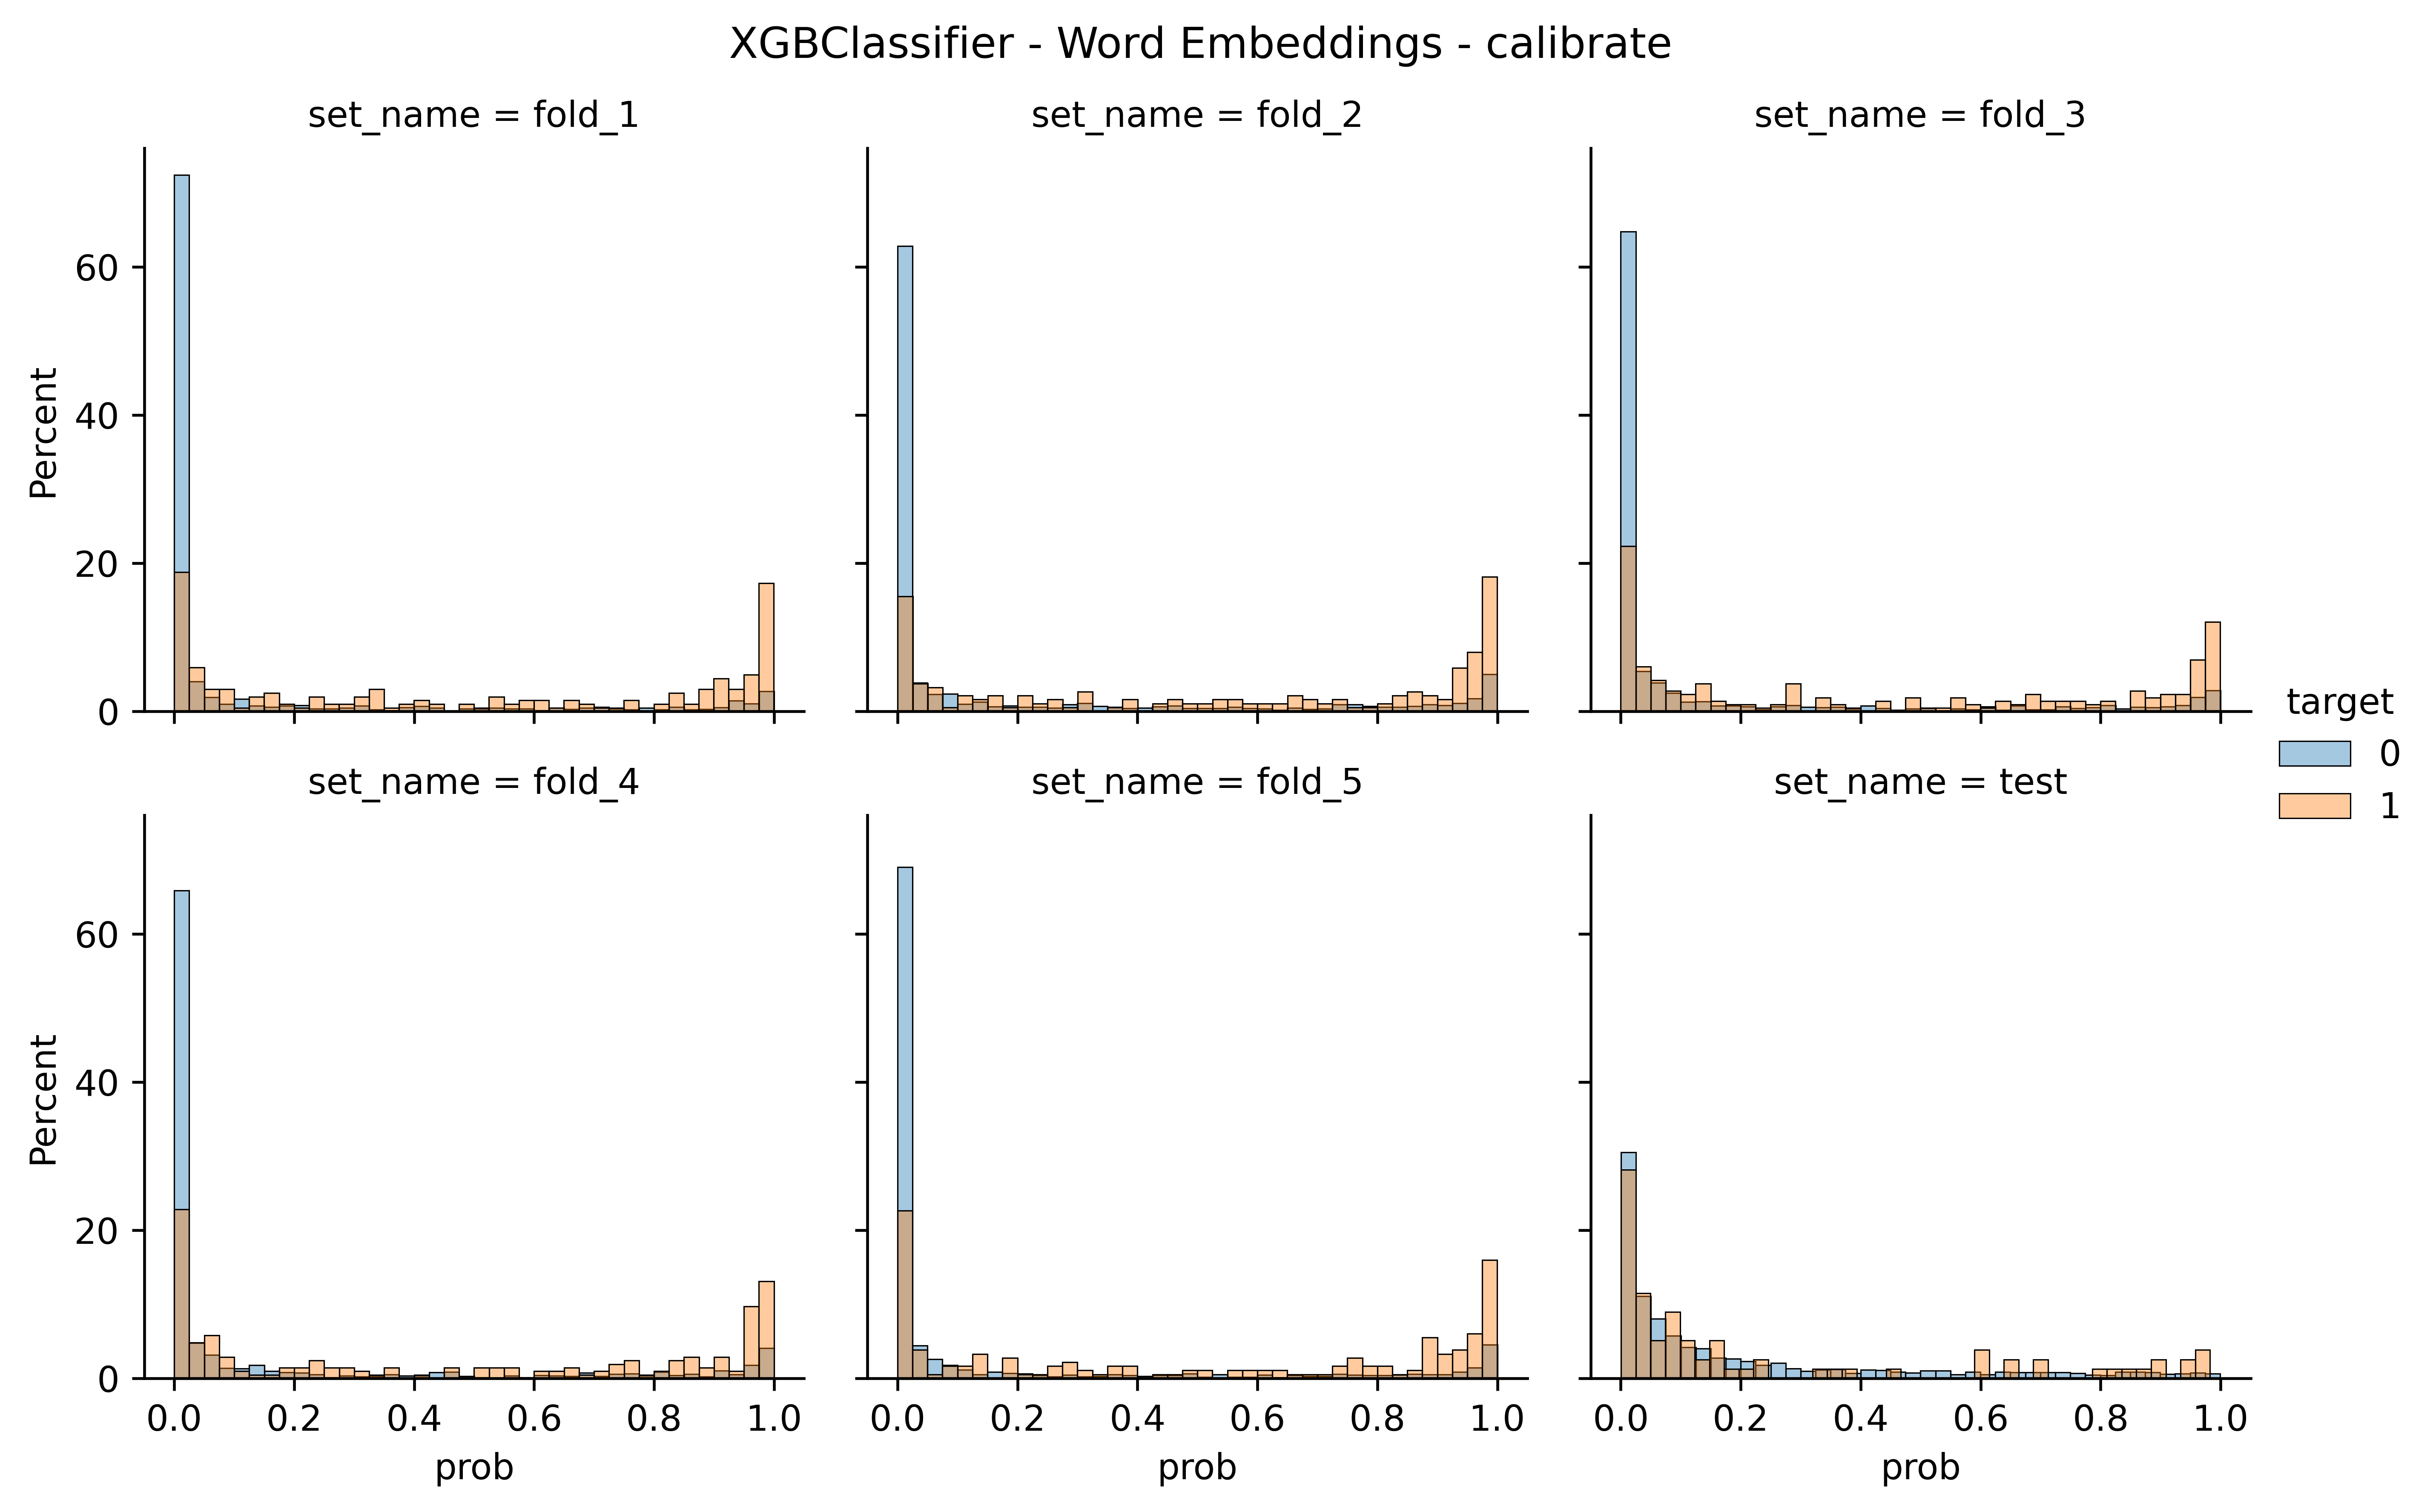
\includegraphics[width=\linewidth]{figures/results/word_embeddings/xgboost/calibrate/calibrate__distplot.png}
    \end{subfigure}
    \hfill
    \centering
    \begin{subfigure}[b]{0.83\textwidth}
        \centering
        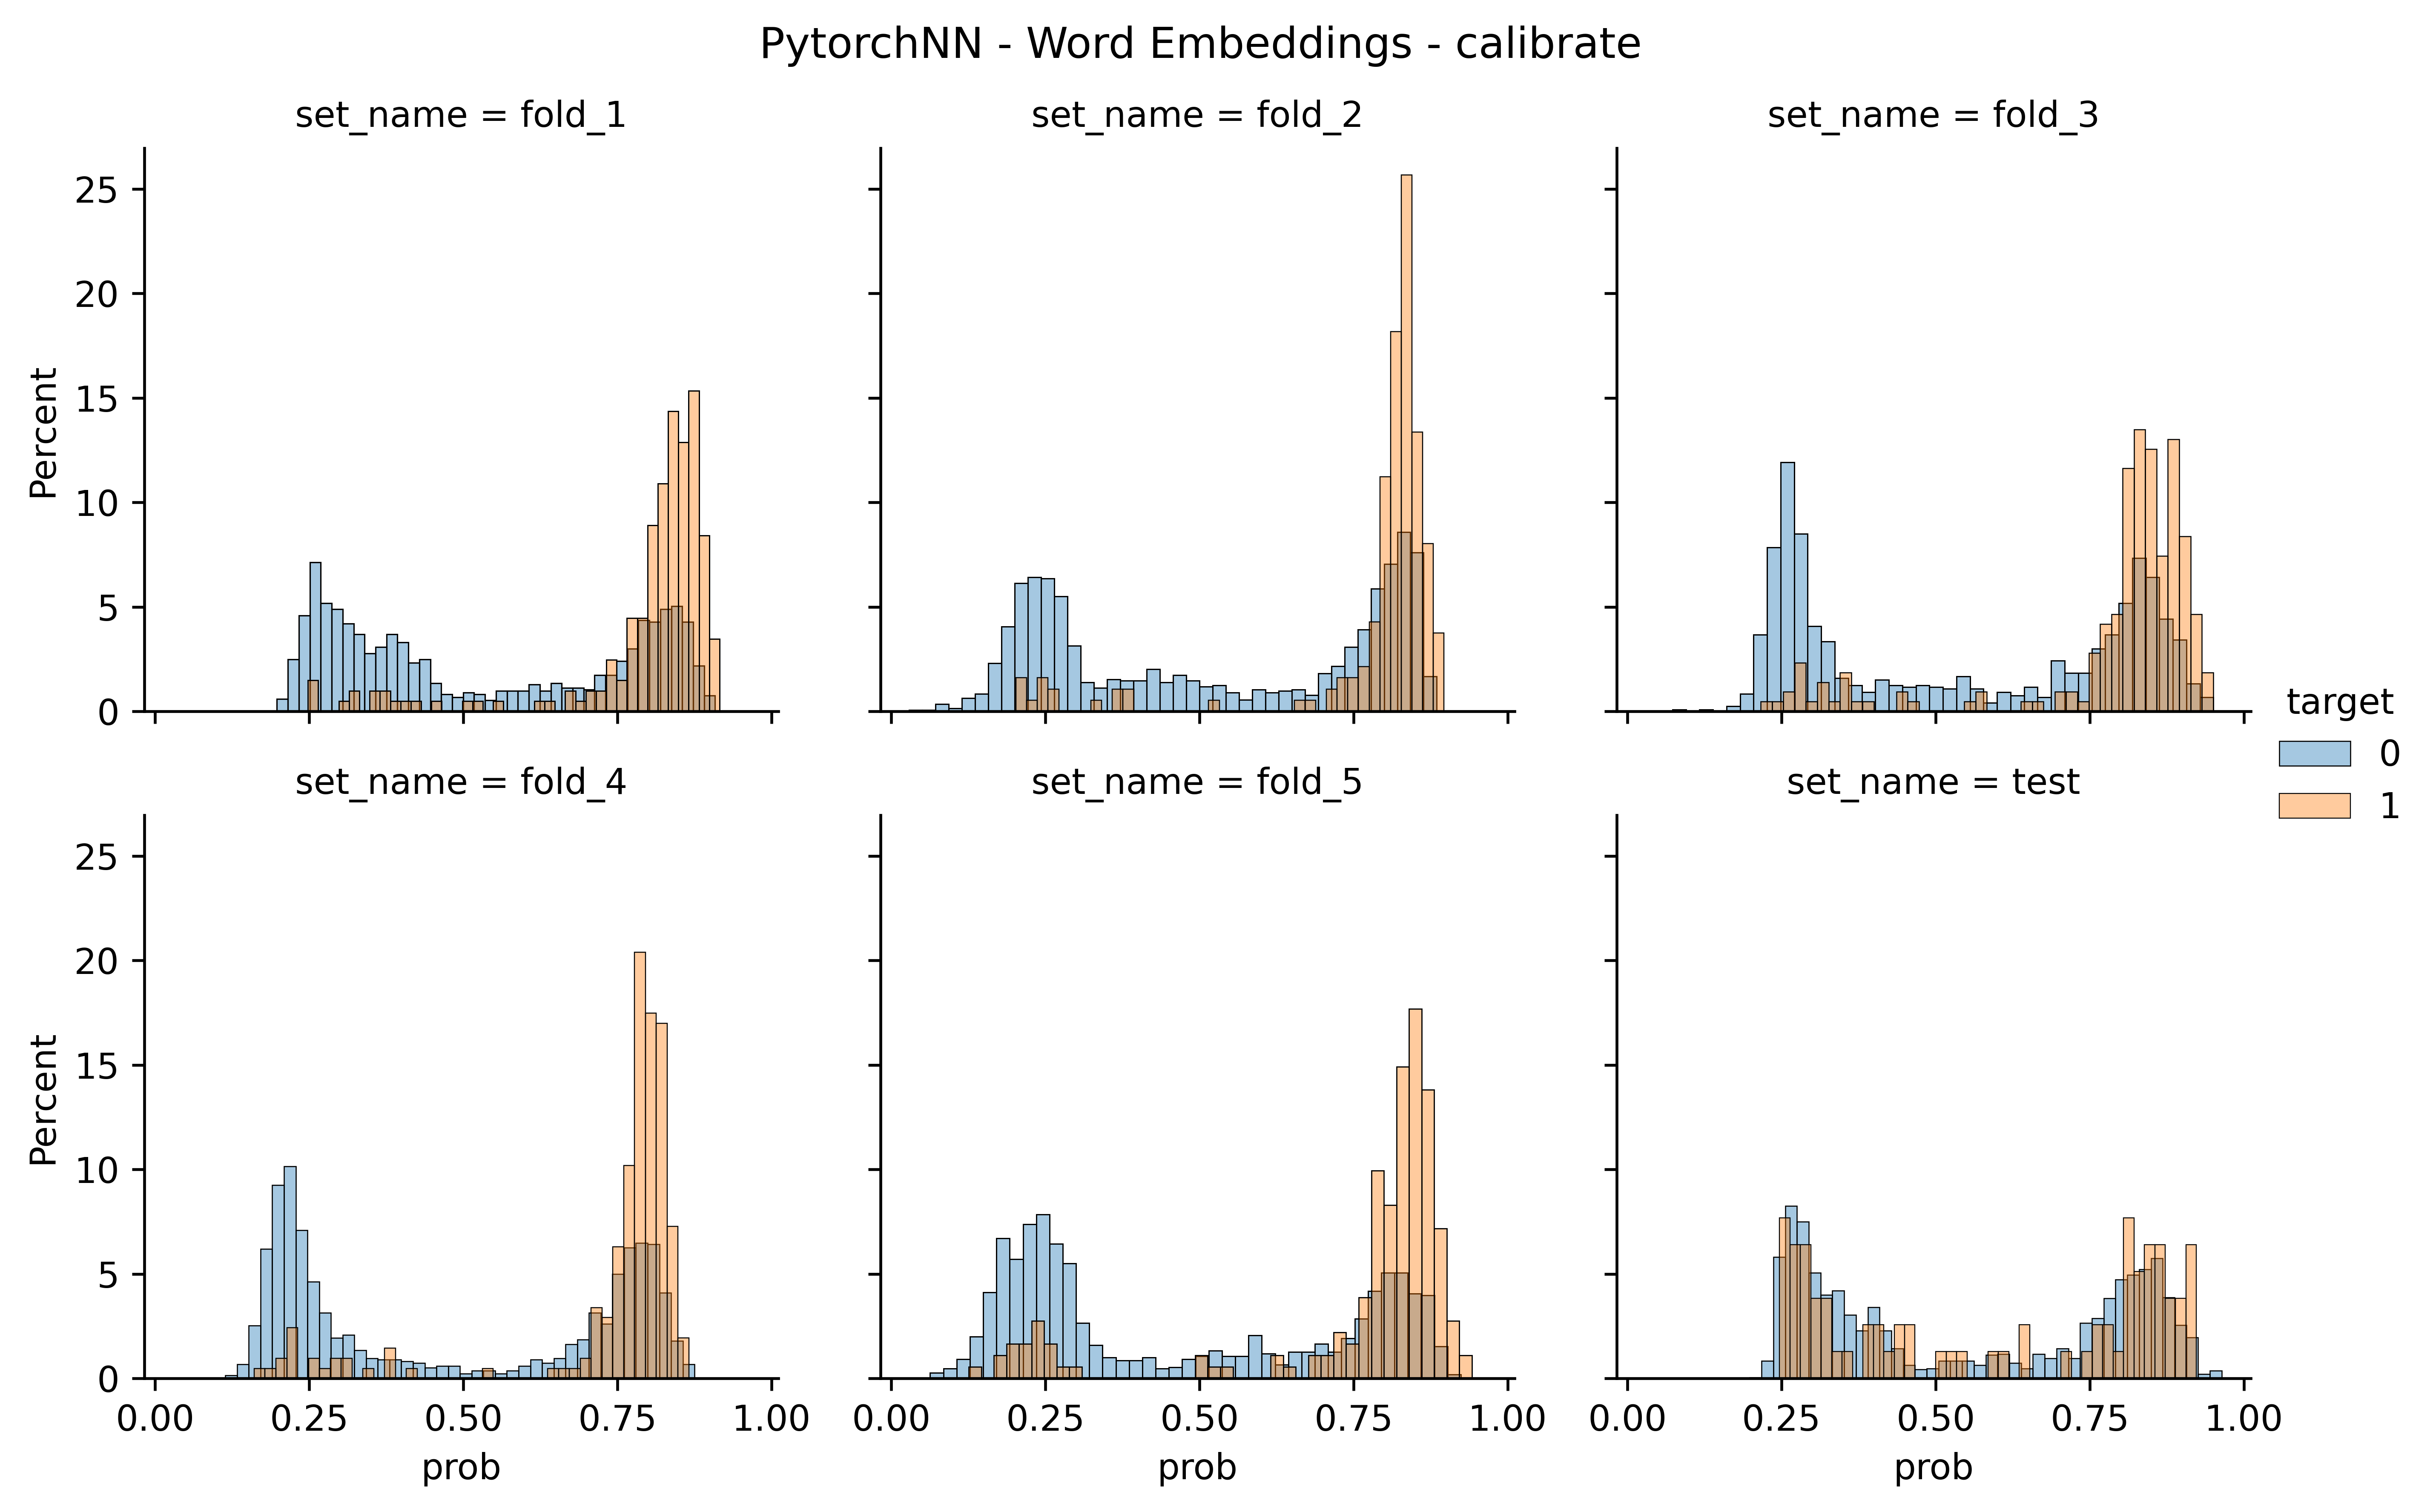
\includegraphics[width=\linewidth]{figures/results/word_embeddings/nn/calibrate/calibrate__distplot.png}
    \end{subfigure}
    \caption{Word embeddings calibrate}
\end{figure}

\begin{figure}
    \centering
    \begin{subfigure}[b]{0.83\textwidth}
    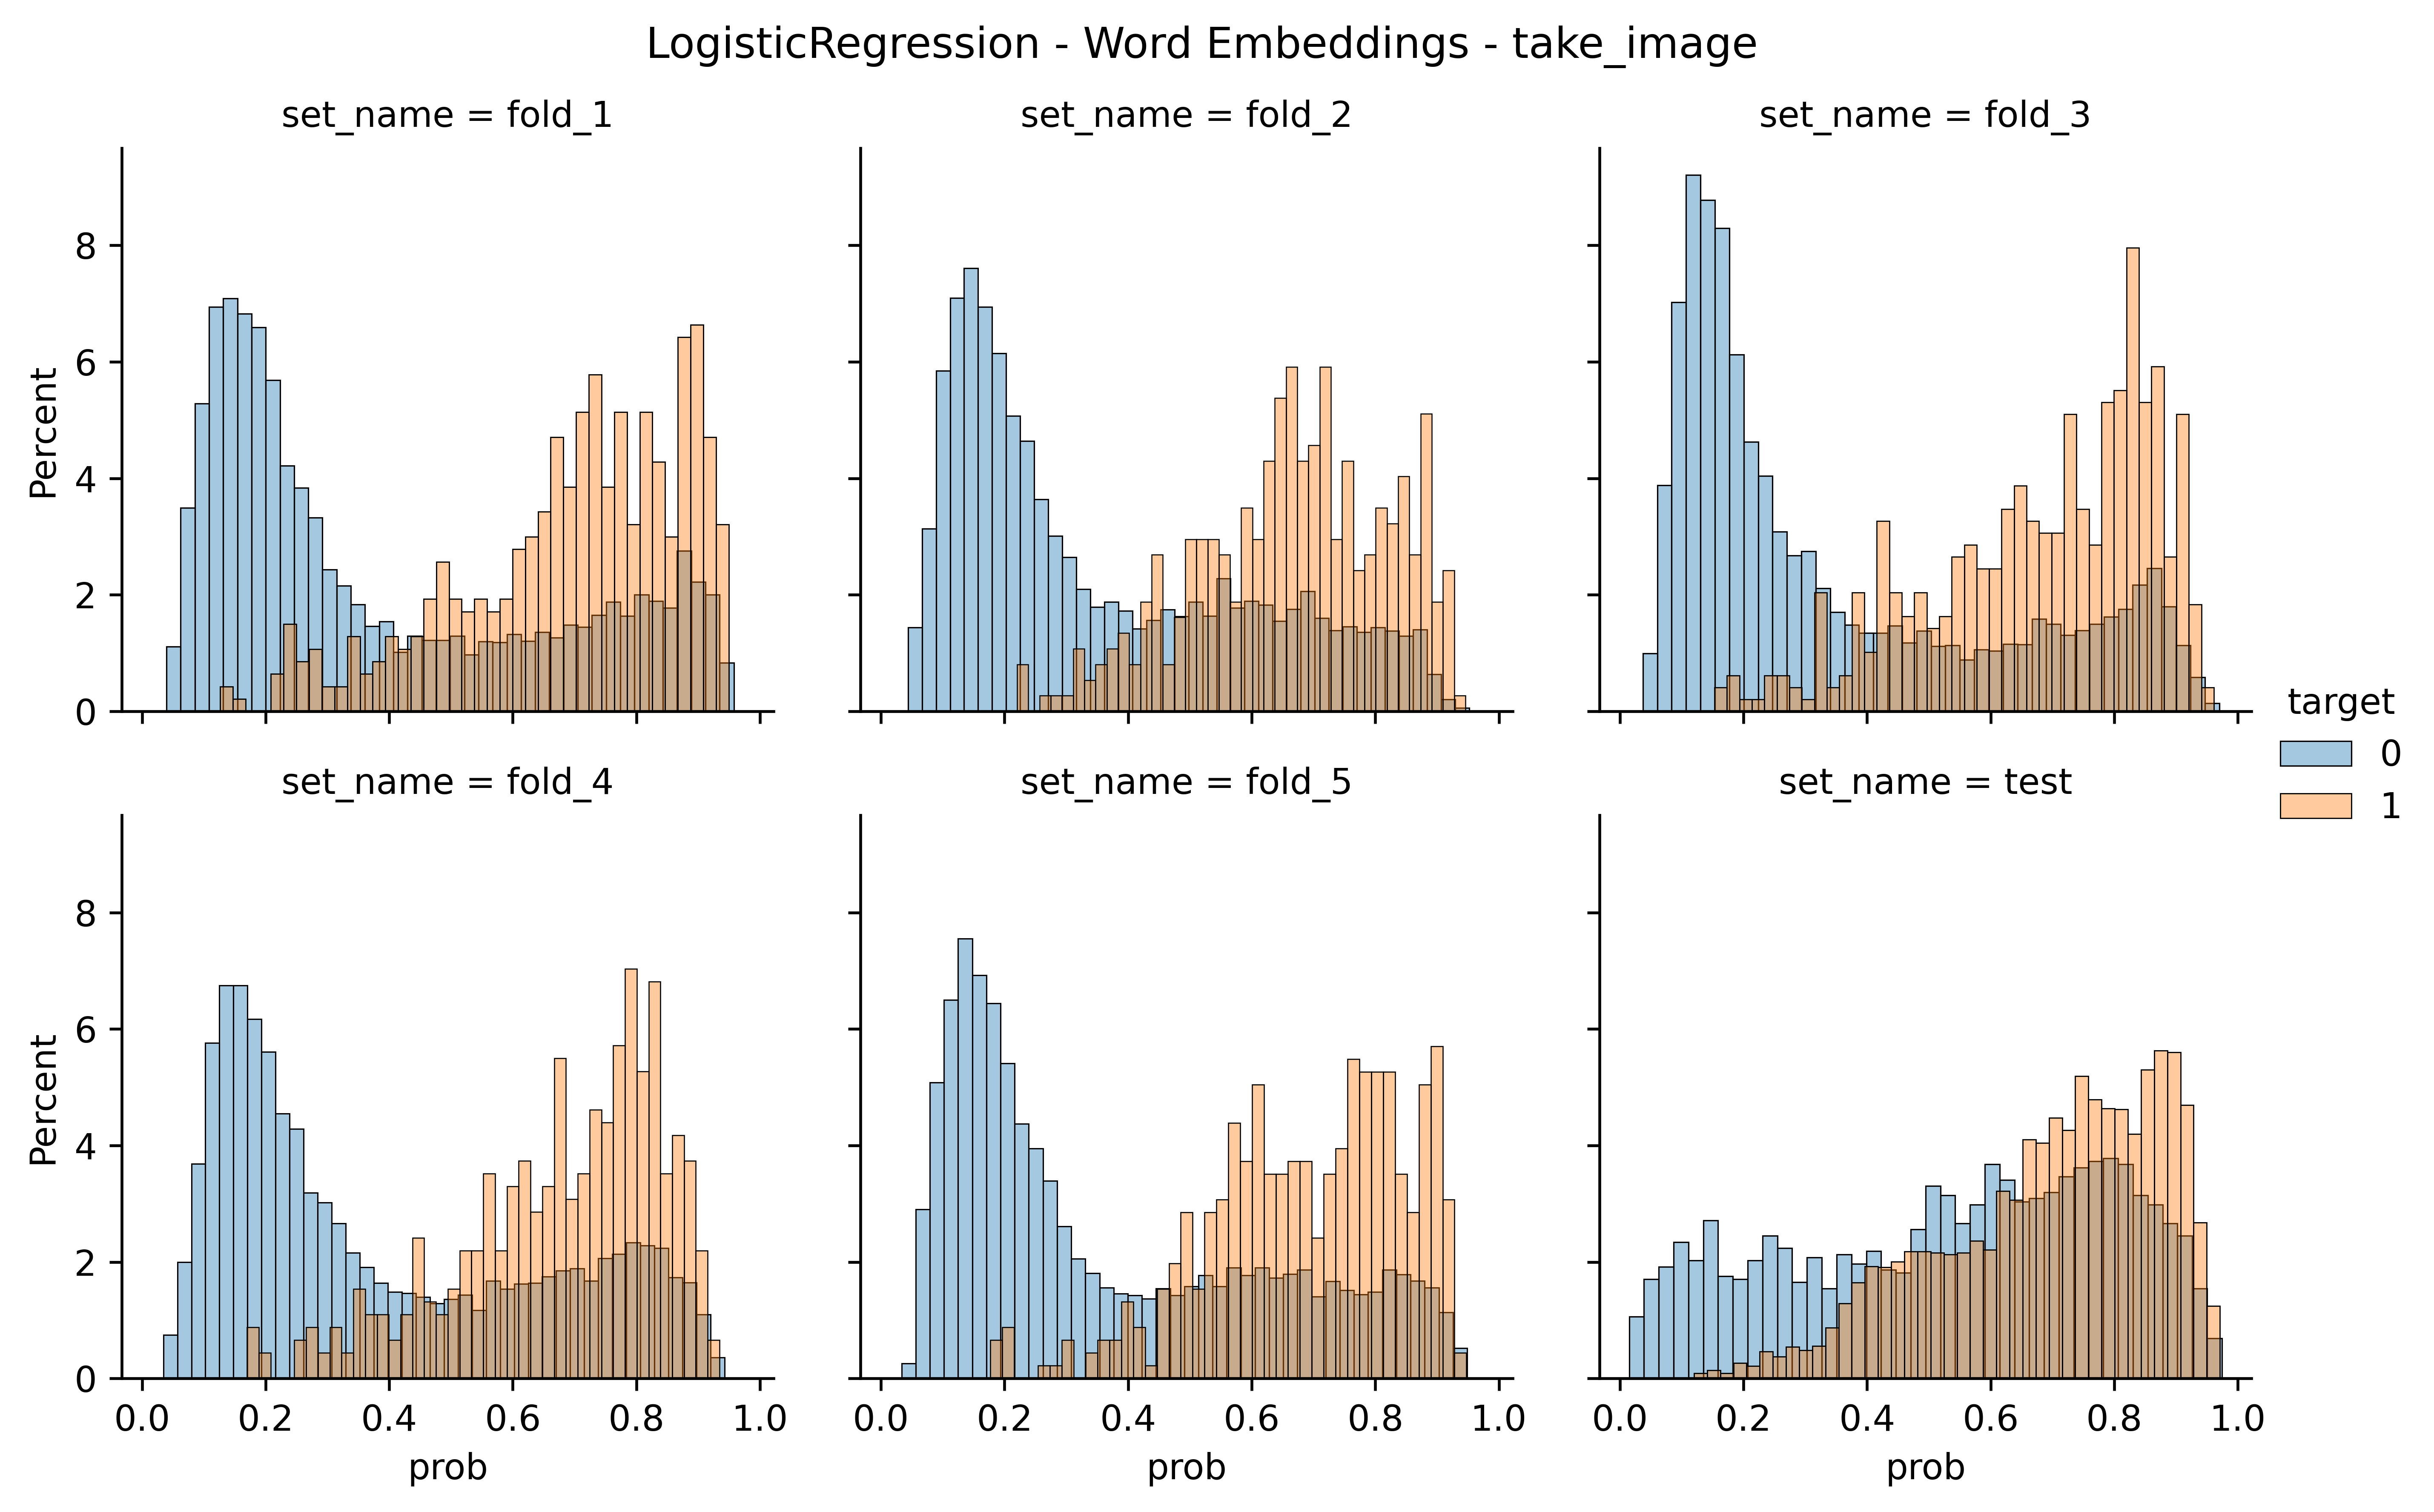
\includegraphics[width=\linewidth]{figures/results/word_embeddings/lgr/take_image/lgr__distplot.png}
    \end{subfigure}
    \hfill
    \centering
    \begin{subfigure}[b]{0.83\textwidth}
        \centering
        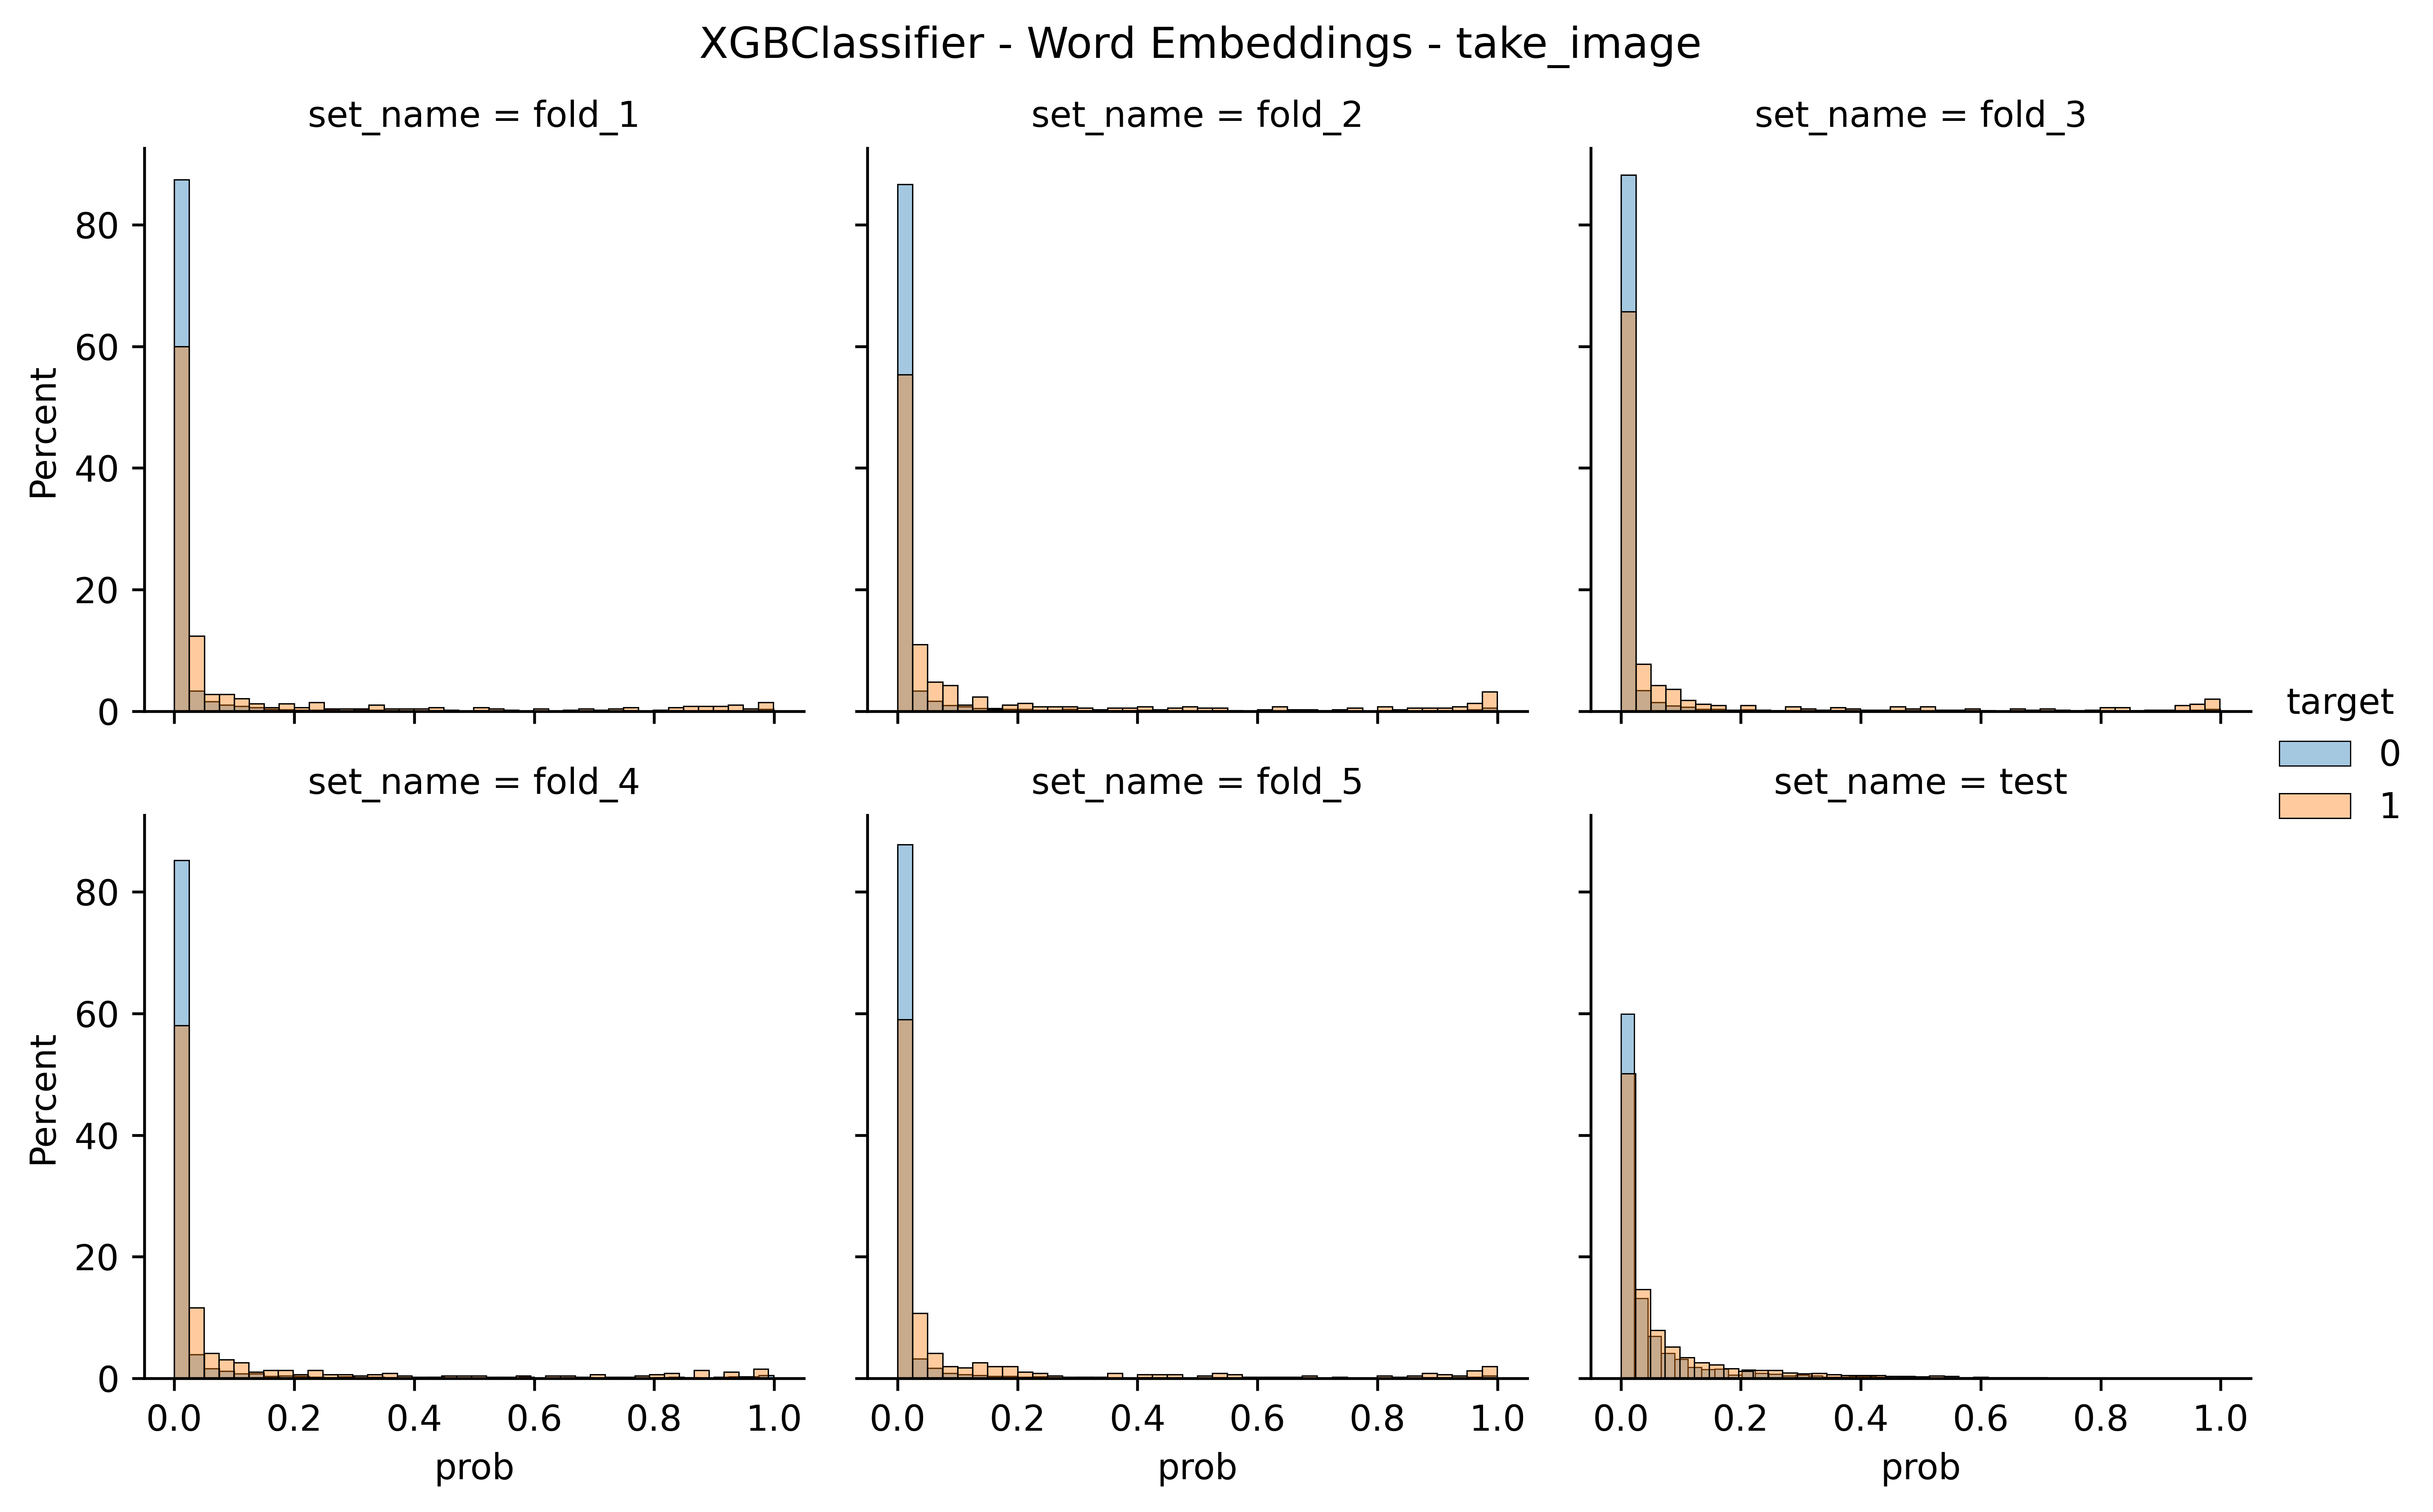
\includegraphics[width=\linewidth]{figures/results/word_embeddings/xgboost/take_image/take_image__distplot.png}
    \end{subfigure}
    \hfill
    \centering
    \begin{subfigure}[b]{0.83\textwidth}
        \centering
        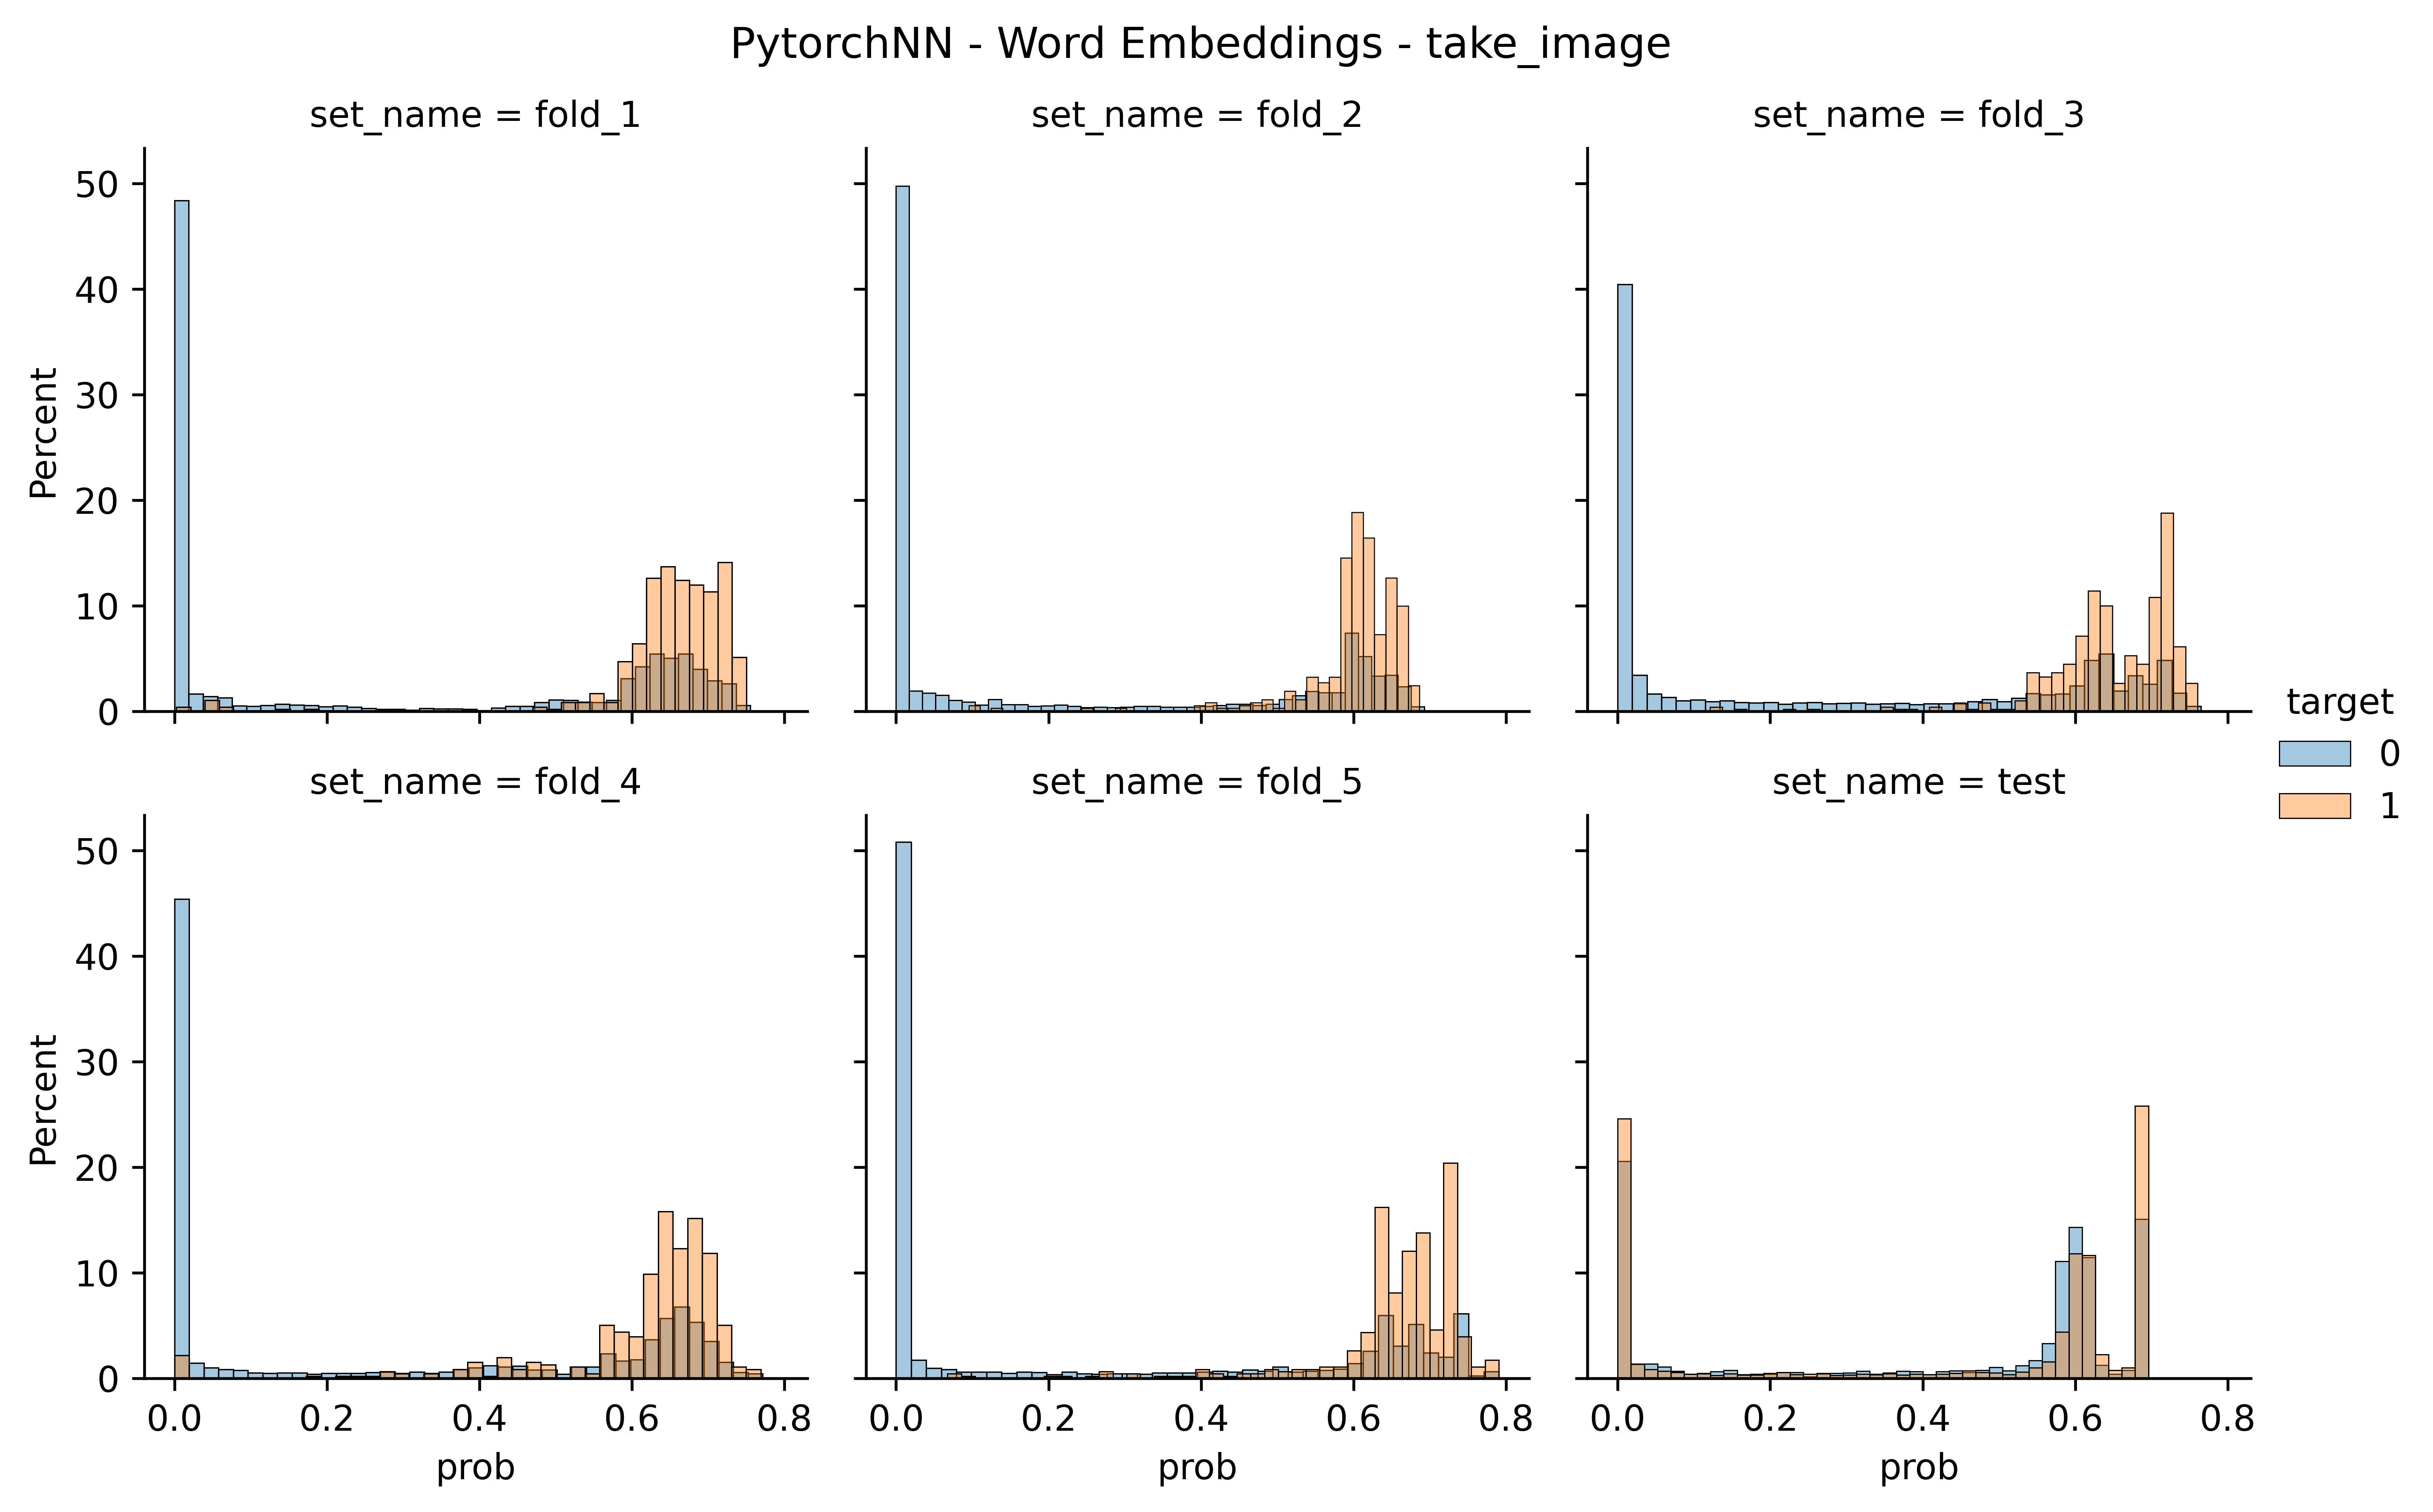
\includegraphics[width=\linewidth]{figures/results/word_embeddings/nn/take_image/take_image__distplot (1).png}
    \end{subfigure}
    \caption{Word embeddings take\_image}
\end{figure}

\begin{figure}
    \centering
    \begin{subfigure}[b]{0.83\textwidth}
    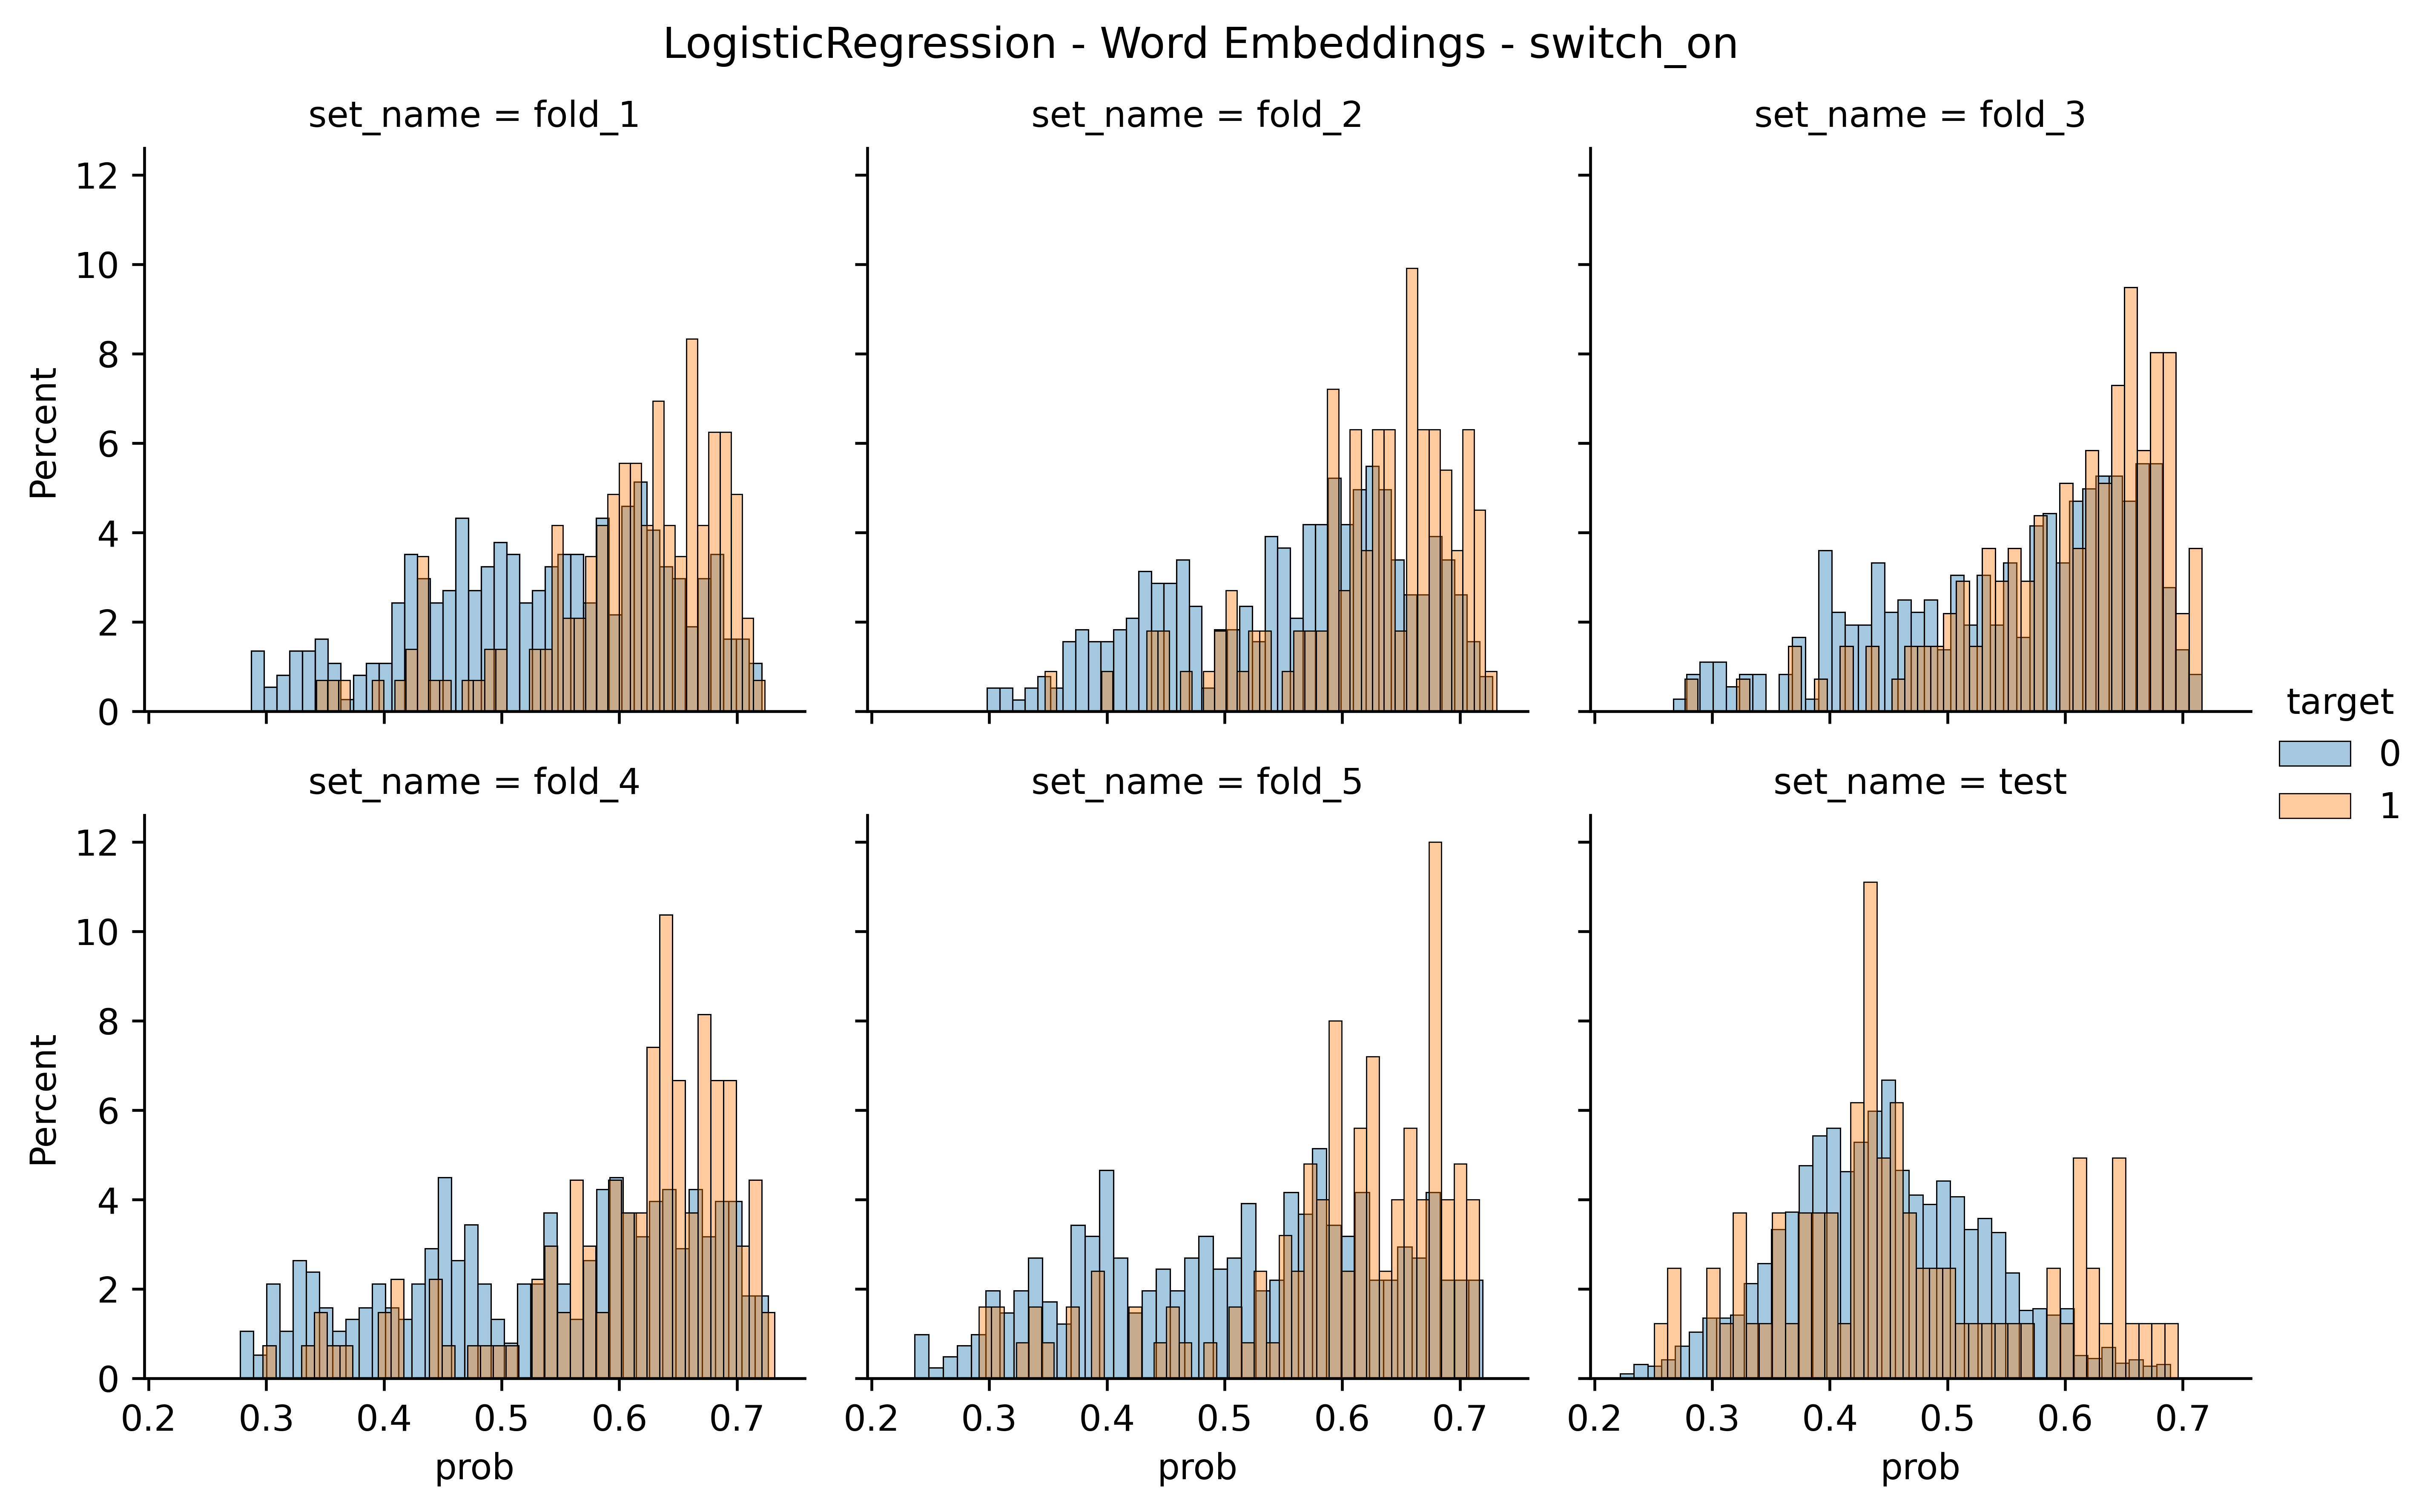
\includegraphics[width=\linewidth]{figures/results/word_embeddings/lgr/switch_on/switch_on__distplot.png}
    \end{subfigure}
    \hfill
    \centering
    \begin{subfigure}[b]{0.83\textwidth}
        \centering
        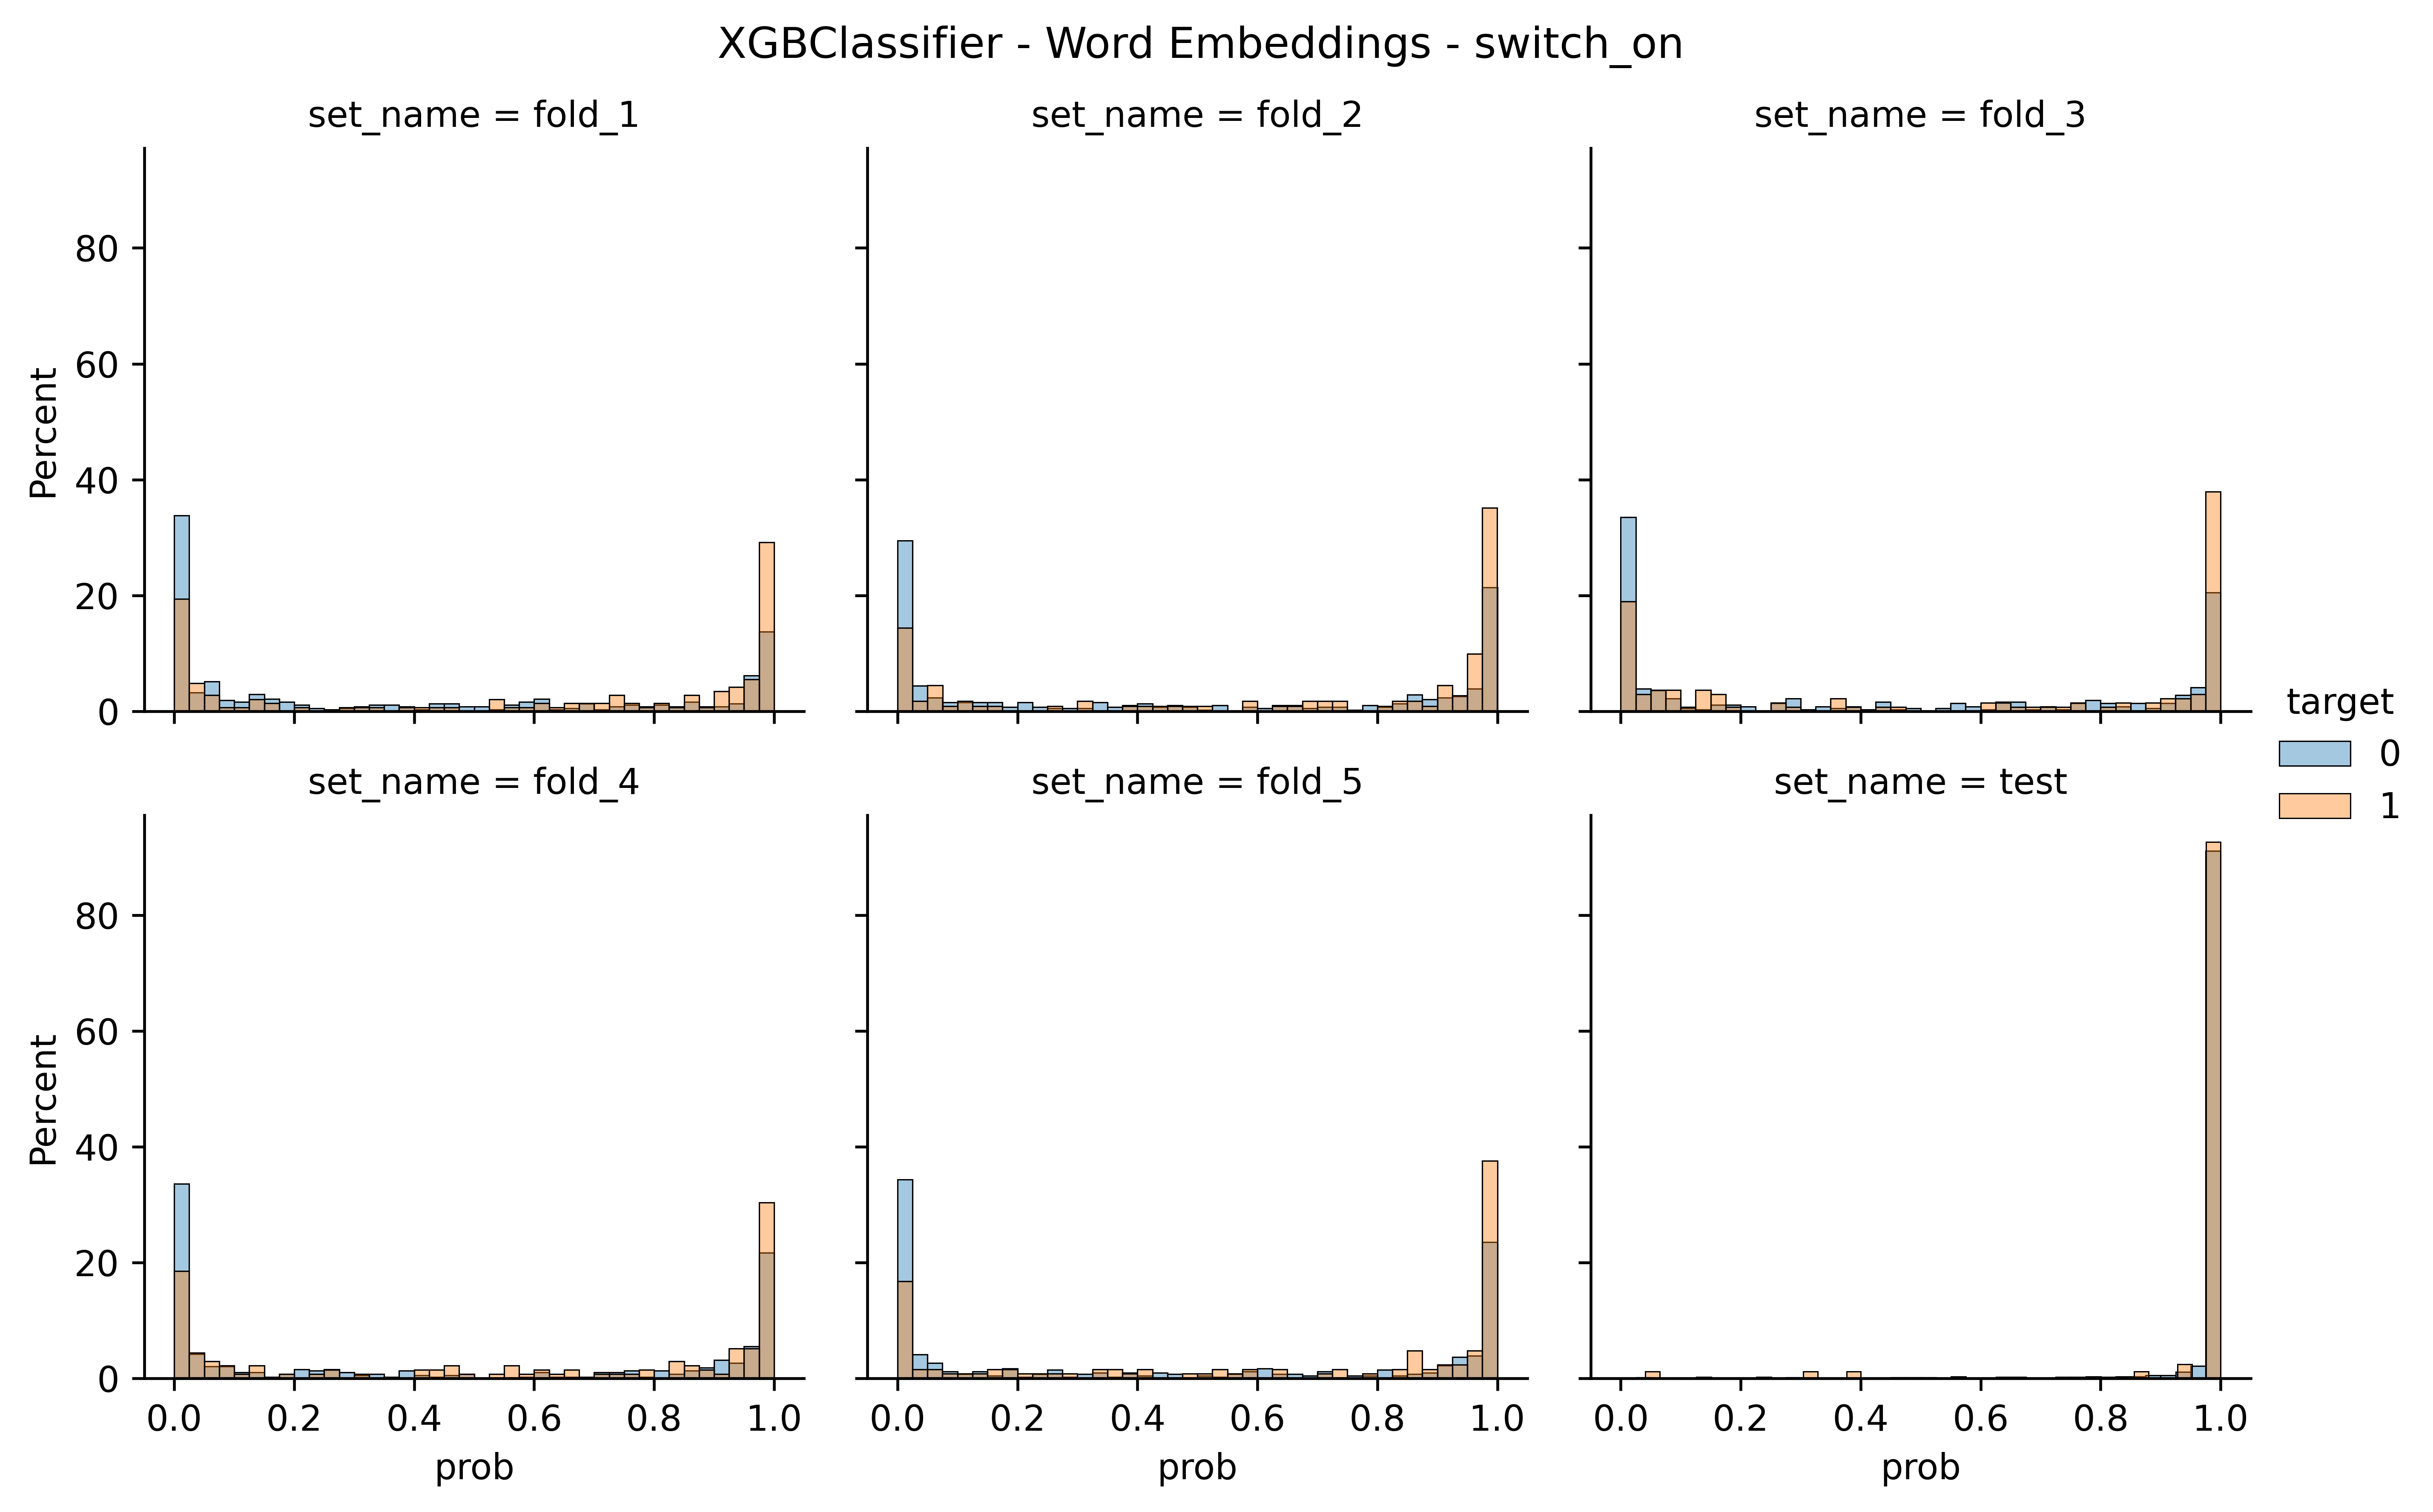
\includegraphics[width=\linewidth]{figures/results/word_embeddings/xgboost/switch_on/xgb__distplot.png}
    \end{subfigure}
    \hfill
    \centering
    \begin{subfigure}[b]{0.83\textwidth}
        \centering
        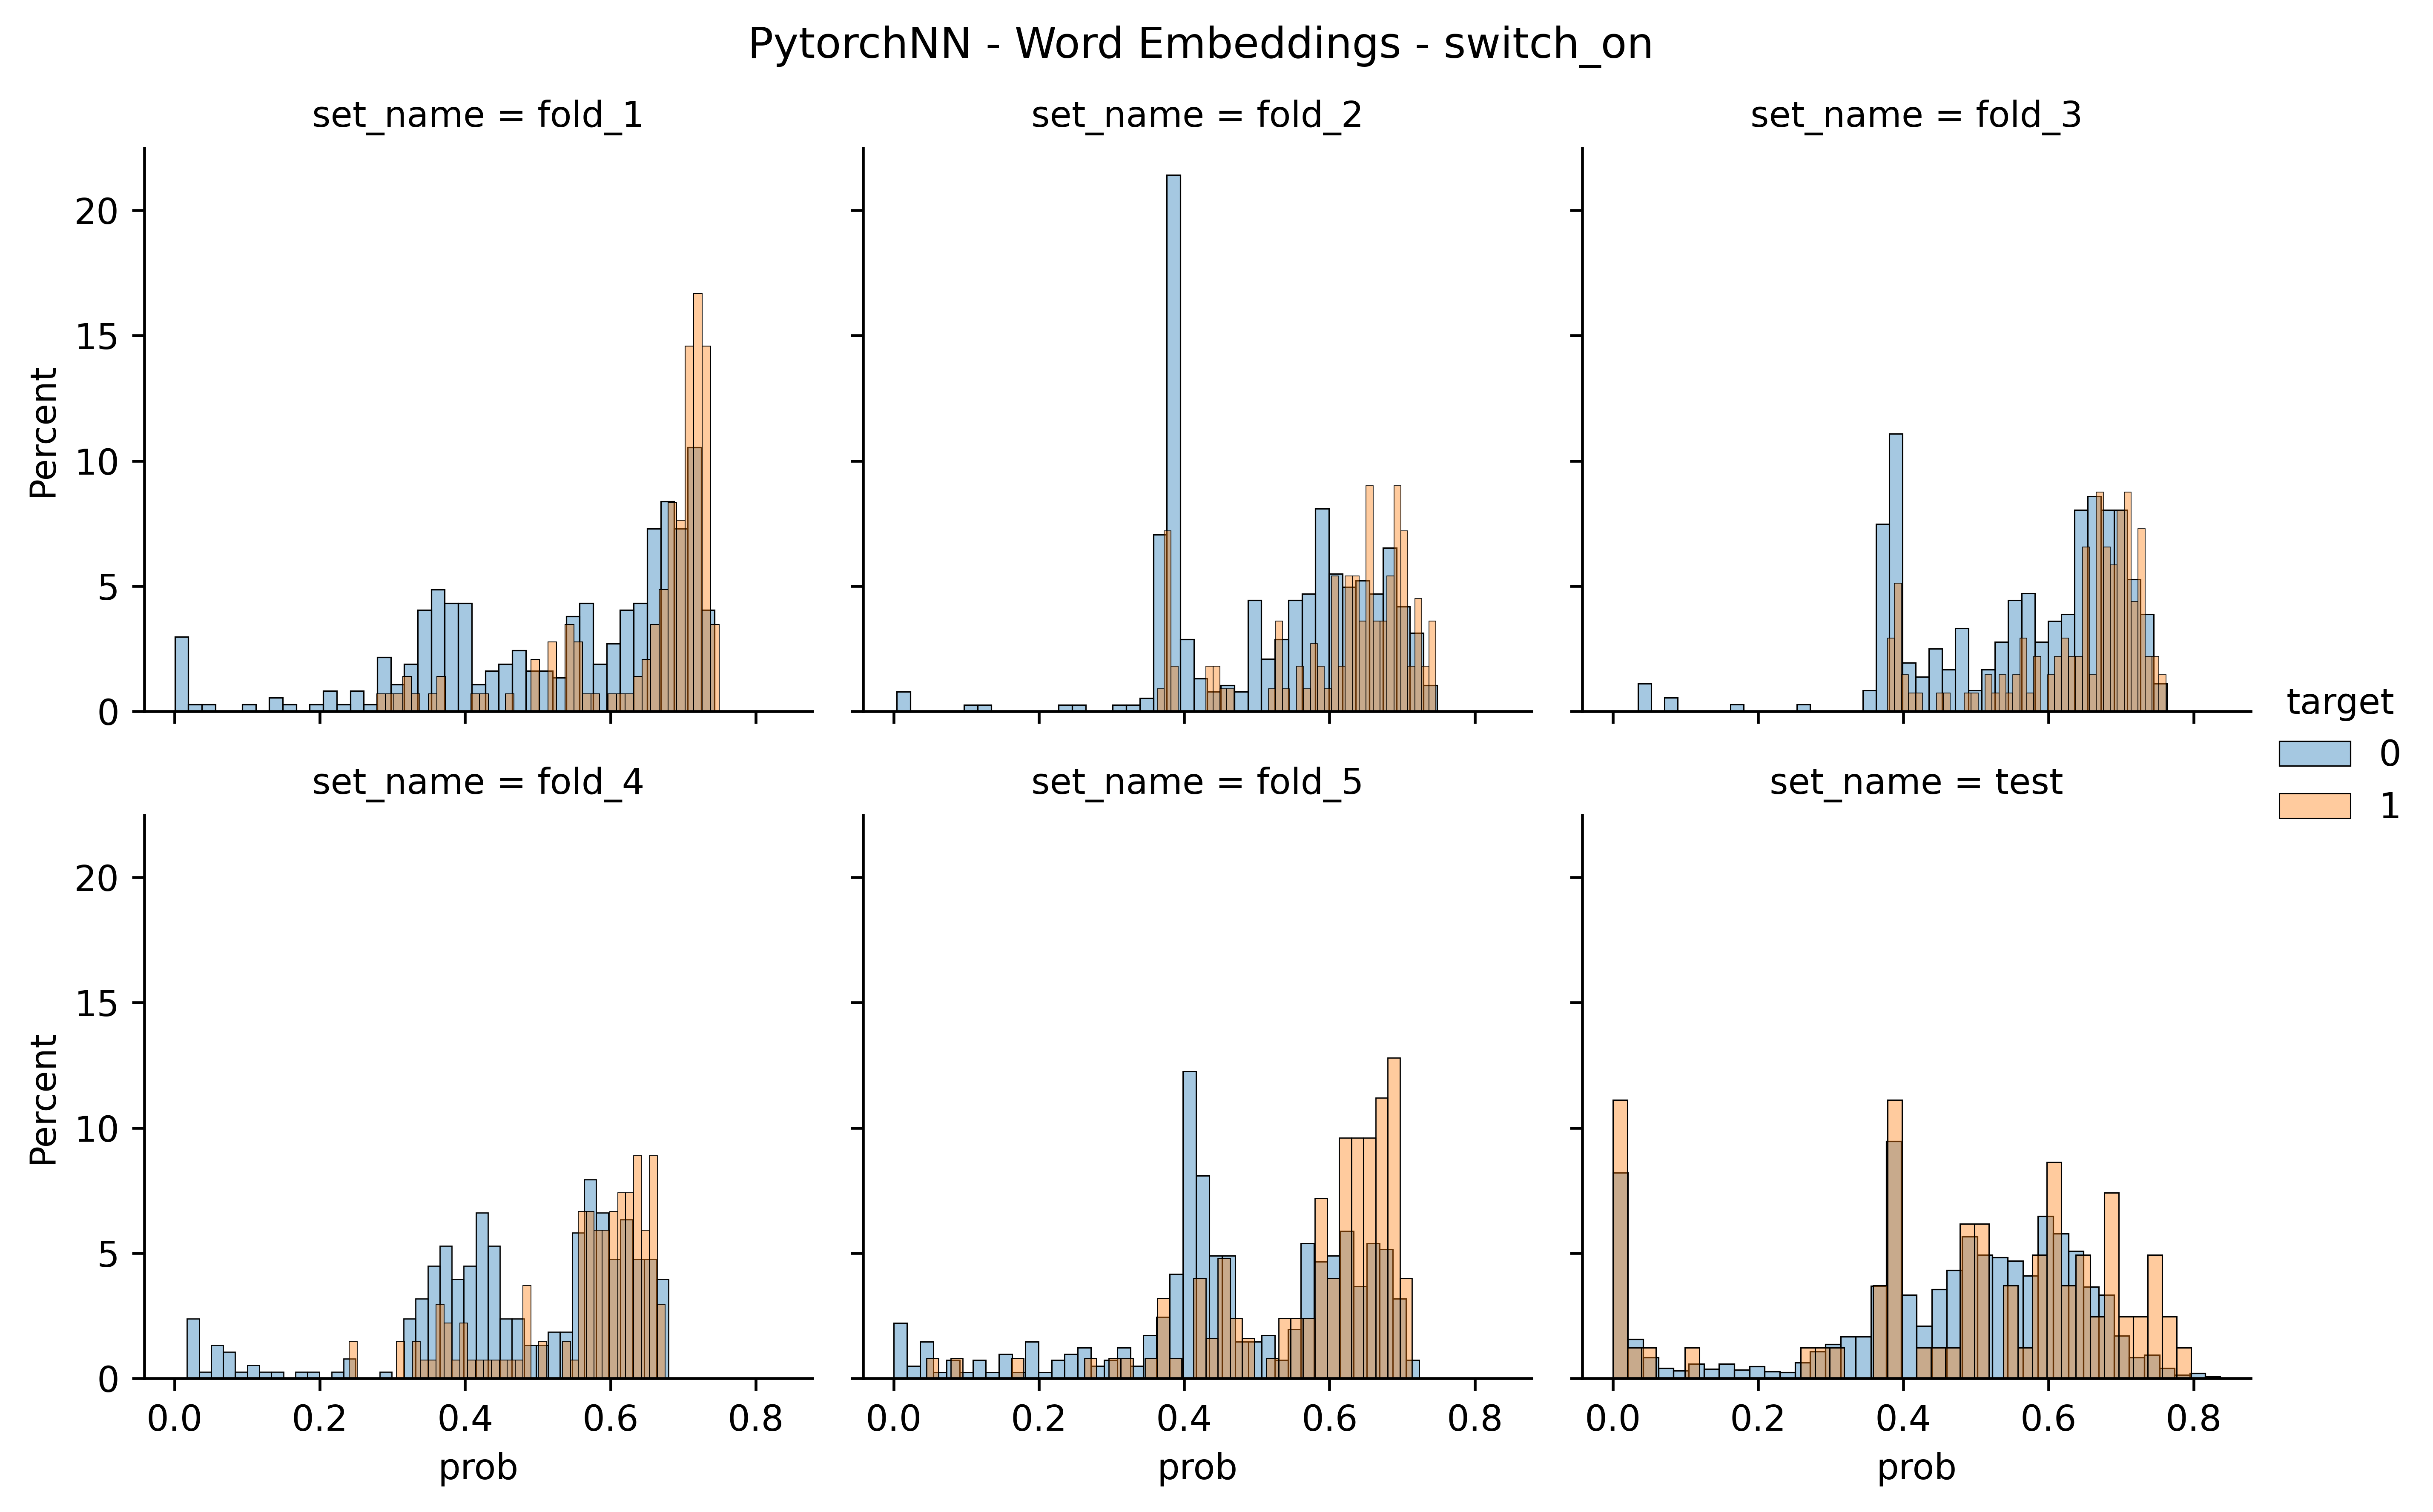
\includegraphics[width=\linewidth]{figures/results/word_embeddings/nn/switch_on/switch_on__distplot (1).png}
    \end{subfigure}
    \caption{Word embeddings switch\_on}
\end{figure}


\begin{figure}
    \begin{subfigure}[b]{\textwidth}
        \centering
        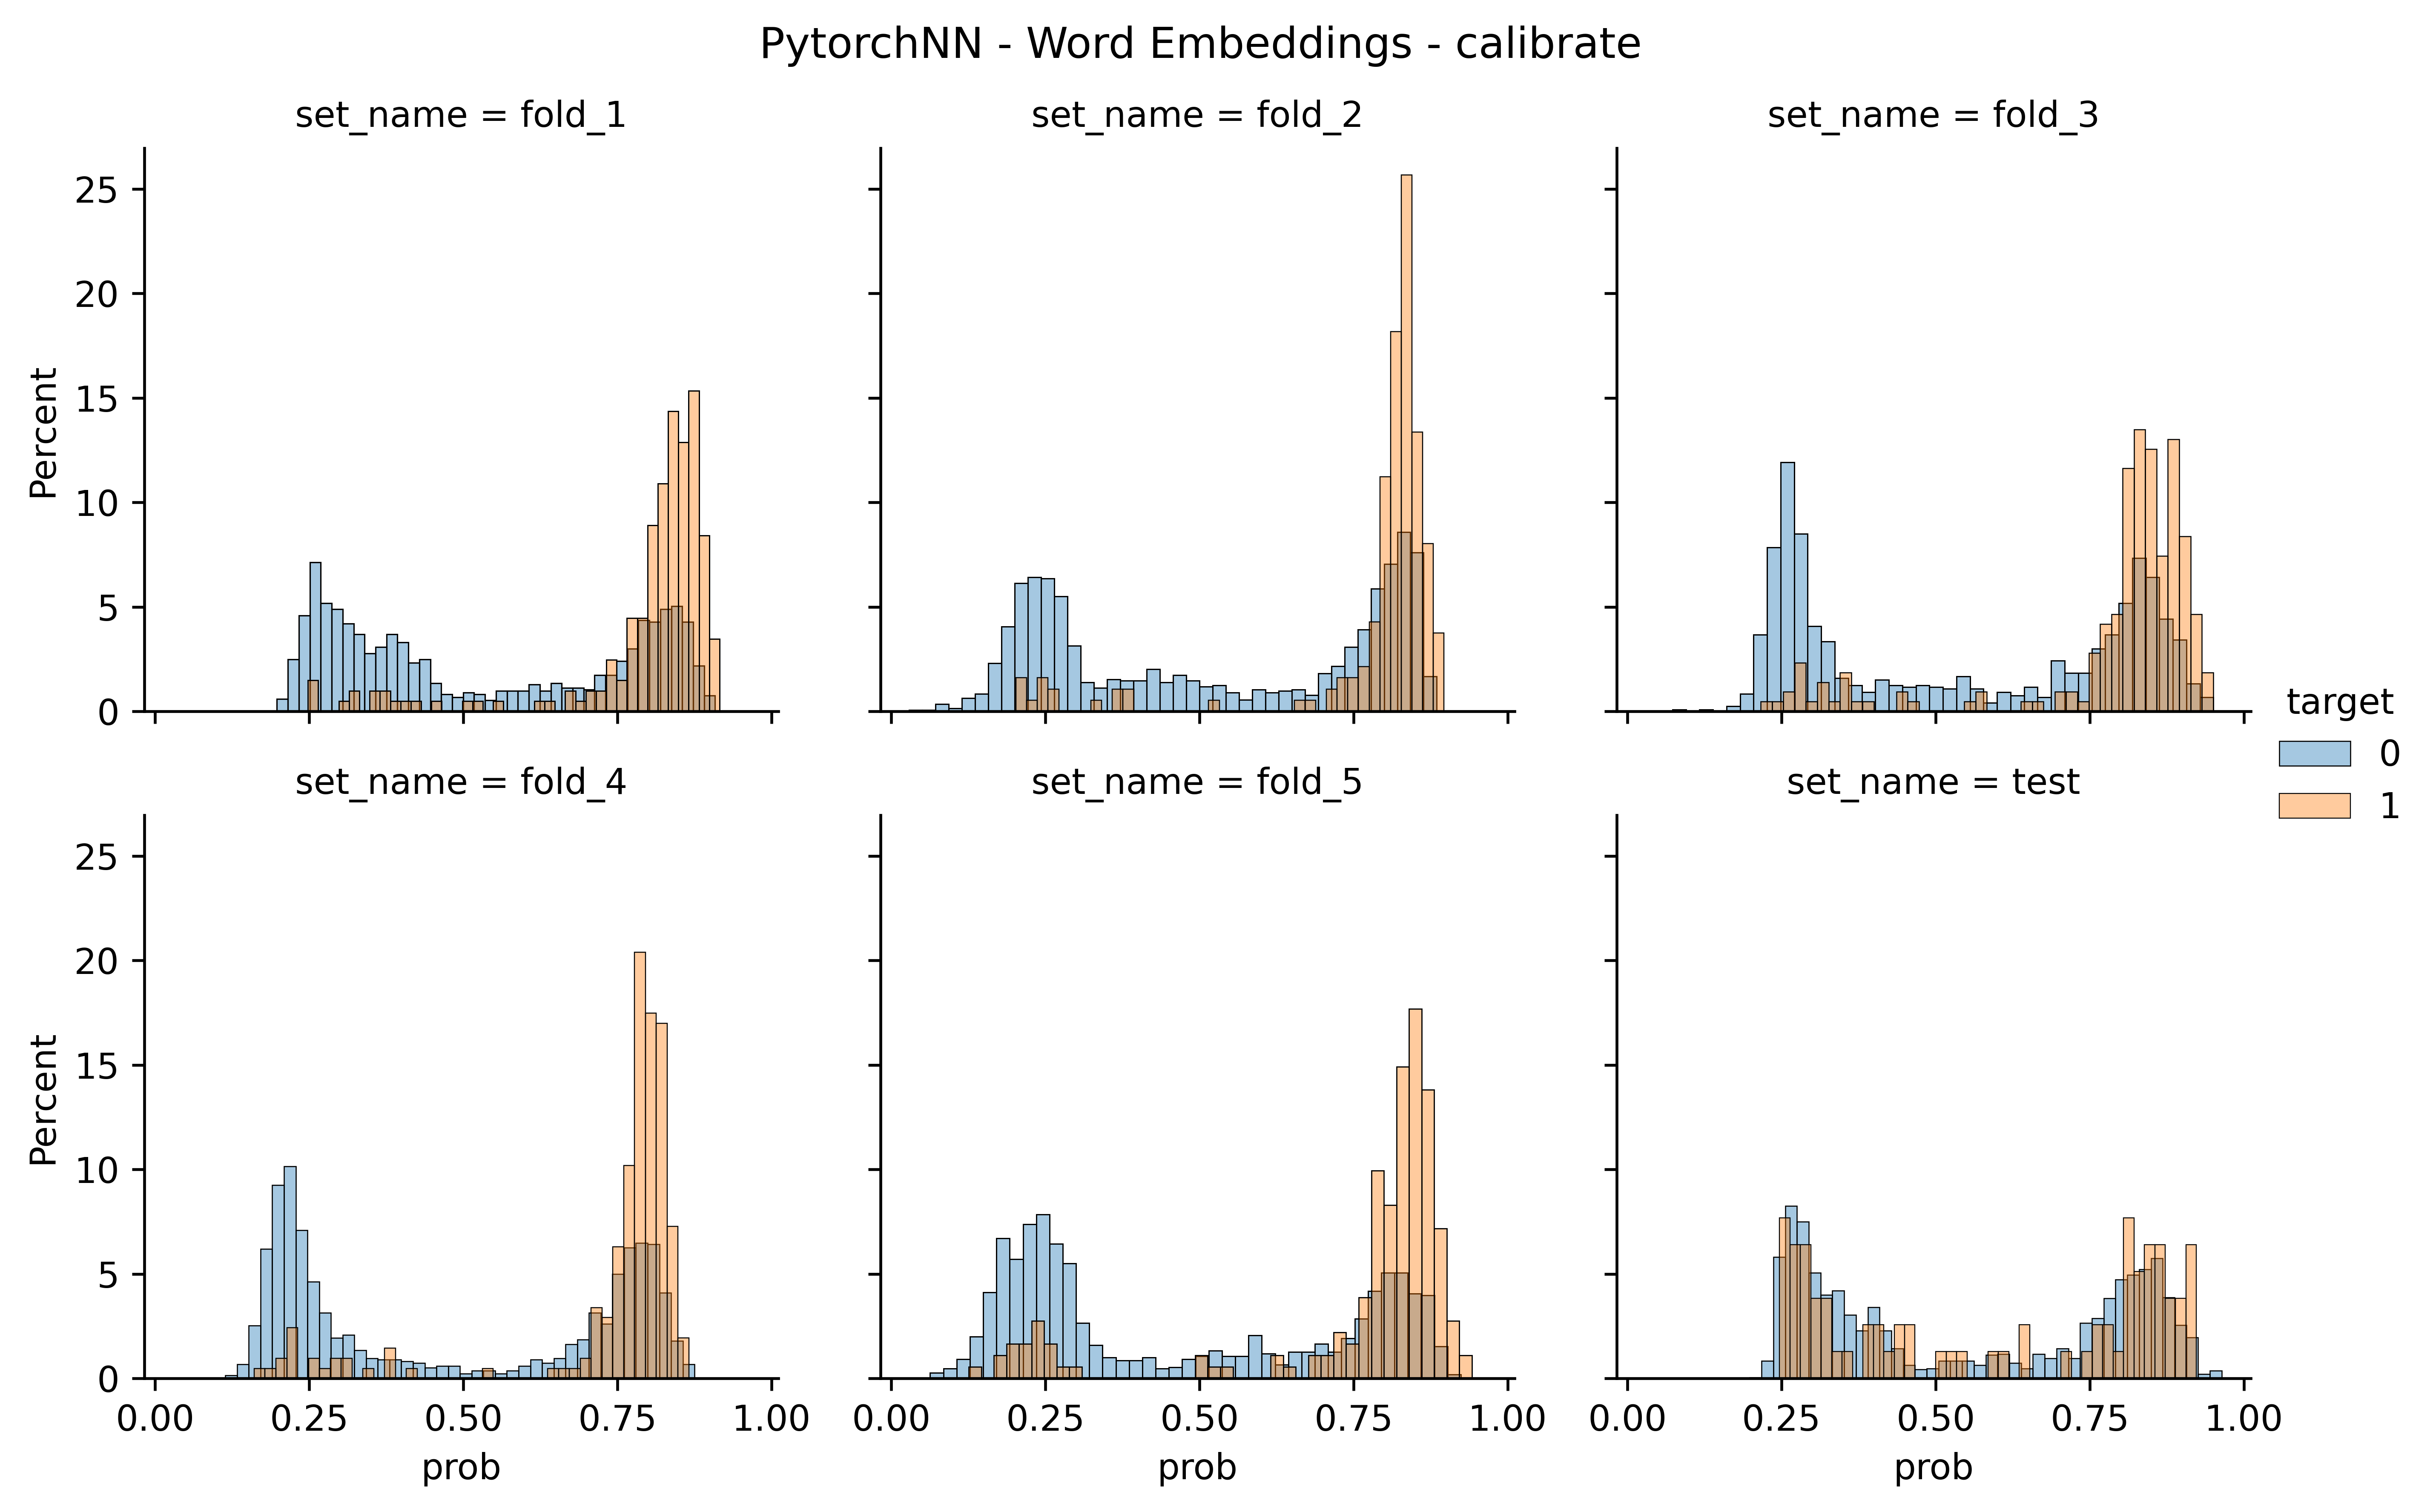
\includegraphics[width=\linewidth]{figures/results/word_embeddings/nn/calibrate/calibrate__distplot.png}
        \caption{Distribución de predicciones en validación cruzada y el conjunto de test.}
        \label{fig:my_label}
    \end{subfigure}
    \hfill
    \begin{subfigure}[b]{\textwidth}
    \minipage{0.32\textwidth}
      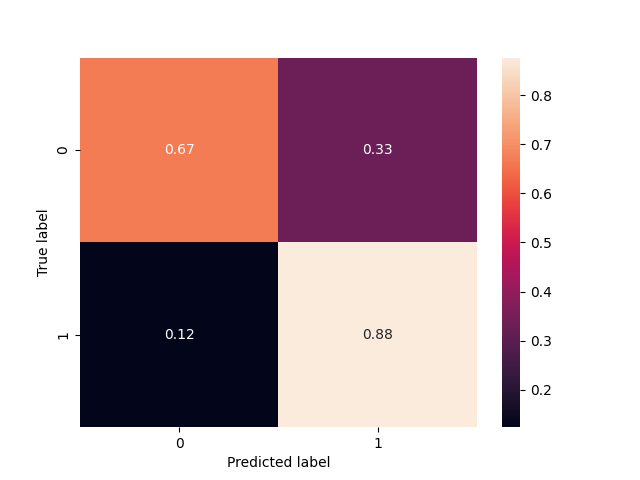
\includegraphics[width=\linewidth]{figures/results/word_embeddings/nn/calibrate/calibrate_set_1_confusion_matrix_percent.png}
    \endminipage\hfill
    \minipage{0.32\textwidth}
      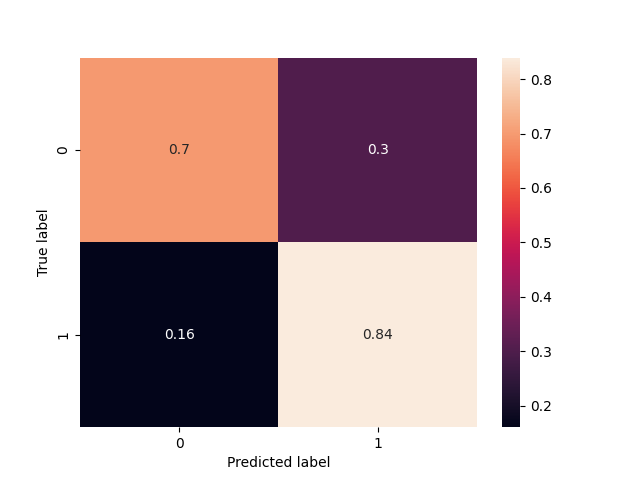
\includegraphics[width=\linewidth]{figures/results/word_embeddings/nn/calibrate/calibrate_set_2_confusion_matrix_percent.png}
    \endminipage\hfill \minipage{0.32\textwidth}%
      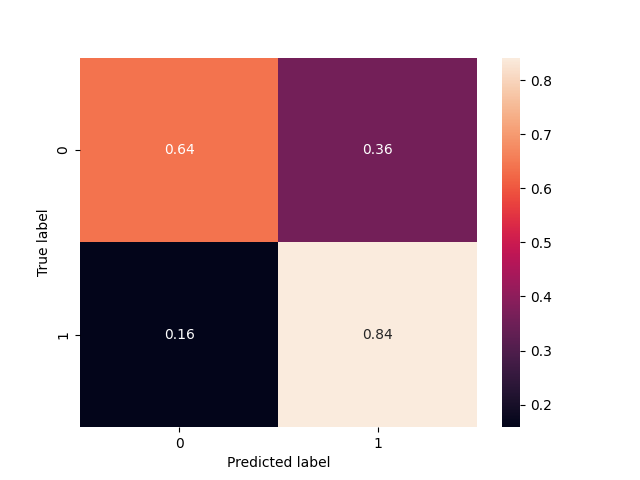
\includegraphics[width=\linewidth]{figures/results/word_embeddings/nn/calibrate/calibrate+_set_3_confusion_matrix_percent.png}
    \endminipage
    
    \medskip
    
    \minipage{0.32\textwidth}
      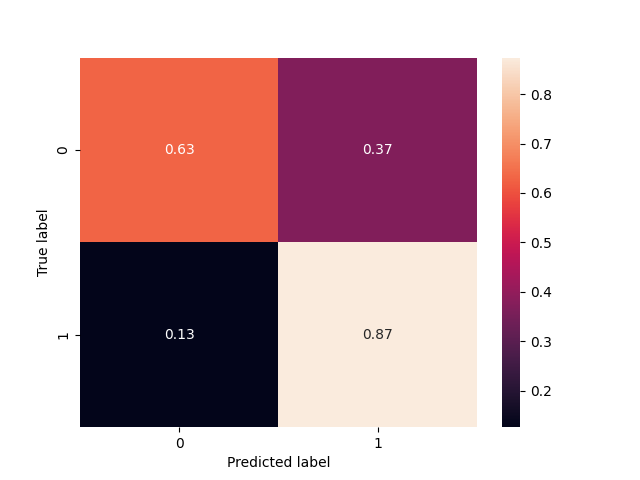
\includegraphics[width=\linewidth]{figures/results/word_embeddings/nn/calibrate/calibrate_set_4_confusion_matrix_percent.png}
    \endminipage\hfill
    \minipage{0.32\textwidth}
    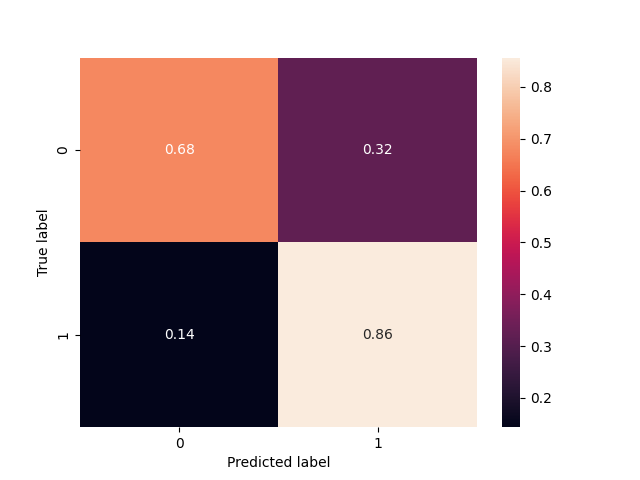
\includegraphics[width=\linewidth]{figures/results/word_embeddings/nn/calibrate/calibrate_set_5_confusion_matrix_percent.png}
    \endminipage\hfill \minipage{0.32\textwidth}%
    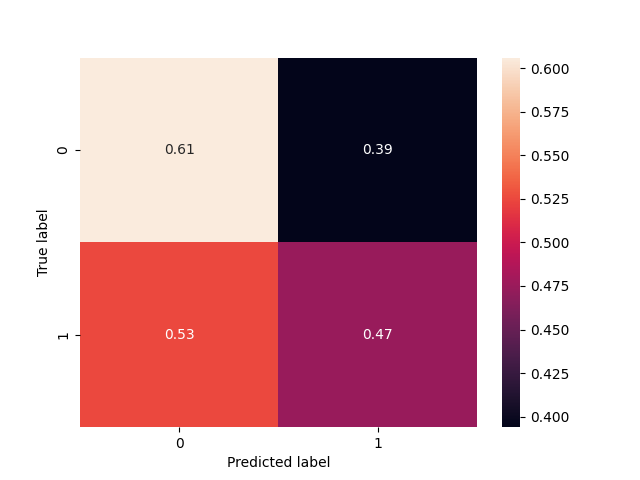
\includegraphics[width=\linewidth]{figures/results/word_embeddings/nn/calibrate/calibrate_set_6_confusion_matrix_percent.png}
    \endminipage
    \caption{Matrices de confusión en validación cruzada y el conjunto de test}
    \end{subfigure}
    \caption{Resultados del modelo de redes neuronales con codificación por word embeddings y esquema de acción calibrate.}
\end{figure}

\begin{table}[h!]
\centering
\scalebox{0.9}{
 \begin{tabular}{|c || c | c | c | c | c | c |} 
 \hline
  Esquemas & Precisión & Recall & $H_{1.5}$ & $F_{1.5}$ & Umbral de decisión &
  Modelo \\
 \hline
 take\_image & 0.8088 & 0.997 & 0.4351 & 0.997 & 0.61 & LGR \\
 calibrate & 0.0467 & 0.4743 & 0.5083 & 0.1242 & 0.728 & NN\\
 switch\_on  & 0.0405 & 0.4567 & 0.5106 & 0.1097 & 0.576 & NN\\
 switch\_off & 0.0476 & 0.1818 & 0.2422 & 0.0876 & 0.034 & NN \\
 turn\_to  & - & - & - & - & - & -\\[1ex]
 \hline
 \end{tabular}}
 \caption{Resultados por esquema de acción del mejor modelo con codificación por word embeddings.}
 \label{results:ad-hoc-calibrate}
\end{table}


\section{Modelos predictivos ad-hoc}
\label{exp:wb}

\subsection{Configuración del experimento}

Como contraparte del experimento anterior, usaremos la codificación por word
embeddings, bajo el mismo conjunto de entrenamientos y construcción de ventanas,
con la salvedad de ser codificados a partir del modelo de lenguaje de FastText,
entrenado con oraciones provenientes de planes relajados. El modelo de lenguaje
es un modelo Skipgram entrenado por $100$ épocas, un tamaño de ventana de
contexto de $3$ palabras, y un vector de salida de dimensión $30$. Se hicieron
pruebas sobre otras configuraciones de parámetros pero el comportamiento que
buscábamos que el modelo de lenguaje aprendiese ya era obtenido bajo esta
configuración.

Los clasificadores y grillas de búsqueda de parámetros utilizadas fueron las
mismos que los modelo predictivos ad-hoc.

\subsection{Resultados}

\begin{figure}
    \centering
    \begin{subfigure}[b]{0.83\textwidth}
    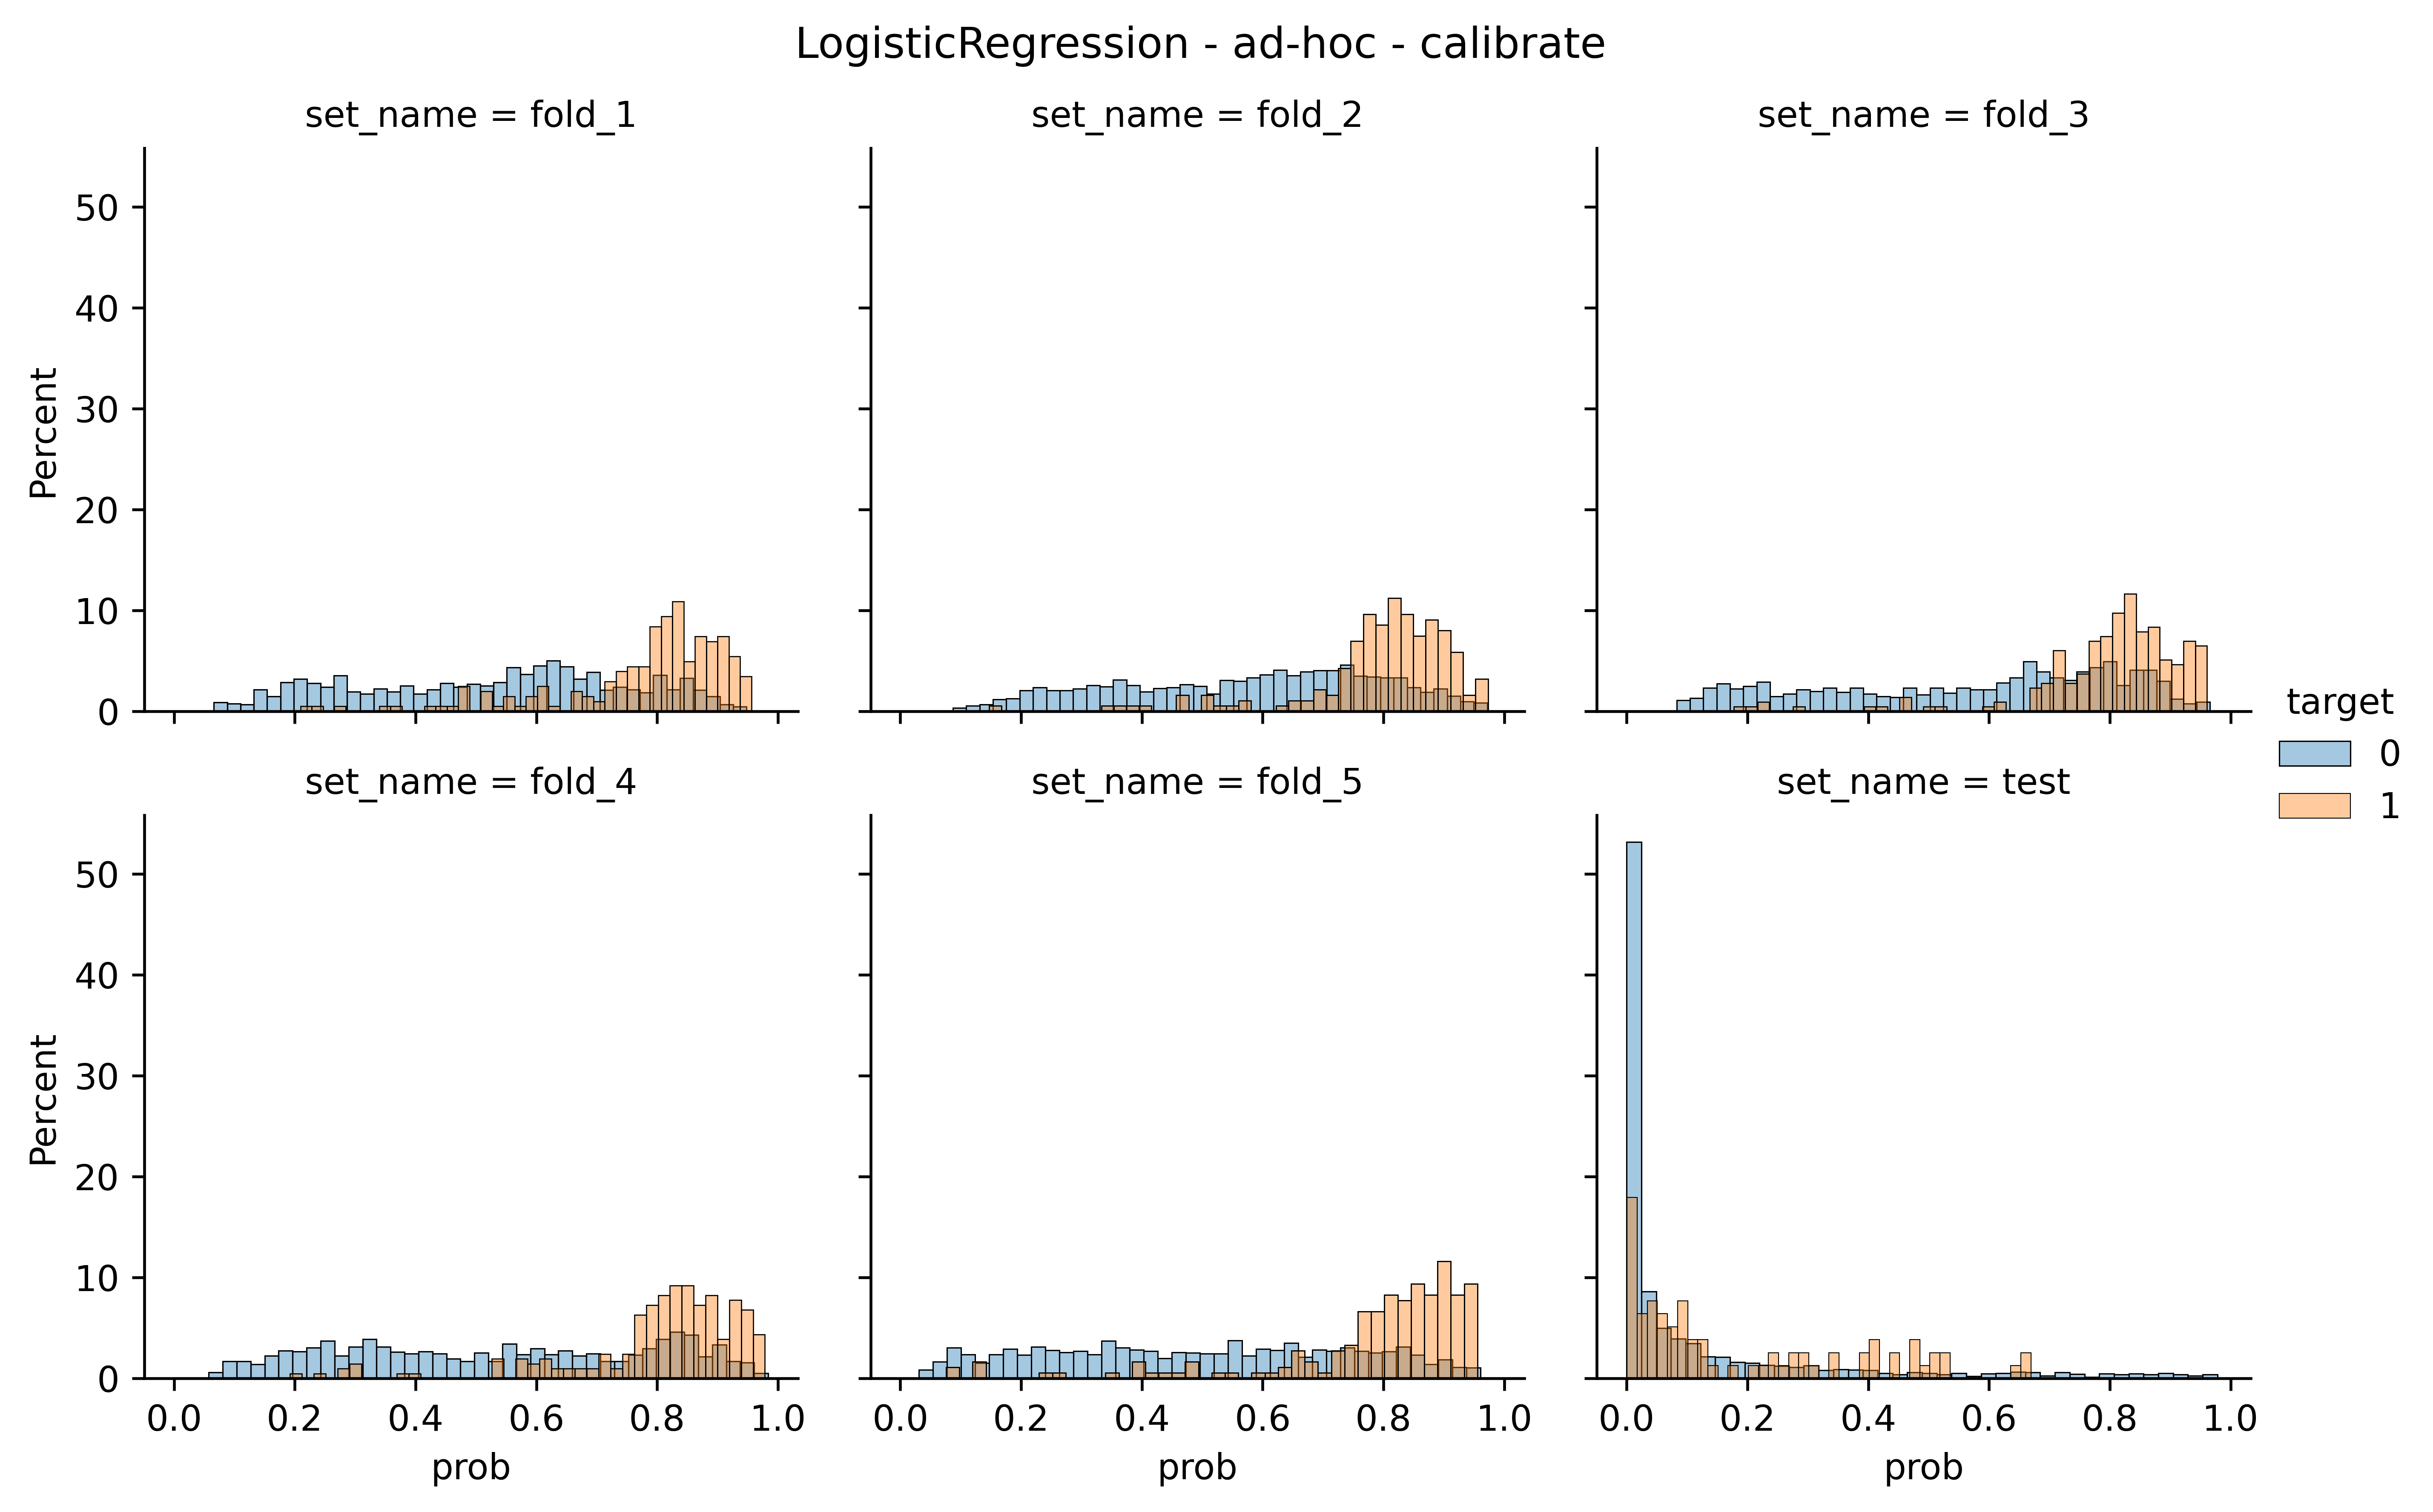
\includegraphics[width=\linewidth]{figures/results/ad-hoc/lgr/calibrate/calibrate__distplot.png}
    \end{subfigure}
    \hfill
    \centering
    \begin{subfigure}[b]{0.83\textwidth}
        \centering
        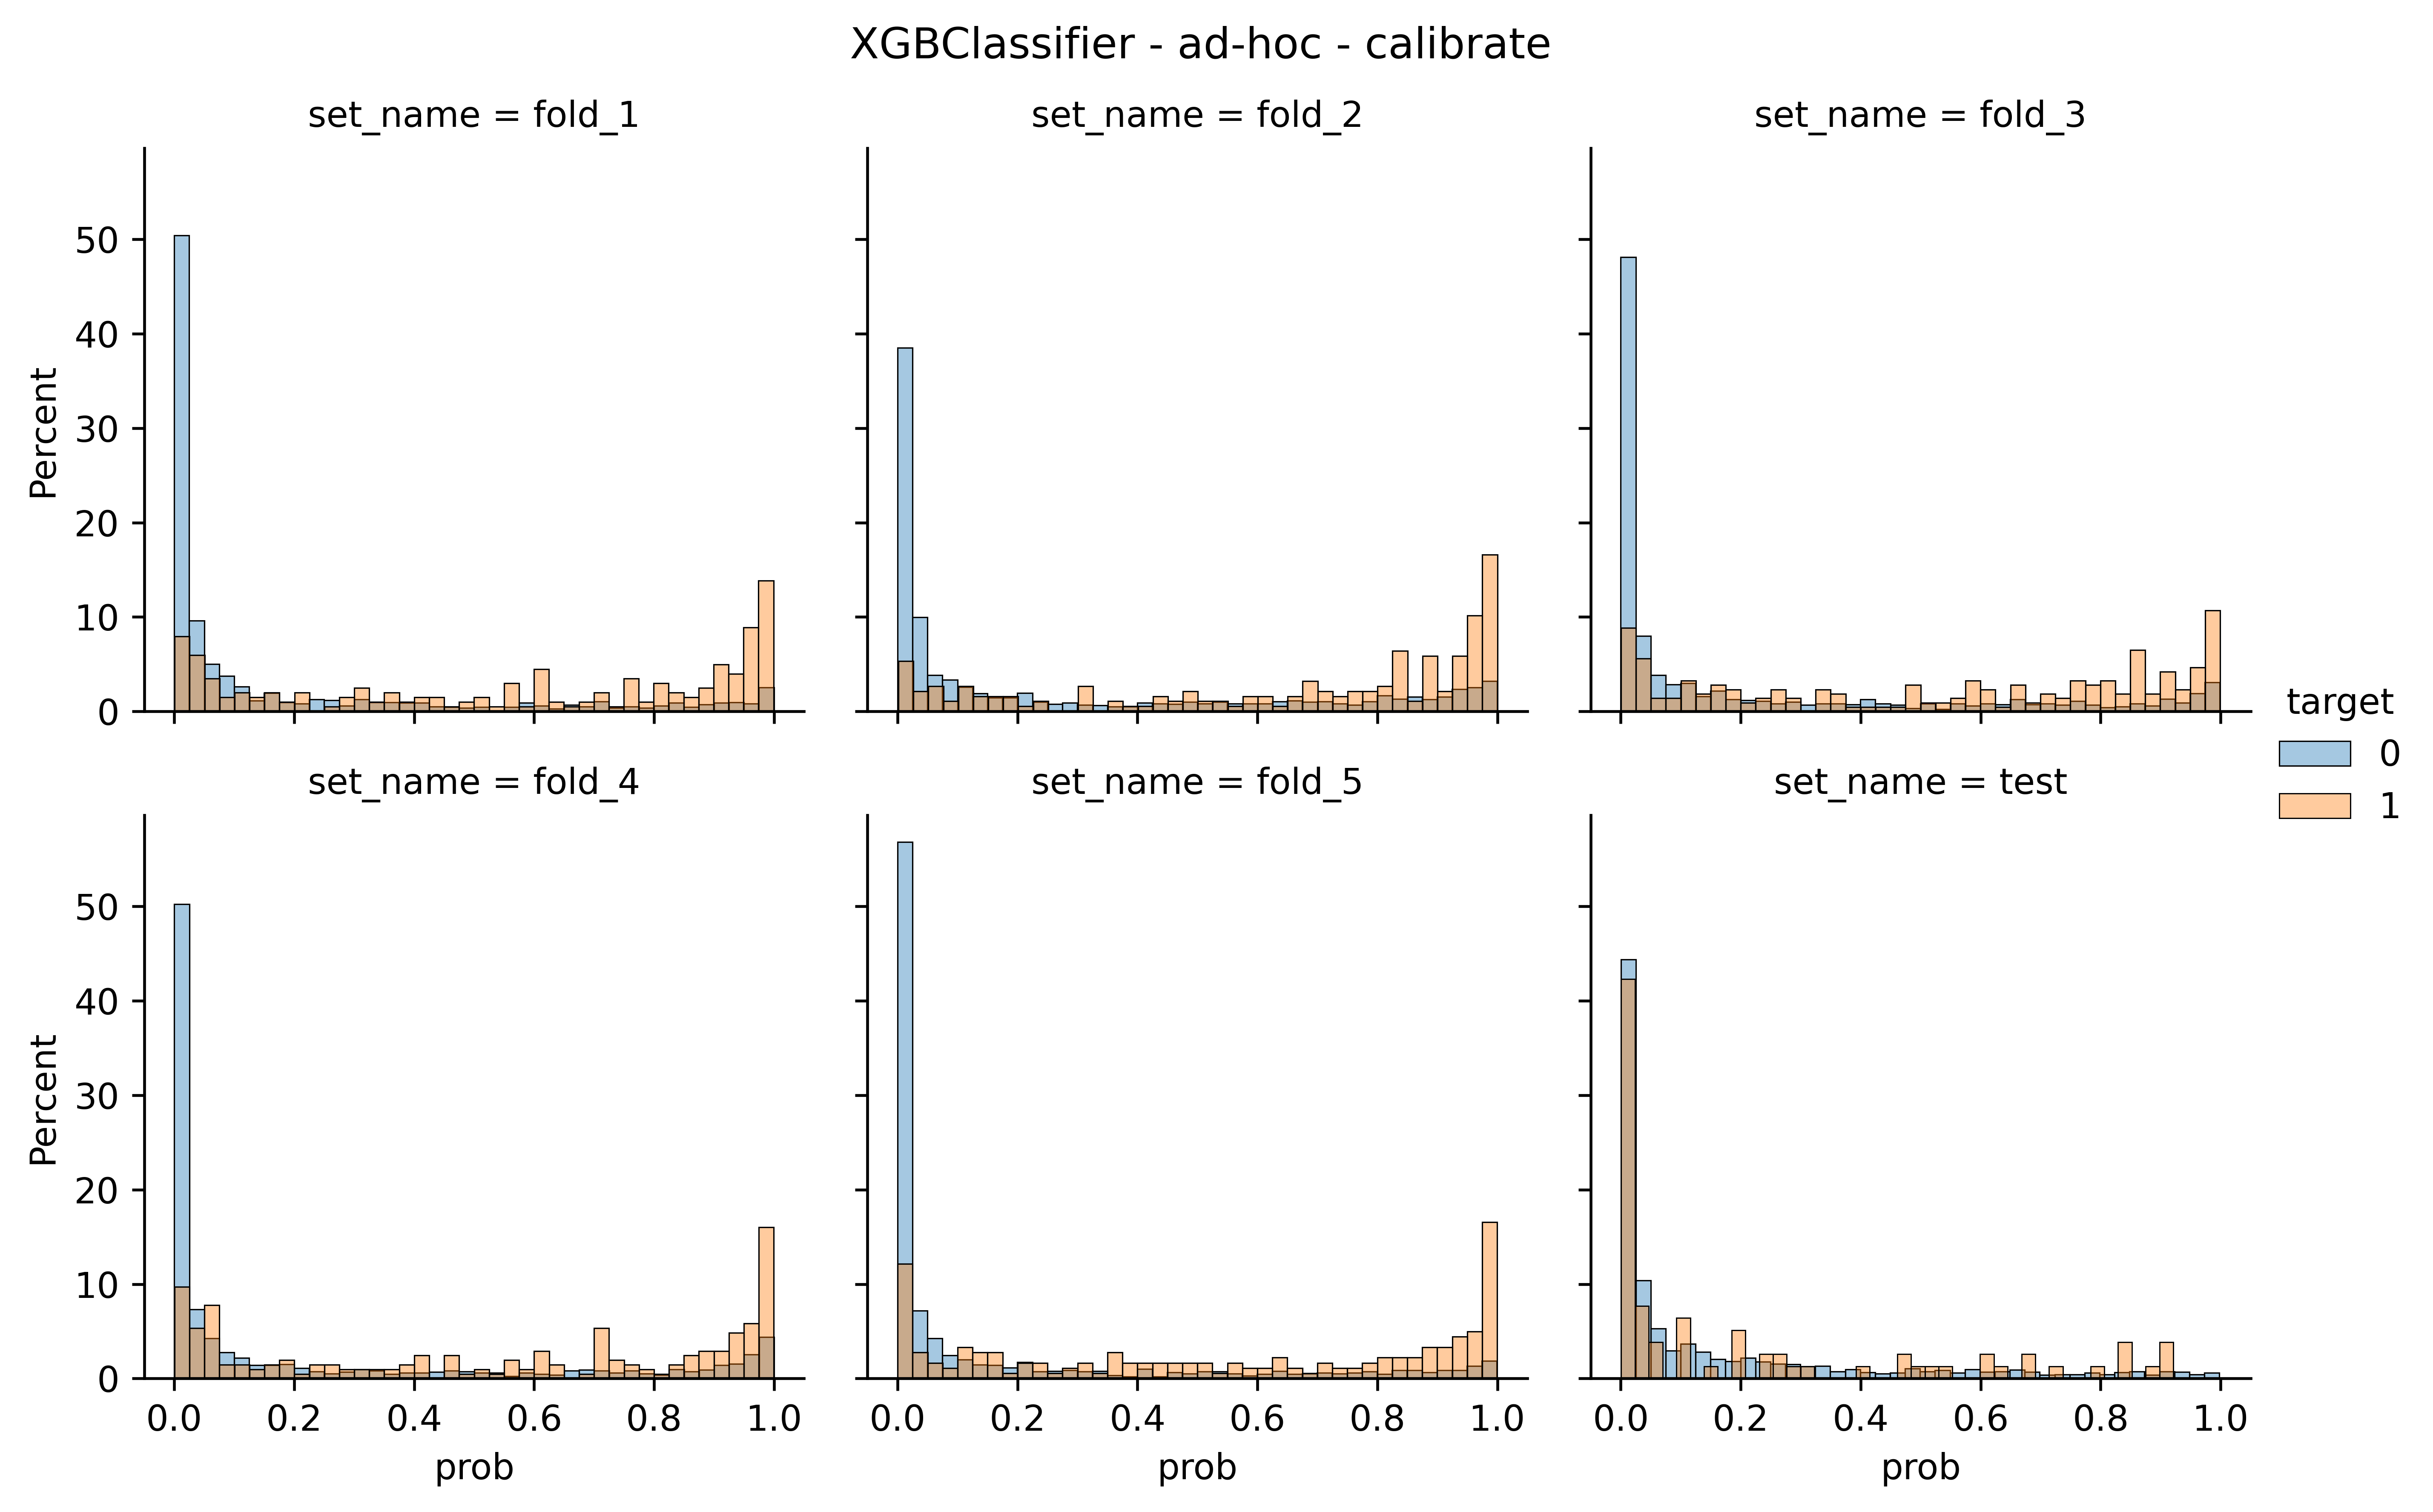
\includegraphics[width=\linewidth]{figures/results/ad-hoc/xgb/2021-12-07_06.29.19.600877__distplot (2).png}
    \end{subfigure}
    \hfill
    \centering
    \begin{subfigure}[b]{0.83\textwidth}
        \centering
        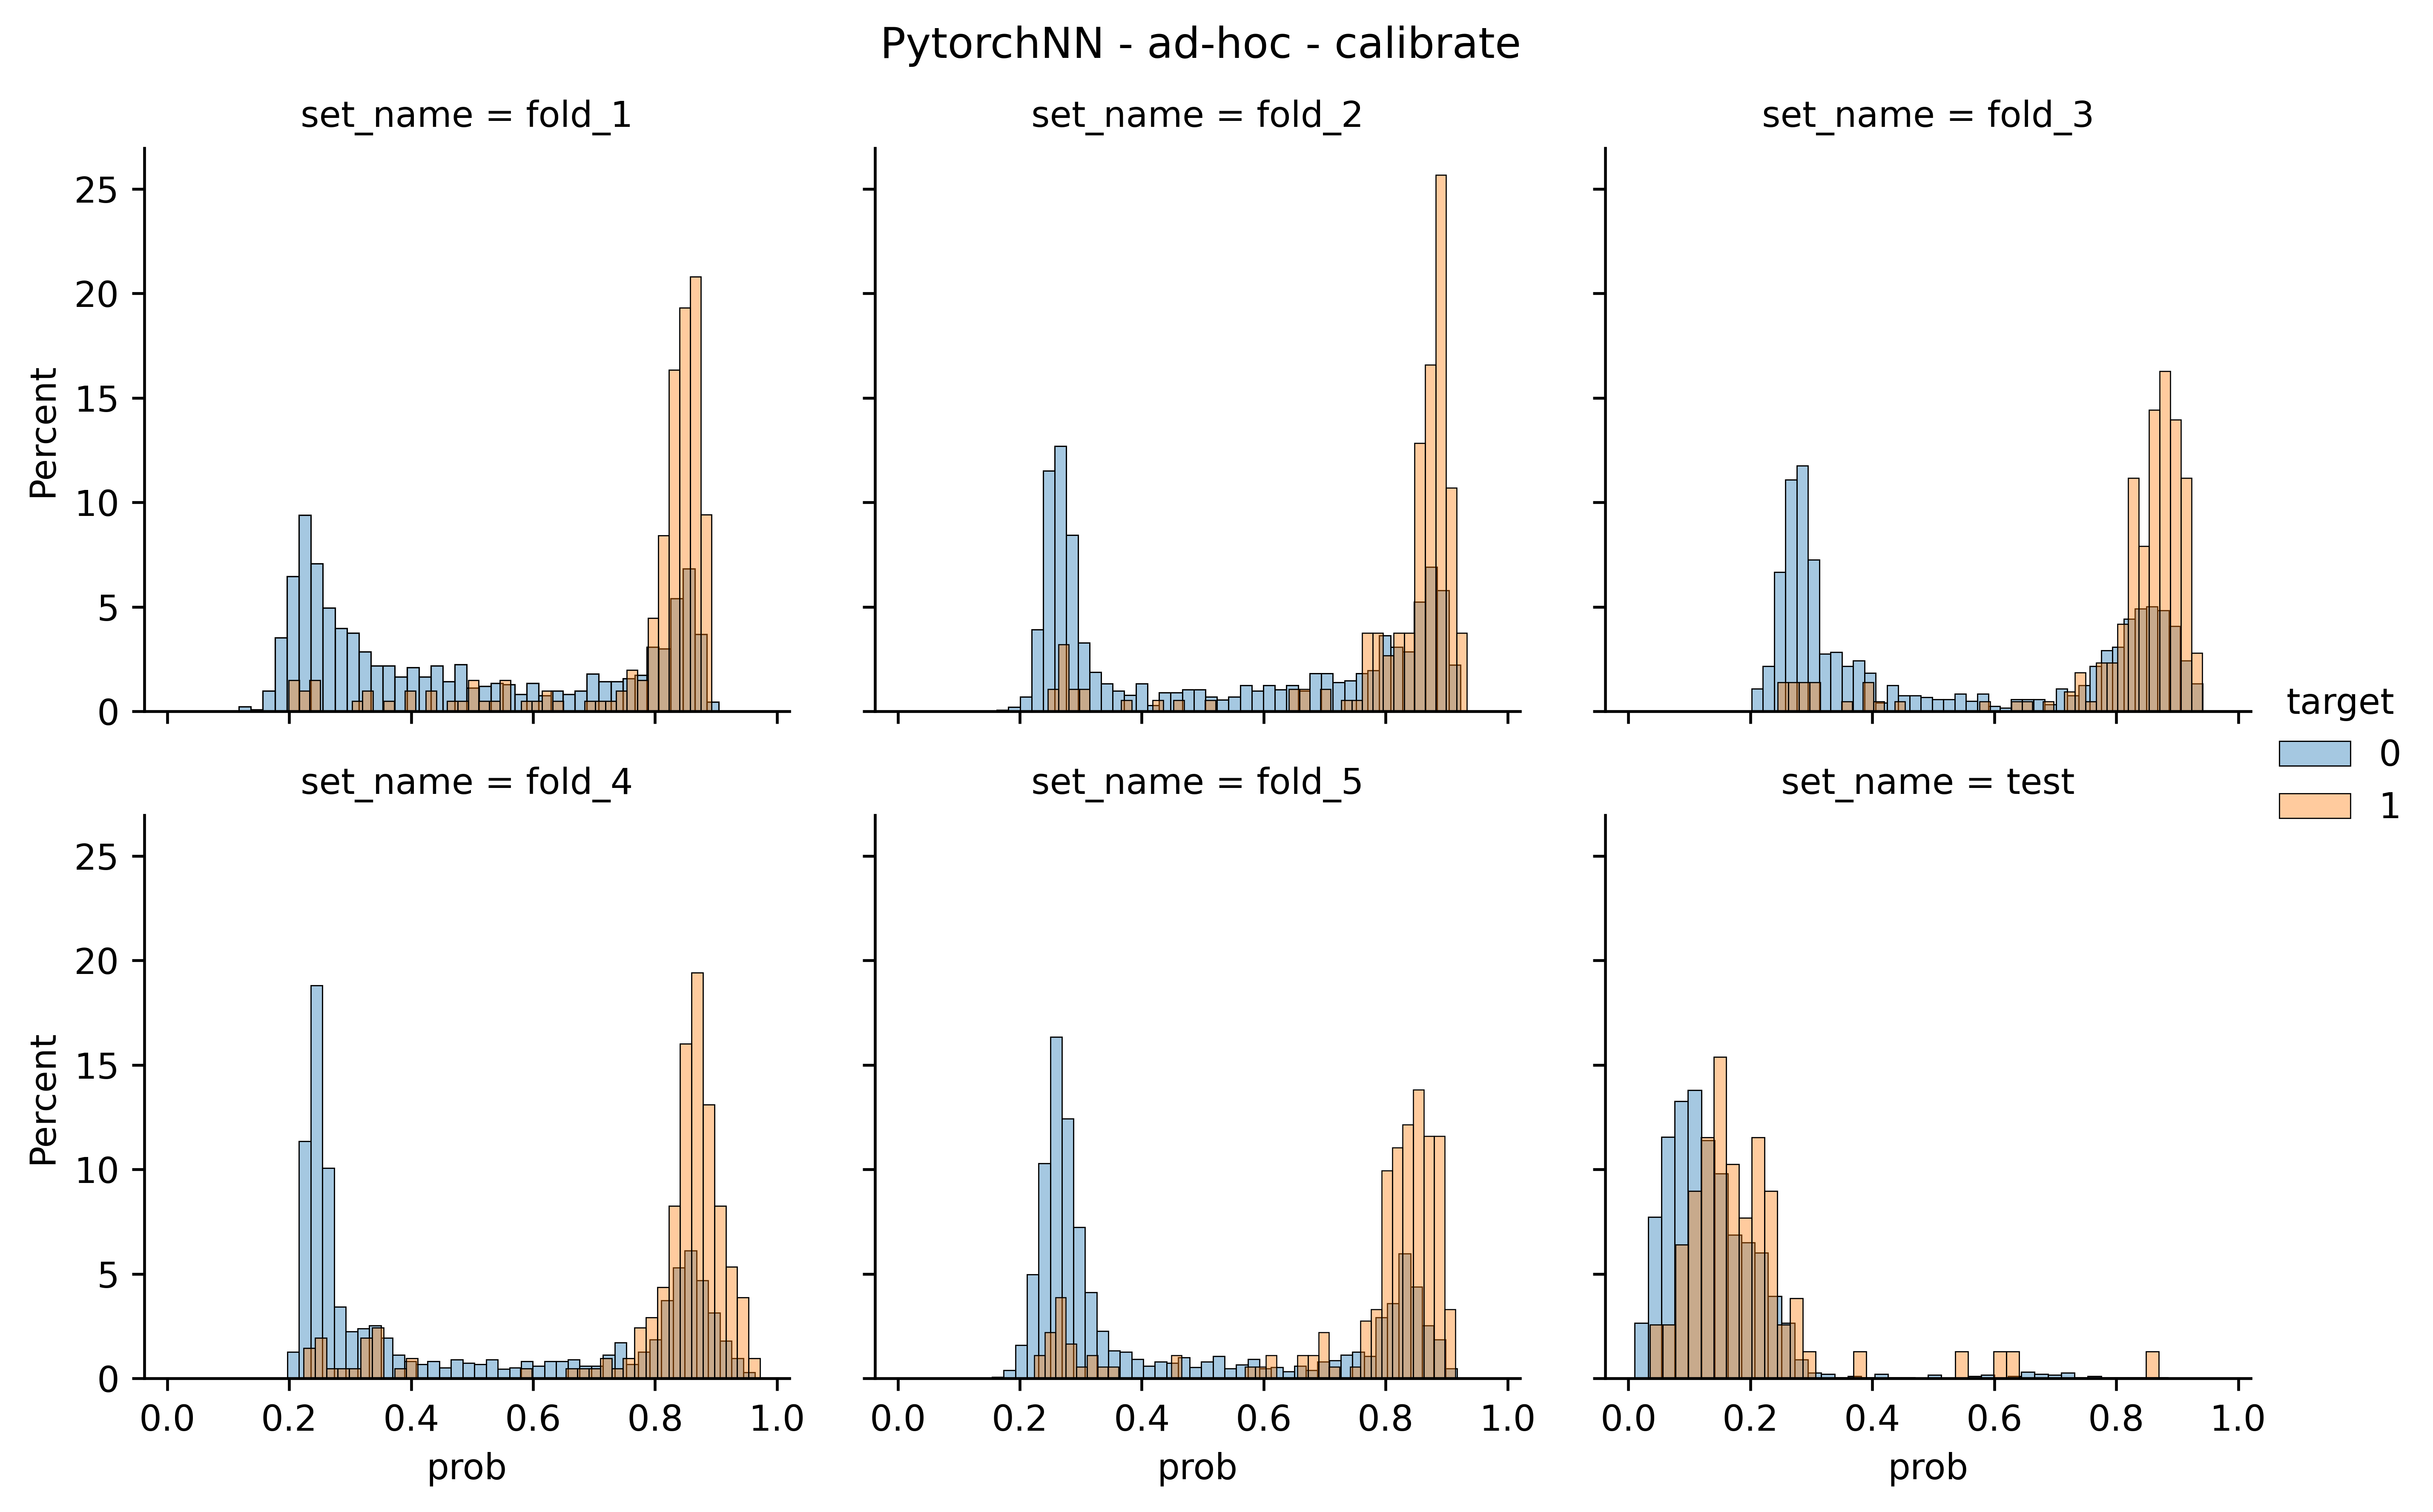
\includegraphics[width=\linewidth]{figures/results/ad-hoc/nn/2021-12-06_17.03.17.314982__distplot.png}
    \end{subfigure}
    \caption{Ad-hoc calibrate}
\end{figure}

\begin{figure}
    \centering
    \begin{subfigure}[b]{0.83\textwidth}
    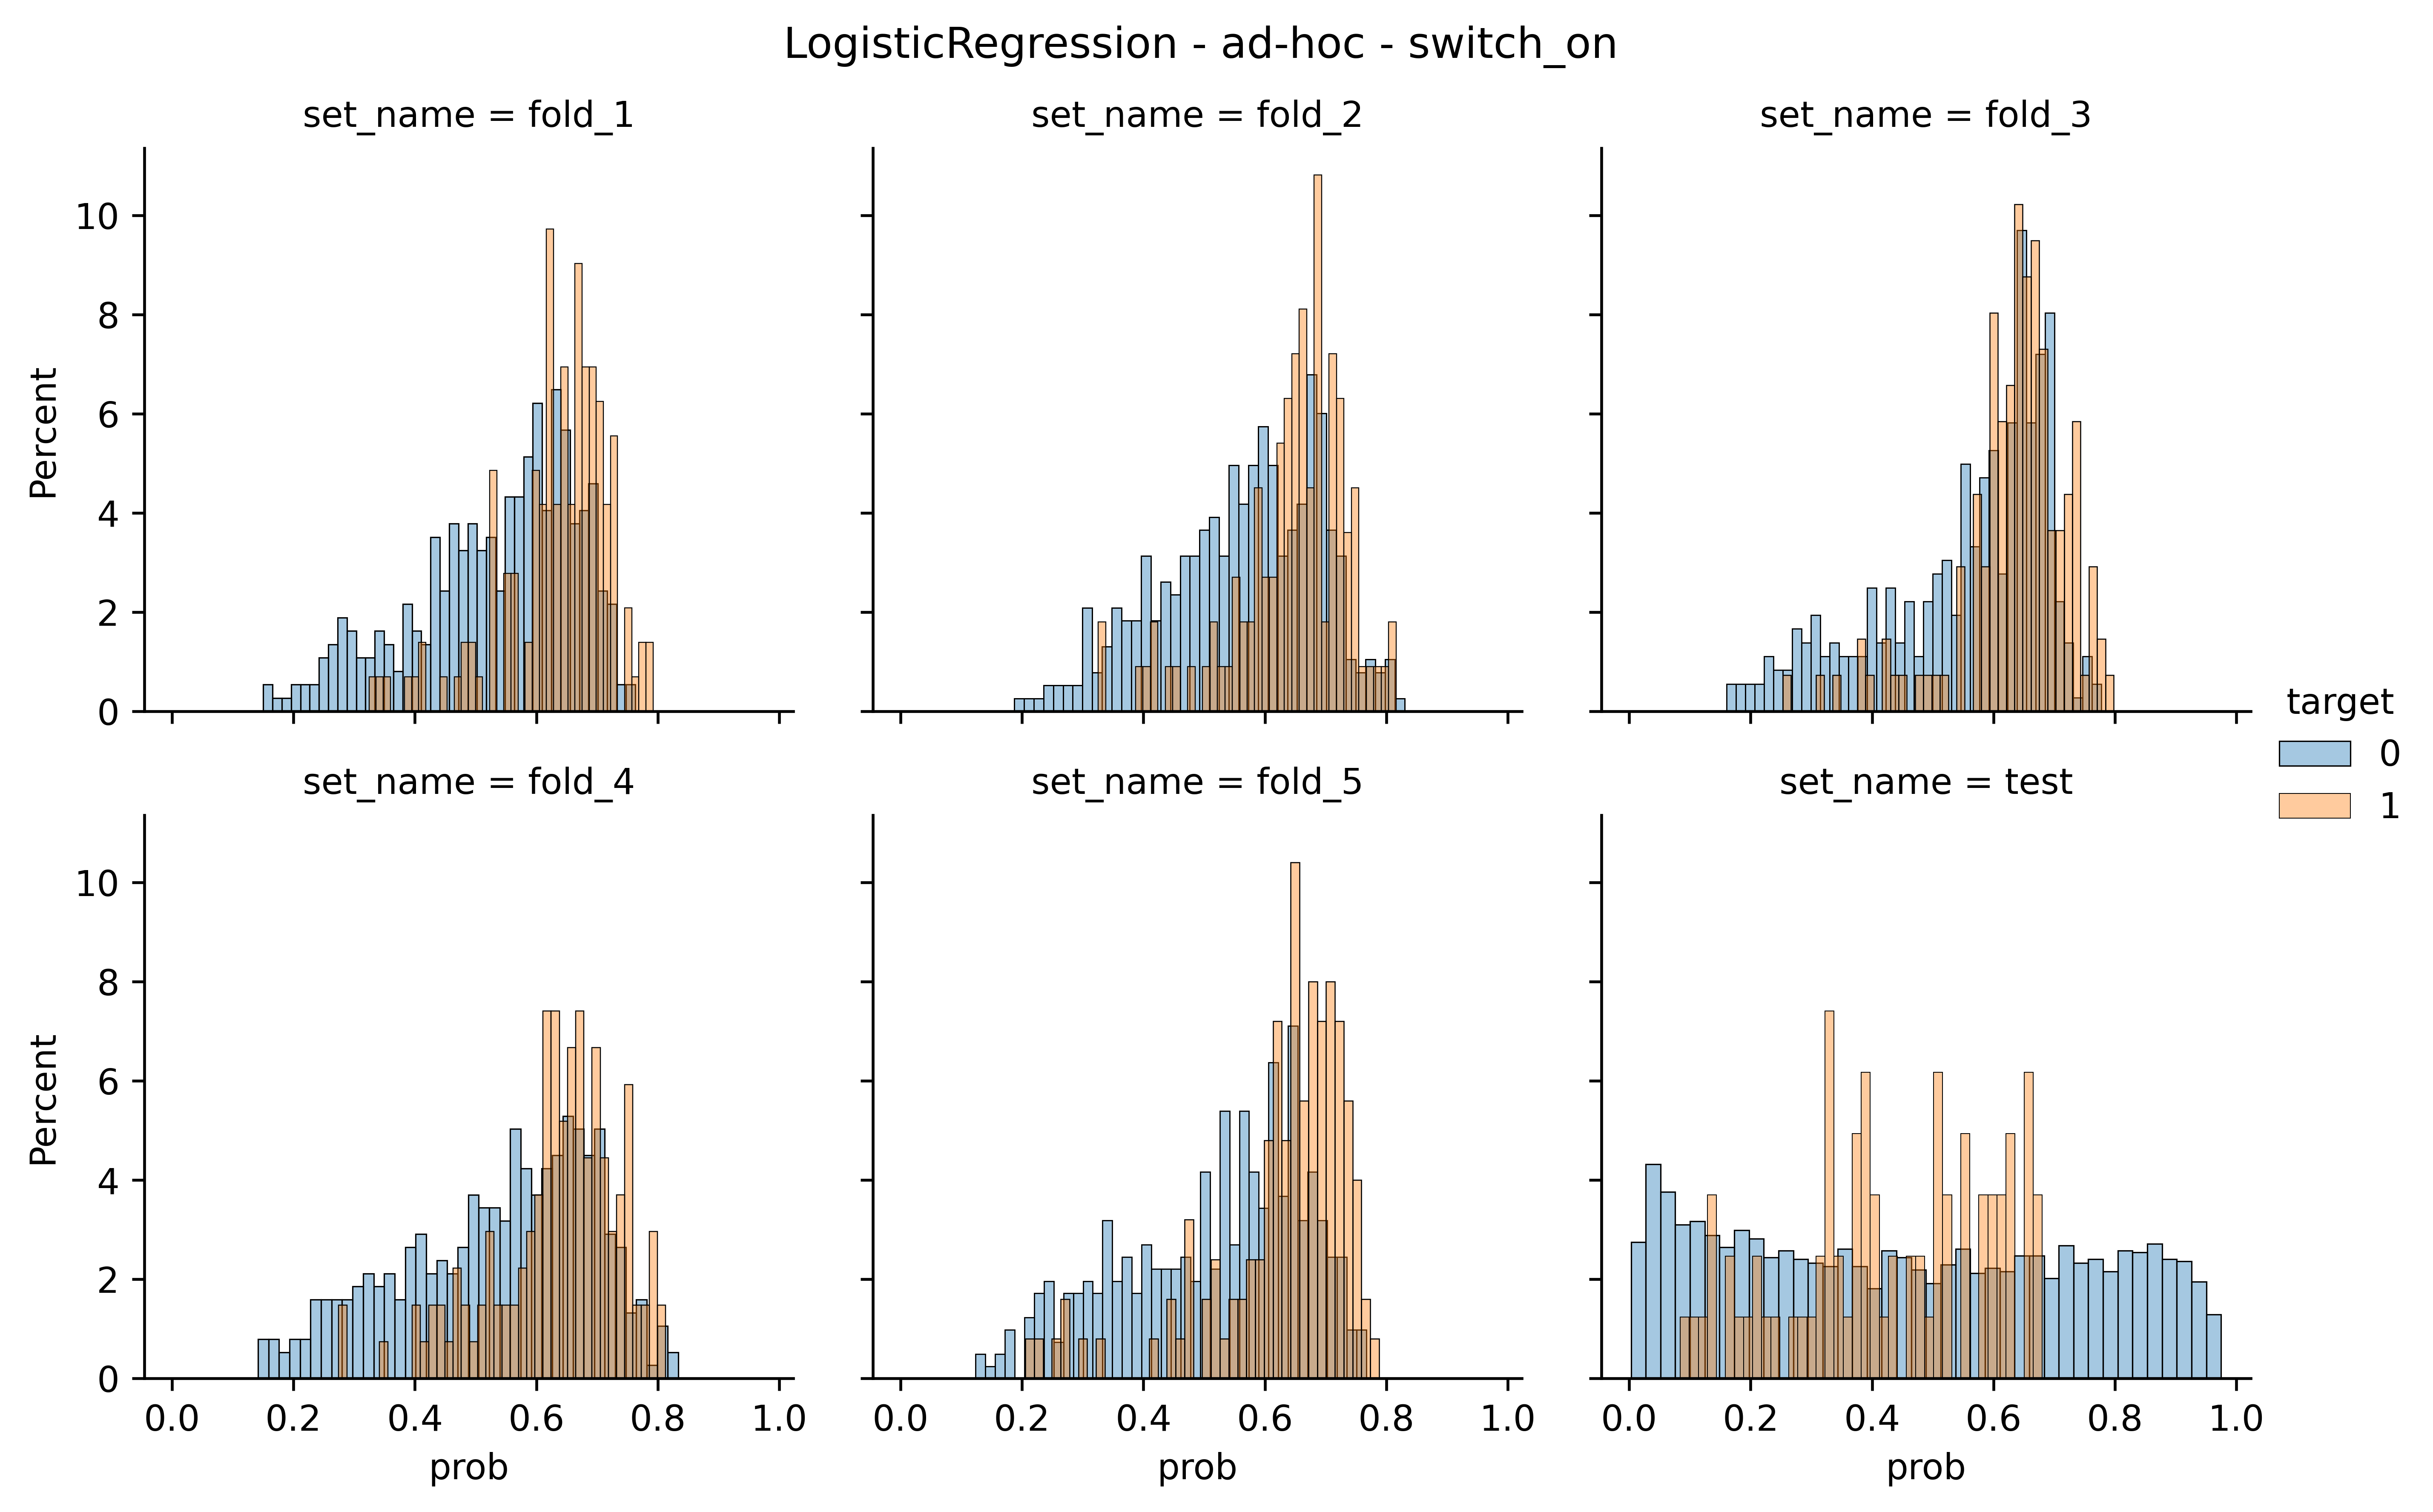
\includegraphics[width=\linewidth]{figures/results/ad-hoc/lgr/switch_on/turn_to__distplot.png}
    \end{subfigure}
    \hfill
    \centering
    \begin{subfigure}[b]{0.83\textwidth}
        \centering
        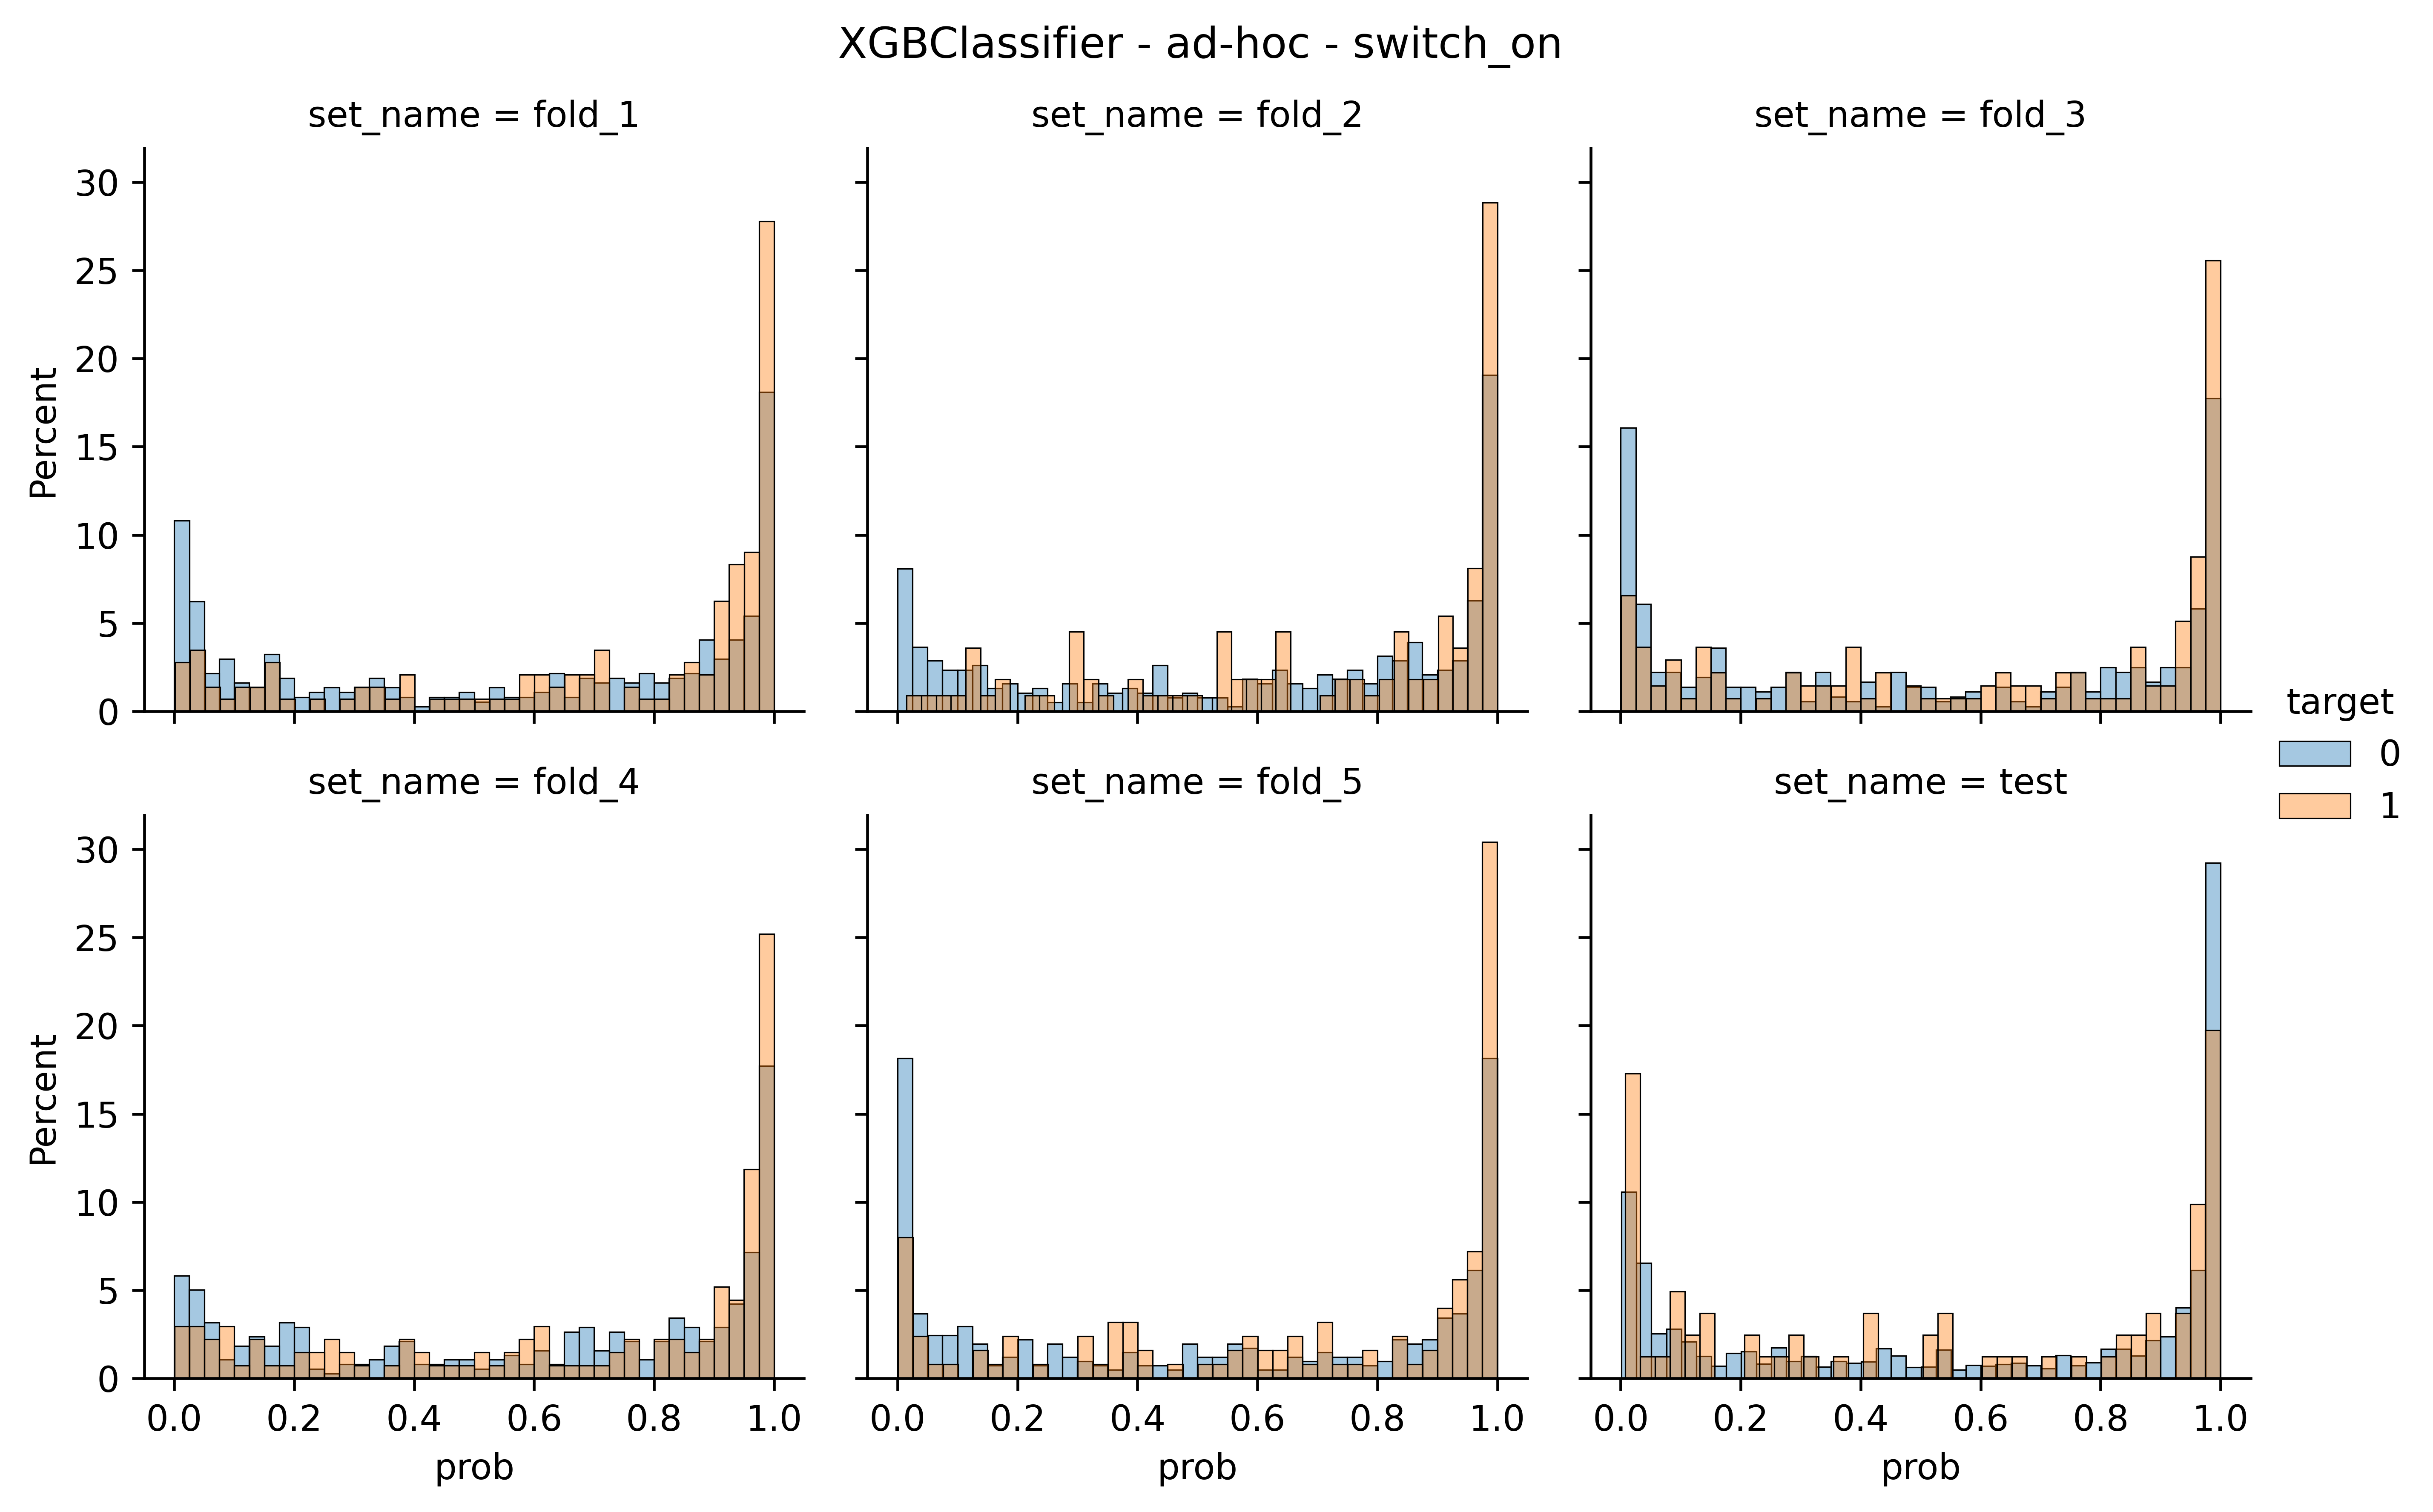
\includegraphics[width=\linewidth]{figures/results/ad-hoc/xgb/switch_on/2021-12-07_06.56.08.418411__distplot.png}
    \end{subfigure}
    \hfill
    \centering
    \begin{subfigure}[b]{0.83\textwidth}
        \centering
        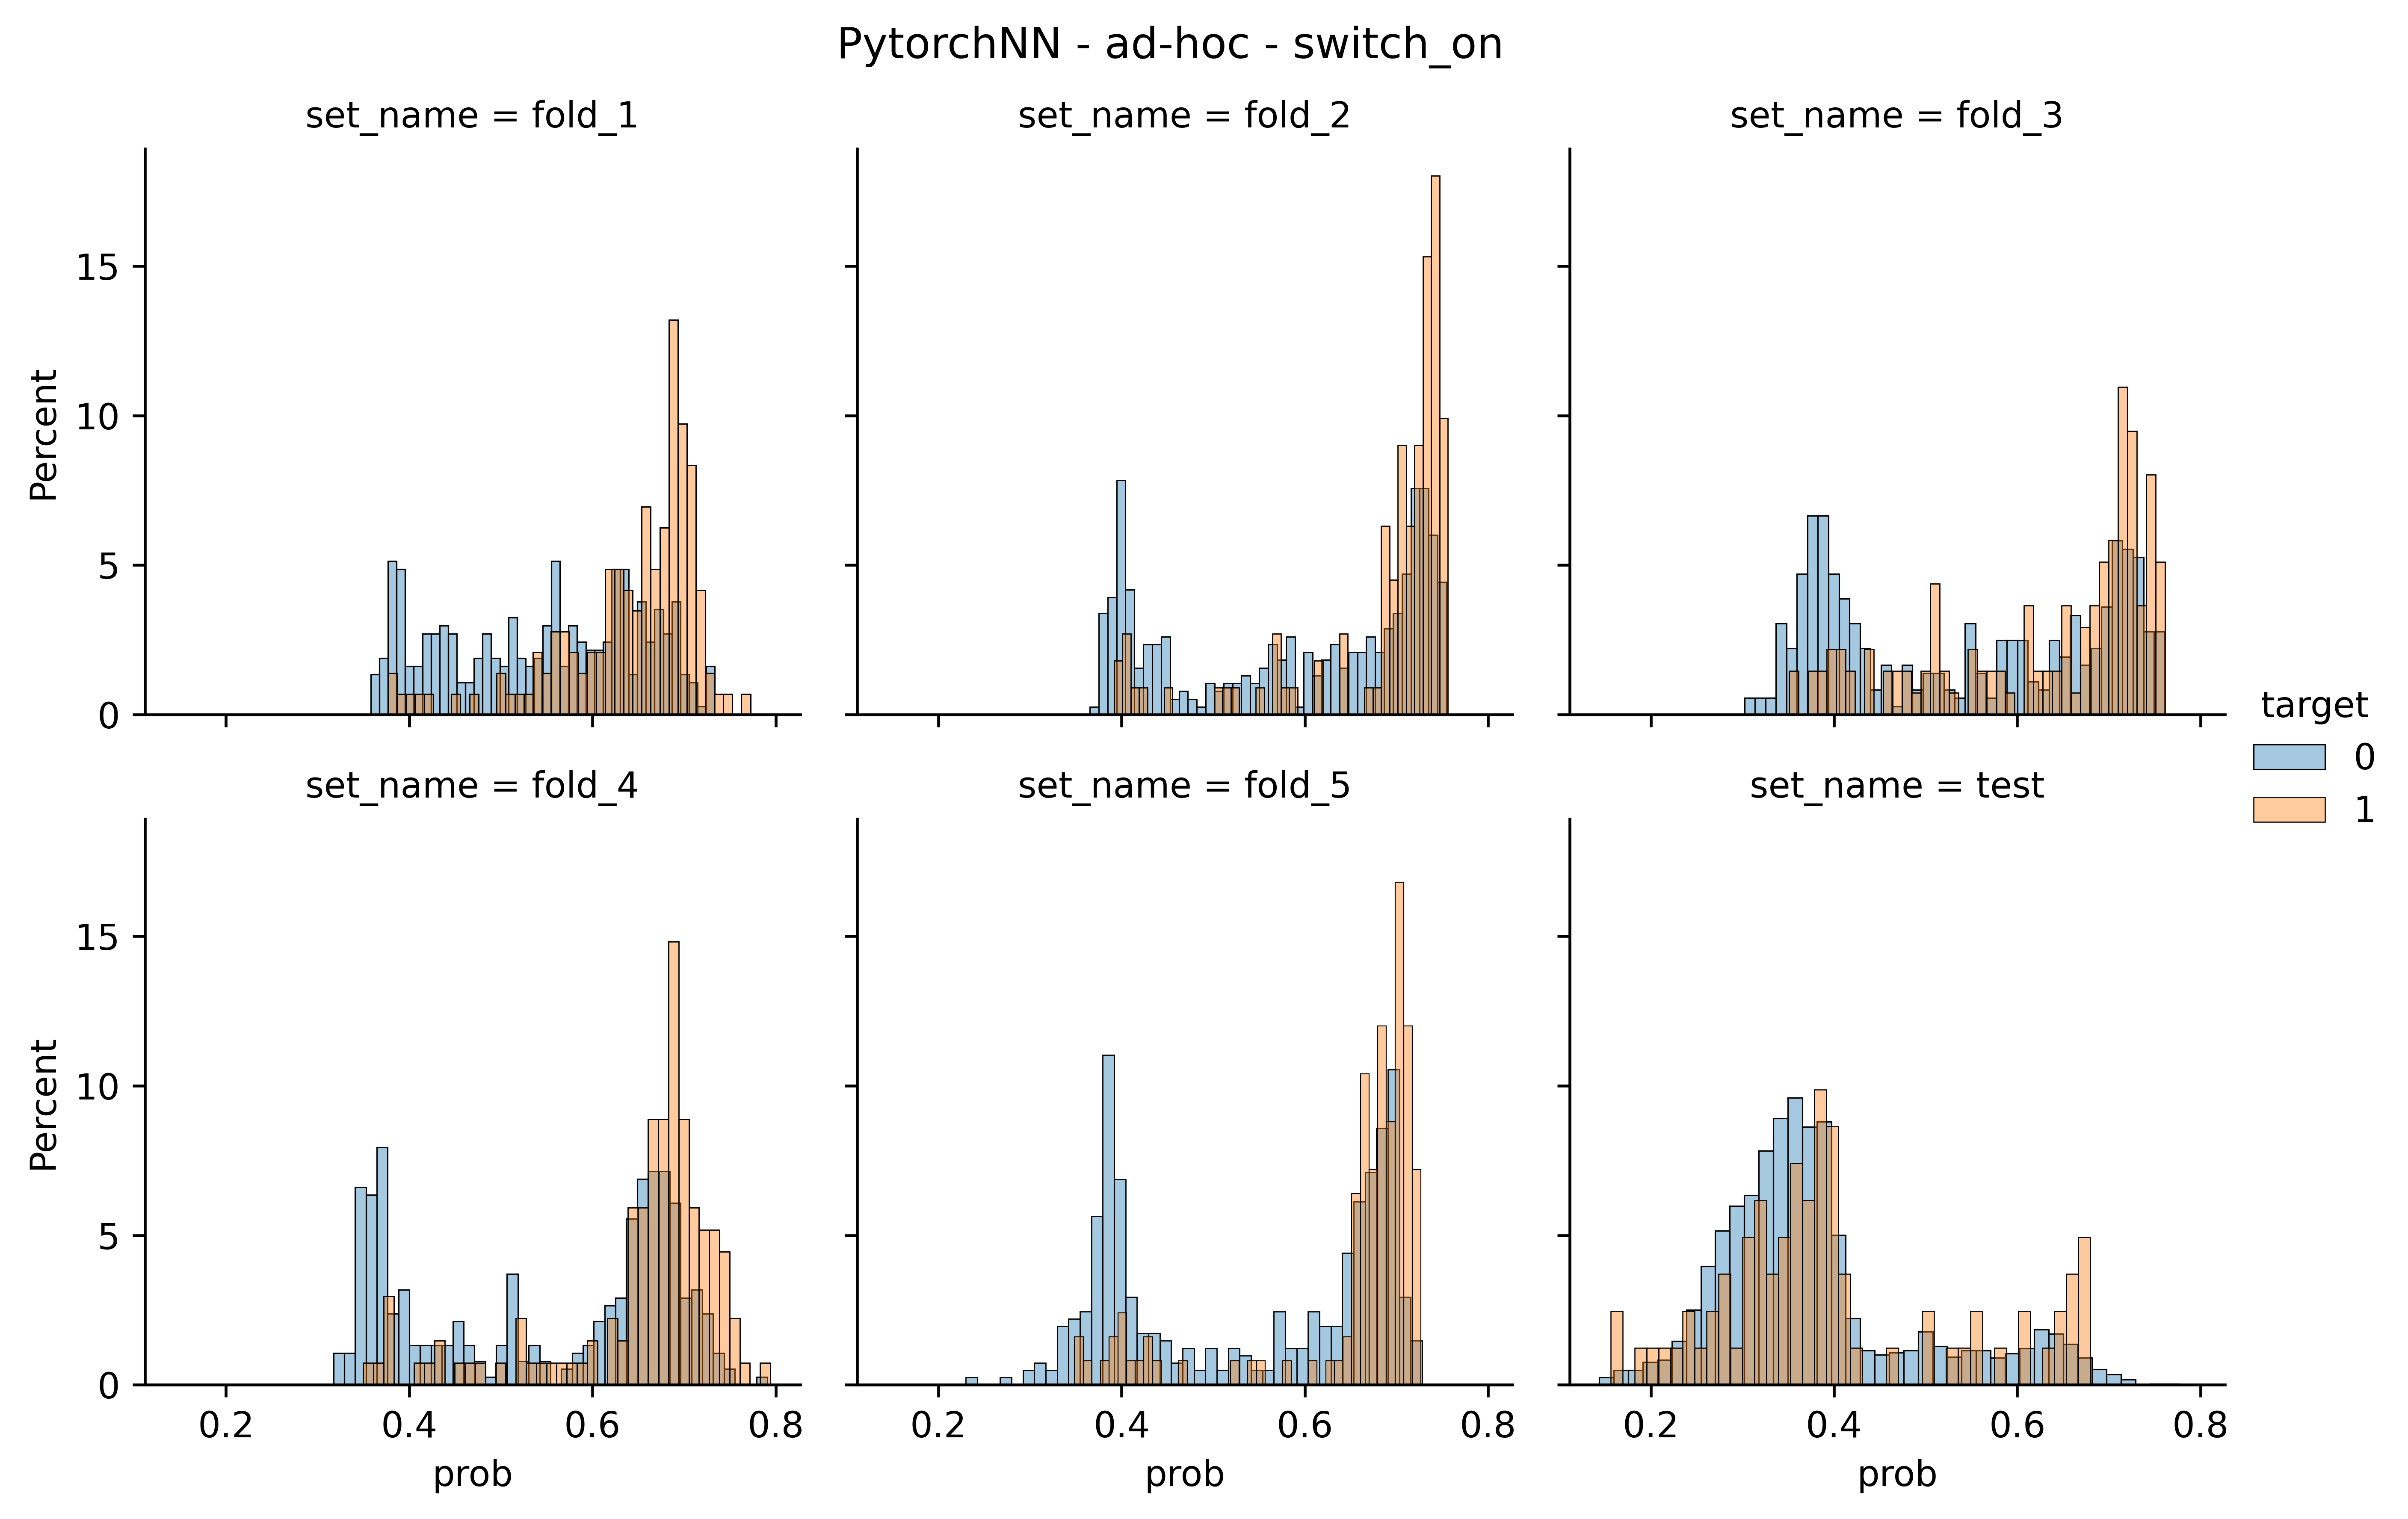
\includegraphics[width=\linewidth]{figures/results/ad-hoc/nn/switch_on/2021-12-06_18.44.35.478500__distplot.png}
    \end{subfigure}
    \caption{Ad-hoc switch\_on}
\end{figure}

\begin{figure}
    \centering
    \begin{subfigure}[b]{0.83\textwidth}
    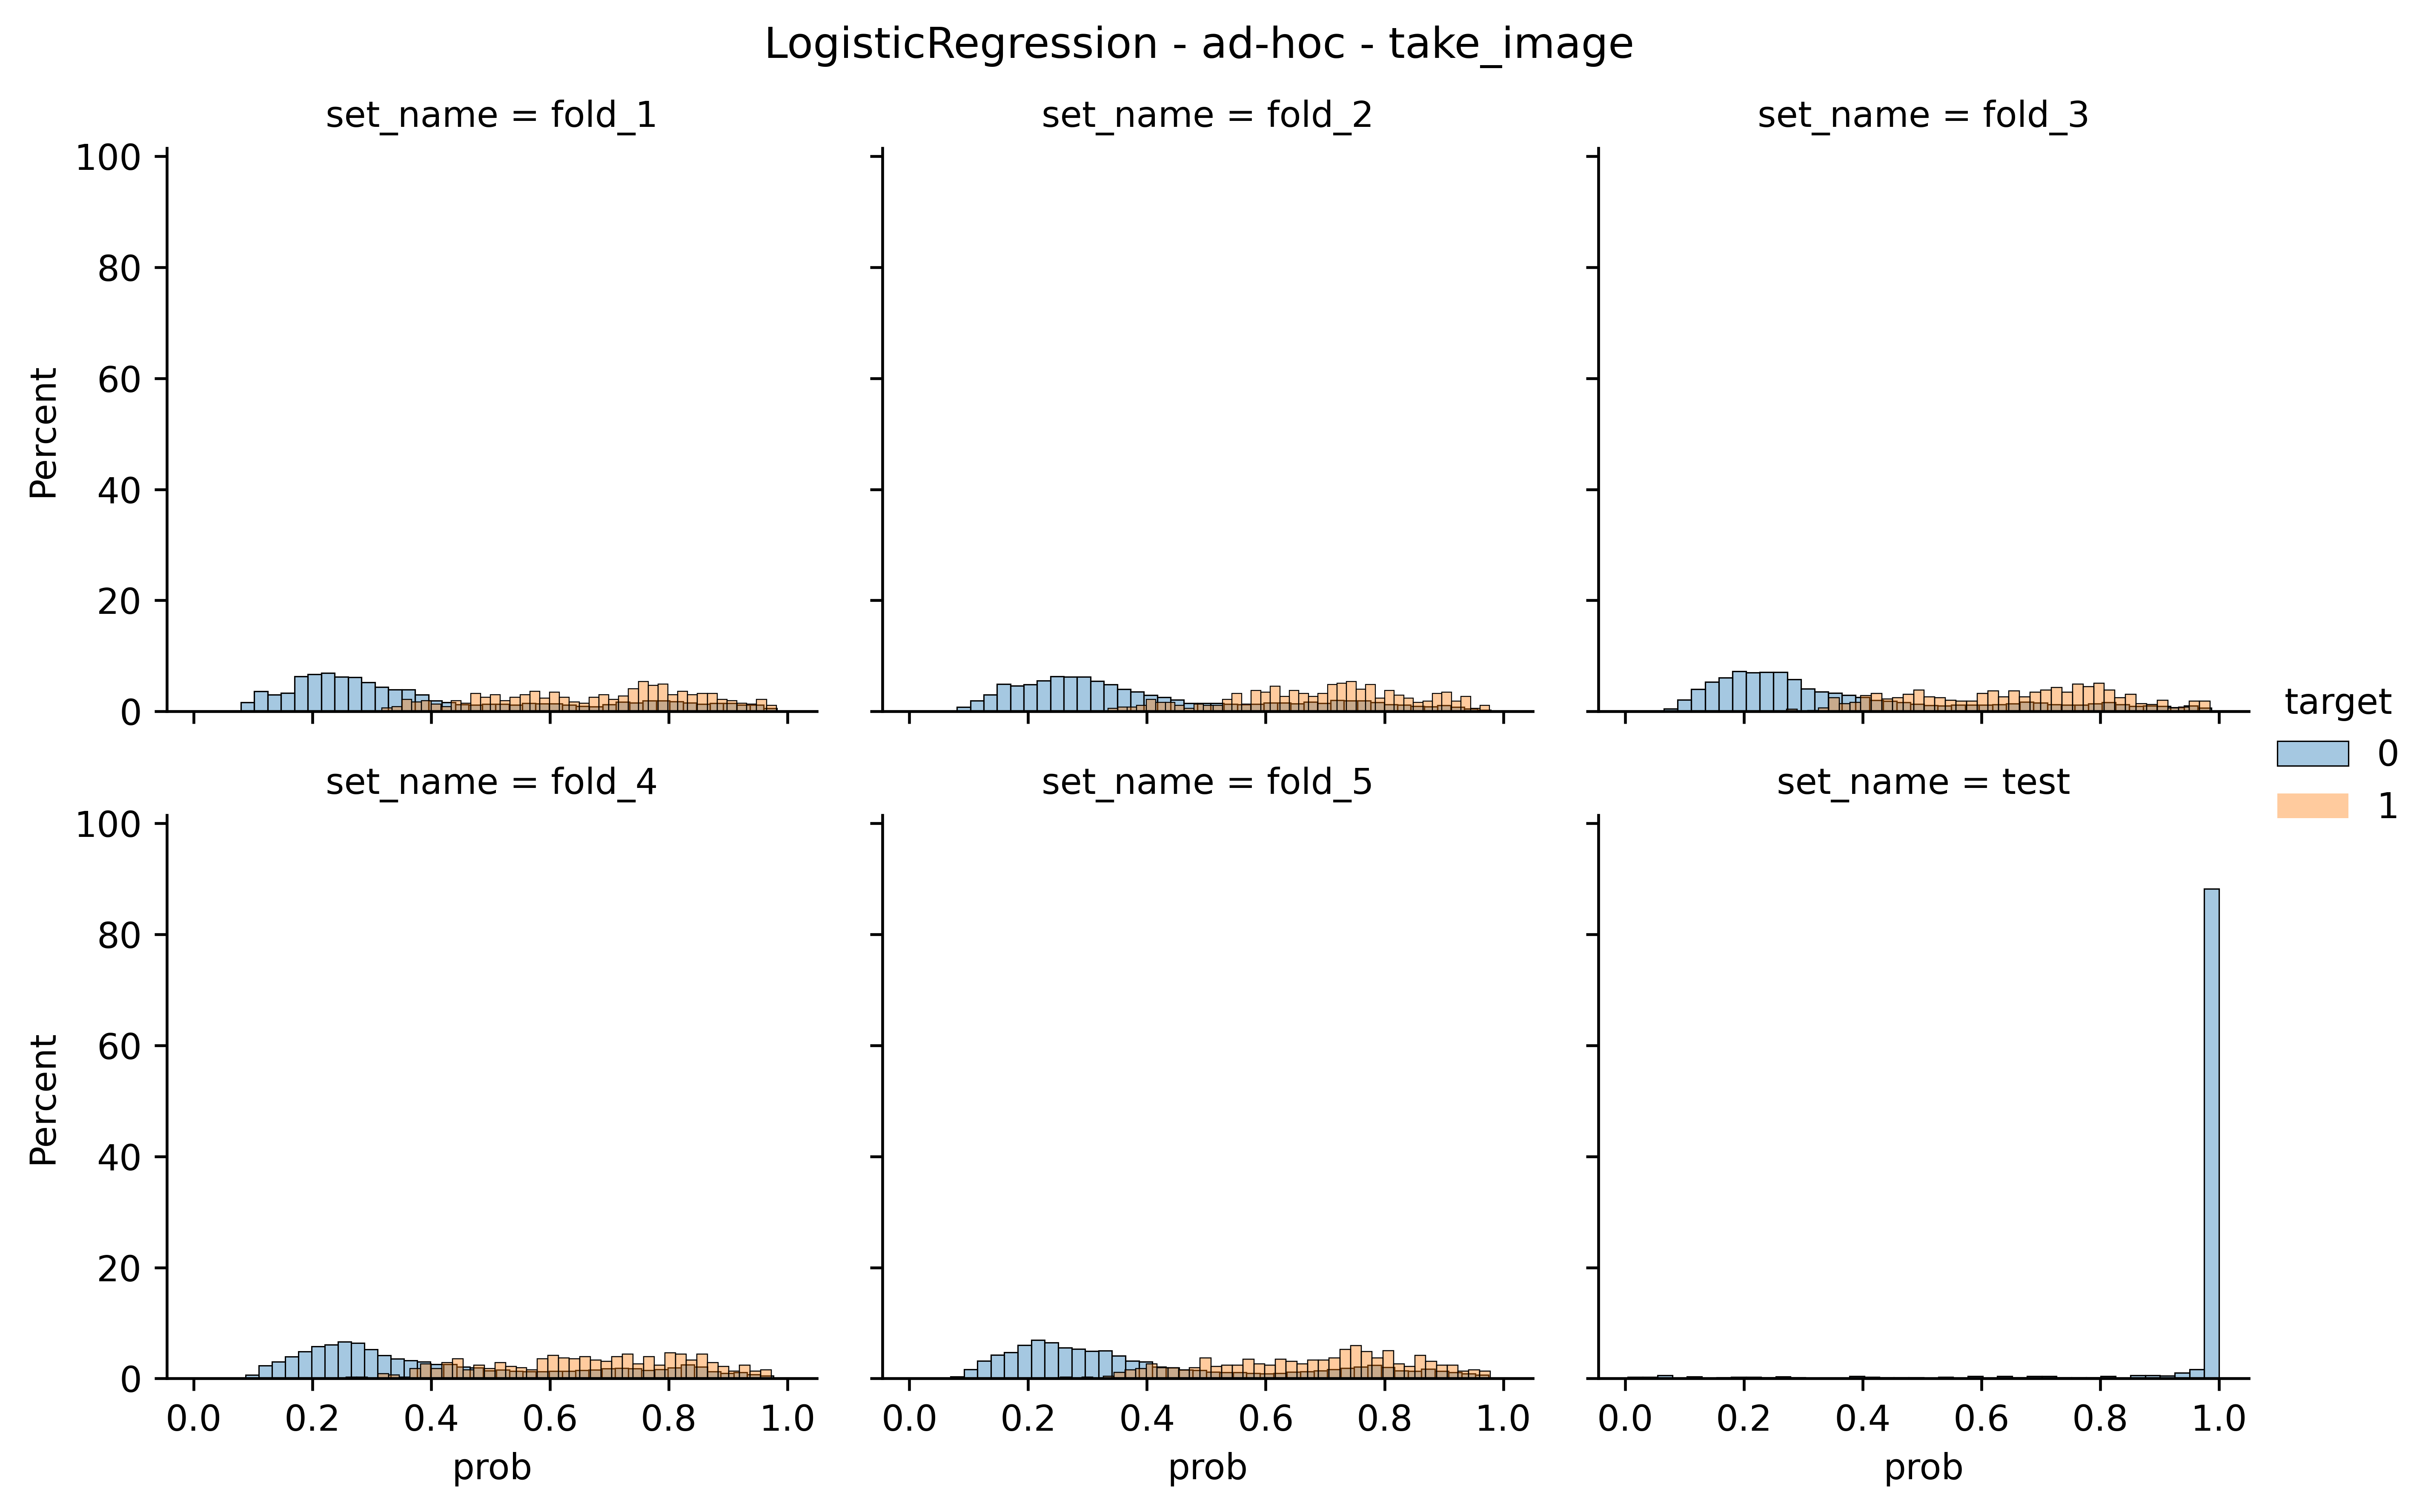
\includegraphics[width=\linewidth]{figures/results/ad-hoc/lgr/take_image/take_image__distplot.png}
    \end{subfigure}
    \hfill
    \centering
    \begin{subfigure}[b]{0.83\textwidth}
        \centering
        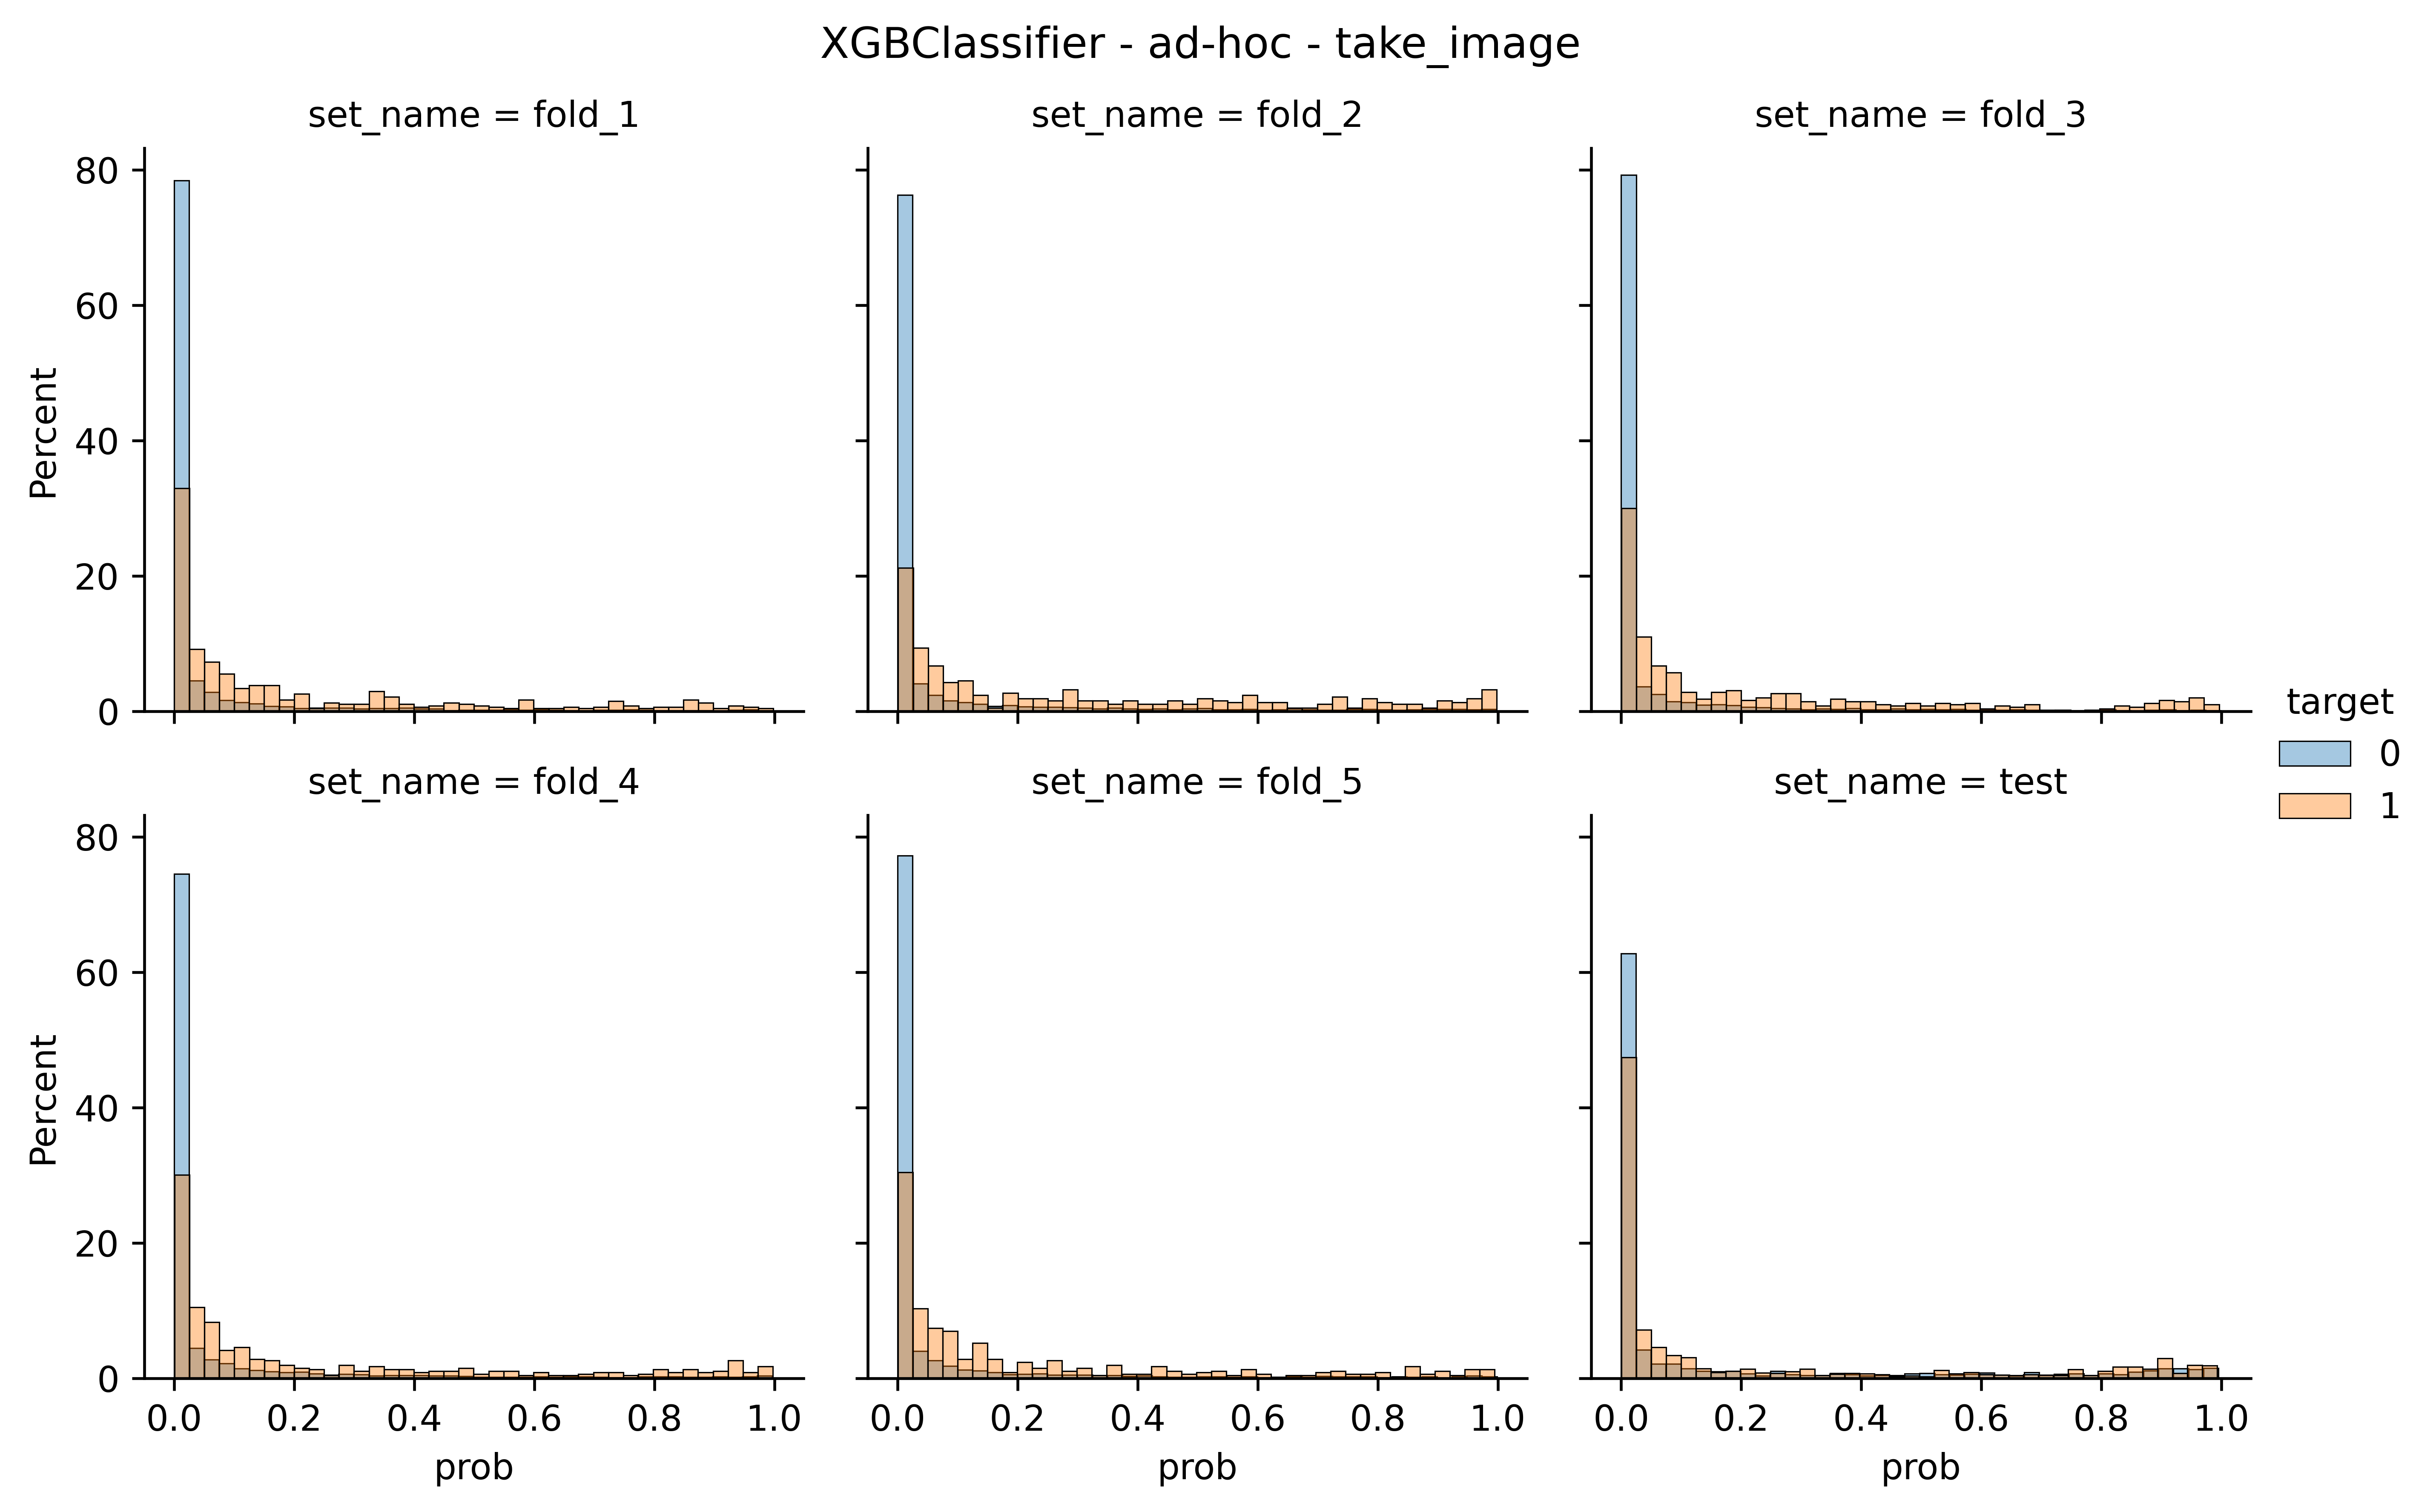
\includegraphics[width=\linewidth]{figures/results/ad-hoc/xgb/2021-12-07_07.38.35.967776__distplot.png}
    \end{subfigure}
    \caption{Ad-hoc take\_image}
\end{figure}

\section{Comparación de mejores modelos}
\label{results:comparison}

\section{Tiempos de predicción}
\label{exp:time}

Para un nuevo ejemplo no visto se debe realizar el proceso completo creación de
ventanas, codificación, predicción por parte del clasificador, y posterior
agrupamiento de ventanas para obtener la máxima prioridad. Al incluir los
modelos predictivos en el proceso de grounding heurístico el tiempo necesario
para realizar todas las etapas y obtener el valor de salida del modelo
predictivo es importante durante el proceso de grounding heurístico ya que los
planificadores deben encontrar la solución a la tarea asignada de acuerdo a un
tiempo límite, si este es excedido, ocurre una falla por parte del planificador.
Esto motivo la medición del tiempo de respuesta para los modelos predictivos
comparados en la sección \ref{results:comparison}.

Actualmente la implementación de grounding heurístico en Fast Downward, son
realizadas a nivel de ejemplo. Por lo que la unidad de medida utilizada fueron
\emph{ns/ejemplo}, no obstante también se probaron realizar las predicciones a
nivel de batch con el de determinar que tan prometedor es incluir este cambio en
el algoritmo de grounding heurístico.

\subsection{Predicciones por batch}

\subsection{Predicciones por acción}

\section{Otros experimentos}

Los experimentos presentados en las secciones \ref{exp:ad-hoc}, \ref{exp:wb}, y
\ref{exp:time} fueron aquellos principales y los que nos enfocamos durante la
tesis. No obstante, se intentaron otras vías de análisis que llevaron a 4
experimentos con el fin de lograr aquel modelo que nos permita guiar el proceso
de grounding. A pesar de no lograr resultados concretos fueron parte importante
del trabajo y otorgaron conocimiento invaluable para involucrarse más en el
dominio del problema.

\subsection{Modelos End-to-end}

End-to-end (E2E) models refieren a sistemas complejos representados por un único
modelo neuronal profundo ensamblando las capas de preprocesamiento y como capas
intermedias del modelo. En particular, este tipo de pruebas se realizaron en una
etapa temprana de la tesis donde la idea de generar ventanas de planes relajados
aún no se había investigado. En particular se experimentaron con modelos E2E de
FastText donde agrega una capa neuronal más al modelo de embeddings para que
sean utilizados en clasificación. No obstante se optó por descontinuar estos
experimentos al comenzar ya que fueron experimentos prototipos donde se buscaba
verificar la factibilidad del uso de word embeddings en grounding heurístico.

\subsection{El problema de inclusión sobre planes relajados}

Otra estrategía que utilizamos durante el análisis en la generación de ventanas
de planes relajados, fue plantear el problema de clasificación binaria como uno
multiclase. En lugar de solo 2 clases, manteníamos 4 que representaban la noción
de si una acción estaba incluido en el plan relajado y si eran parte de los good
operators del problema. Es decir, una ventana de plan relajado $w$ y acción $a$
es etiquetada como:

\begin{itemize}
    \item 0: Si $a$ no es good operator y no pertenece a $w$.
    \item 1: Si $a$ no es good operator y pertenece a $w$.
    \item 2: Si $a$ es good operator y no pertenece a $w$.
    \item 3: Si $a$ es good operator y pertenece a $w$.
\end{itemize}

Luego al agrupar por ventanas y acción, consideramos como predicción final la
clase $3$ si al menos una de las ventanas predijo $3$. Caso contrario si para
alguna ventana la predicción fue $2$ predicción del agrupamiento es $2$. Y así
sucesivamente hasta la clase $0$.

\subsection{Mayorización}

La repetición de ejemplos con etiquetas diferentes puede dificultar el
aprendizaje de un modelo, si no son preprocesadas con alguna técnica de
mayorización. Es decir, de entre todas las repeticiones del mismo ejemplo pero
con distintas clases, mantener una sola replica preservando la etiqueta que haya
ocurrido en mayor cantidad. Esta técnica fue aplicada para la codificación por
word embeddings, donde una hipótesis para mejorar la separación de los ejemplos
de entrenamiento fue asignar la etiqueta mayoritaria para todo los vector de
dimensión $D$ (plan relajado, acción) que estén cerca en un rango en
$\mathbb{R}^{D}$.

\subsection{Orden de ventanas como características}

Por último otra implementación que se agregó al sistema y que es un patrón
configurable de las etapas de ejecución es la posibilidad de mantener el orden
en que ocurren las ventanas. Es decir, se tiene

\begin{table}[h!]
\centering
\scalebox{0.9}{
 \begin{tabular}{||c | c | c | c||} 
 \hline
 Plan relajado & Orden de ventana & Acción & Etiqueta \\ [0.5ex] \hline\hline
 %(take_image satellite0 planet5 instrument1 image1)
 {}[] & 1 &{}[] & 1 \\
 {}[] & 2 &{}[] & 1 \\
 {}[] & 3 &{}[] & 1  \\
 ... & ... & ... & ...\\ [1ex] 
 \hline
 \end{tabular}}
 \caption{Ejemplos etiquetados a partir de un plan relajado y una acción}
 \label{tb:matrix_shape}
\end{table}

El objetivo de este agregado es evitar perder la información del orden durante
la separación y se buscaba analizar si es un factor relevante para el
entrenamiento y evaluación.
    \chapter{Conclusions and Future Work}
\label{ch:con}
\section{Conclusions}
Typically a conclusions chapter first summarizes the investigated problem and its aims and objectives. It summaries the critical/significant/major findings/results about the aims and objectives that have been obtained by applying the key methods/implementations/experiment set-ups. A conclusions chapter draws a picture/outline of your project's central and the most signification contributions and achievements. 

A good conclusions summary could be approximately 300--500 words long, but this is just a recommendation.

A conclusions chapter followed by an abstract is the last things you write in your project report.

\section{Future work}
This section should refer to Chapter~\ref{ch:results} where the author has reflected their criticality about their own solution. The future work is then sensibly proposed in this section.

\textbf{Guidance on writing future work:} While working on a project, you gain experience and learn the potential of your project and its future works. Discuss the future work of the project in technical terms. This has to be based on what has not been yet achieved in comparison to what you had initially planned and what you have learned from the project. Describe to a reader what future work(s) can be started from the things you have completed. This includes identifying what has not been achieved and what could be achieved. 



A good future work summary could be approximately 300--500 words long, but this is just a recommendation.
    \chapter{Reflection}
\label{ch:reflection}
%%%%%%%%%%%%%%%%%%%%%%%%%%%%%%%
%% Please remove/replace text below
%%%%%%%%%%%%%%%%%%%%%%%%%%%%%%%
Write a short paragraph on the substantial learning experience. This can include your decision-making approach in problem-solving.

\textbf{Some hints:} You obviously learned how to use different programming languages, write reports in \LaTeX and use other technical tools. In this section, we are more interested in what you thought about the experience. Take some time to think and reflect on your individual project as an experience, rather than just a list of technical skills and knowledge. You may describe things you have learned from the research approach and strategy, the process of identifying and solving a problem, the process research inquiry, and the understanding of the impact of the project on your learning experience and future work.

Also think in terms of:
\begin{itemize}
    \item what knowledge and skills you have developed
    \item what challenges you faced, but was not able to overcome
    \item what you could do this project differently if the same or similar problem would come
    \item rationalize the divisions from your initial planed aims and objectives.
\end{itemize}


A good reflective summary could be approximately 300--500 words long, but this is just a recommendation.

~\\[2em]
\noindent
{\huge \textbf{Note:}} The next chapter is ``\textbf{References},'' which will be automatically generated if you are using BibTeX referencing method. This template uses BibTeX referencing.  Also, note that there is difference between ``References'' and ``Bibliography.'' The list of ``References'' strictly only contain the list of articles, paper, and content you have cited (i.e., refereed) in the report. Whereas Bibliography is a list that contains the list of articles, paper, and content you have cited in the report plus the list of articles, paper, and content you have read in order to gain knowledge from. We recommend to use only the list of ``References.'' 

    
    % -------------------------------------------------------------------
    % Bibliography/References
    % -------------------------------------------------------------------
    \bibliographystyle{agsm}
    
    \bibliography{references}
    
    % -------------------------------------------------------------------
    % Appendices
    % -------------------------------------------------------------------
    
    \begin{appendices}
        \chapter{An Appendix Chapter (Optional)}
\label{appn:A}
    \end{appendices}
    
\end{document}
